%%%%%%%% ICML 2026 — EvTOL-Traj Research Paper %%%%%%%%%%%%%%%%%%%%%%%%%%%

\documentclass{article}

\usepackage{microtype}
\usepackage{graphicx}
\usepackage{subcaption}
\usepackage{booktabs}
\usepackage{hyperref}
\newcommand{\theHalgorithm}{\arabic{algorithm}}

% Blind review submission
\usepackage{icml2026}

\usepackage{amsmath}
\usepackage{amssymb}
\usepackage{mathtools}
\usepackage{amsthm}
\usepackage{multirow}
\usepackage{array}
\usepackage{xcolor}
\usepackage[capitalize,noabbrev]{cleveref}

\theoremstyle{plain}
\newtheorem{theorem}{Theorem}[section]
\newtheorem{proposition}[theorem]{Proposition}
\newtheorem{lemma}[theorem]{Lemma}
\theoremstyle{definition}
\newtheorem{definition}[theorem]{Definition}
\newtheorem{assumption}[theorem]{Assumption}

\icmltitlerunning{Physics-Grounded Multi-Task Learning for Defense eVTOL Missions}

\begin{document}

\twocolumn[
  \icmltitle{Physics-Grounded Multi-Task Learning for\\
    Defense Electric Vertical Takeoff and Landing Mission Prediction}

  \icmlsetsymbol{equal}{*}

  \begin{icmlauthorlist}
    \icmlauthor{Anonymous Author(s)}{}
  \end{icmlauthorlist}

  \icmlkeywords{Multi-task learning, autonomous systems, defense AI,
    trajectory optimization, eVTOL, class imbalance, physics simulation}

  \vskip 0.3in
]

\printAffiliationsAndNotice{}

% =====================================================================
\begin{abstract}
% =====================================================================
We study multi-task prediction for defense electric vertical takeoff and
landing (eVTOL) autonomous missions, where a four-layer causal simulation
stack---perception, trajectory planning, vehicle dynamics, and flight
control---produces 373 physics-grounded features per mission record.
We introduce \textbf{EvTOL-Traj}, a dataset of 400{,}000 complete mission
records across sixteen geographically diverse Indian regions spanning
urban airspace, high-altitude desert, mountain border terrain, and maritime
theatres, each annotated with real SRTM terrain, Open-Meteo wind forecasts,
OpenStreetMap obstacle inventories, and analytical surface-to-air missile
(SAM) threat models.
We formalize four machine learning tasks on this dataset and present
a pure-NumPy single-task neural network baseline that achieves
AUC-ROC $\geq 0.97$ on threat risk classification and $R^2 \geq 0.77$
on energy consumption regression across six regions with sufficient class support.
Critically, we characterize three systematic challenges that limit
out-of-the-box multi-task learners on this data: severe geographically
induced class imbalance (positive rates spanning 0.1\%--96.6\%), distribution
shift across terrain regimes, and cross-layer feature leakage arising from
the causal simulation structure.
These findings position EvTOL-Traj as a demanding benchmark for
safety-critical multi-task learning under geographic distribution shift.
\end{abstract}

% =====================================================================
\section{Introduction}
\label{sec:intro}
% =====================================================================

The electric vertical takeoff and landing (eVTOL) platform has emerged as a
dual-use technology combining rotor hover flexibility with fixed-wing cruise
efficiency \citep{garrow2021urban,johnson2020nasa}.
In defense contexts, eVTOLs are envisioned for logistics resupply under fire,
reconnaissance in denied-access areas, and autonomous swarm coordination---missions
requiring safe navigation through active surface-to-air missile (SAM) threat
environments \citep{dod2022autonomy}.

\textbf{The machine learning challenge.}
A defense eVTOL autonomous mission involves a \emph{causally linked} four-layer
pipeline:
(1) a \emph{perception} layer that fuses terrain, wind, obstacle, and SAM threat
fields into a cost map;
(2) a \emph{planning} layer that uses RRT* \citep{karaman2011sampling} and
NSGA-III \citep{deb2014evolutionary} to find Pareto-optimal threat-avoiding
trajectories;
(3) a \emph{vehicle dynamics} layer that simulates blade element momentum,
battery electrochemistry, motor thermodynamics, acoustic, infrared, and
radar signatures; and
(4) a \emph{flight control} layer that evaluates 50\,Hz cascaded PID tracking fidelity.
Each layer conditions on the previous one, creating a structured causal graph
that is simultaneously a source of rich multi-output supervision and a minefield
for data leakage in cross-layer evaluation.

\textbf{Gap in existing work.}
Existing ML benchmarks for autonomous air vehicles address individual layers
in isolation---UAV path planning \citep{ong2021uav},
energy modeling \citep{rodrigues2021energy,nakamura2023energy},
or radar threat analysis \citep{bodner1994radar,skolnik2008radar}---but none
provides a multi-layer causally linked dataset suited for studying multi-task
prediction of mission outcomes.
General multi-task learning \citep{caruana1997multitask,ruder2017overview}
benefits greatly from datasets with heterogeneous, correlated outputs generated by
a shared underlying process; eVTOL simulation provides exactly this structure.

\textbf{Our contributions:}
\begin{enumerate}
  \item \textbf{EvTOL-Traj dataset}: 400{,}000 complete mission records
    across 16 Indian geographic regions with 373 physics-grounded features.
    The dataset is generated by a fully open-source pipeline connecting
    real geospatial data sources (SRTM, Open-Meteo, OpenStreetMap) with
    high-fidelity physical simulation.
  \item \textbf{Four benchmark tasks} (T1--T4) on threat risk classification,
    energy regression, threat regression, and control tracking error prediction,
    with a strict cross-layer leak-free evaluation protocol.
  \item \textbf{Systematic characterization} of three failure modes for
    standard multi-task learners on this data: geographic class imbalance,
    cross-region distribution shift, and causal feature leakage.
  \item \textbf{Single-task neural network baseline} (pure NumPy, no ML
    framework dependency) with detailed ablation by region, task, and
    class weight scheme.
\end{enumerate}

% =====================================================================
\section{Related Work}
\label{sec:related}
% =====================================================================

\paragraph{Multi-task learning.}
Shared-representation MTL \citep{caruana1997multitask} improves sample
efficiency and regularization when tasks share underlying structure.
\citet{ruder2017overview} surveys hard and soft parameter sharing;
\citet{liu2019end} demonstrates attention-gated task routing.
Key open problems include task weighting under imbalanced losses
\citep{wu2020understanding} and cross-task interference---both
prominent in our benchmark.

\paragraph{Safety-critical and physics-grounded ML.}
Recent work integrates physical constraints into neural architectures for
aerospace \citep{reiss2024safety}.
Our dataset differs in providing \emph{complete simulation-layer supervision}
rather than physics-informed priors, enabling data-driven study of
the full mission stack without analytical surrogate assumptions.

\paragraph{Distribution shift in autonomous systems.}
Geographic distribution shift is a known challenge for autonomous
vehicle models \citep{ben2010theory,sagawa2020distributionally}.
EvTOL-Traj introduces a controlled geographic shift benchmark: sixteen
regions span $> 3{,}000$\,km and three distinct climate/terrain regimes,
making explicit region-level train/test splits a natural experimental design.

\paragraph{Class imbalance.}
SAM threat geography creates extreme and predictable label imbalance
(Section~\ref{sec:analysis}), ranging from 0.1\% to 96.6\% positive rate.
Standard reweighting \citep{he2009learning} partially mitigates this;
we characterize residual failure modes.

% =====================================================================
\section{Dataset}
\label{sec:dataset}
% =====================================================================

\subsection{Simulation Pipeline}

EvTOL-Traj is generated by a four-layer open-source simulation pipeline.
Figure~\ref{fig:pipeline} illustrates the causal structure.
Each layer conditions fully on its predecessors, and all random seeds are
region-specific and fixed for reproducibility.

\begin{figure*}[t]
  \vskip 0.2in
  \begin{center}
    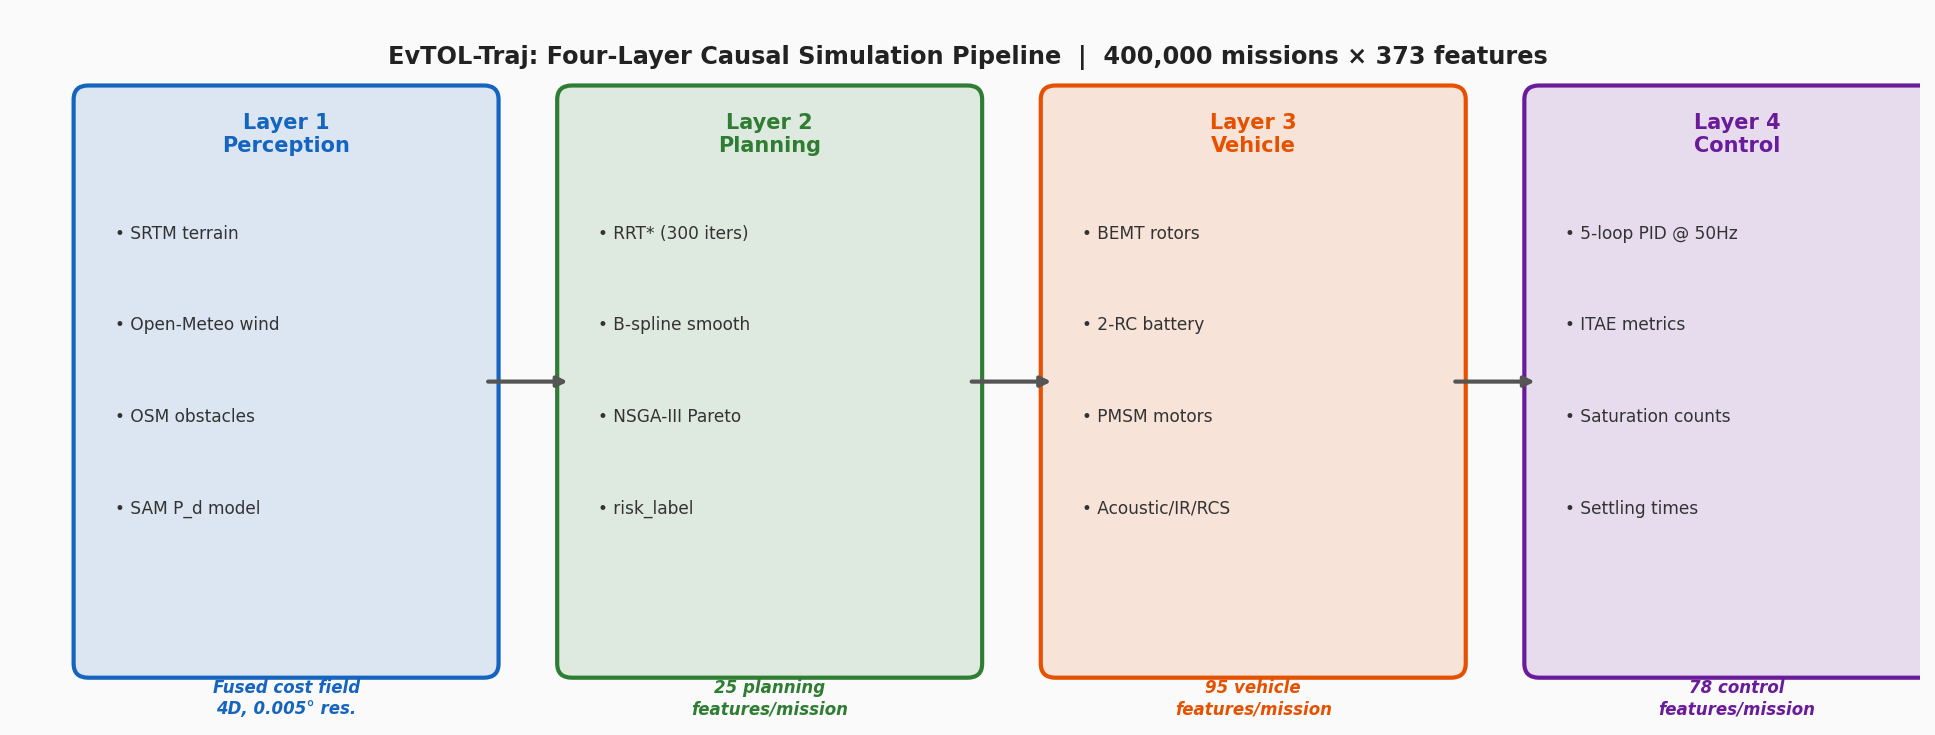
\includegraphics[width=\textwidth]{fig_pipeline.png}
    \caption{EvTOL-Traj four-layer causal simulation pipeline. Each layer
      conditions on all prior layers. The dataset records 373 physics-grounded
      features per mission across the four layers.}
    \label{fig:pipeline}
  \end{center}
  \vskip -0.2in
\end{figure*}

\begin{figure}[t]
  \vskip 0.2in
  \begin{center}
    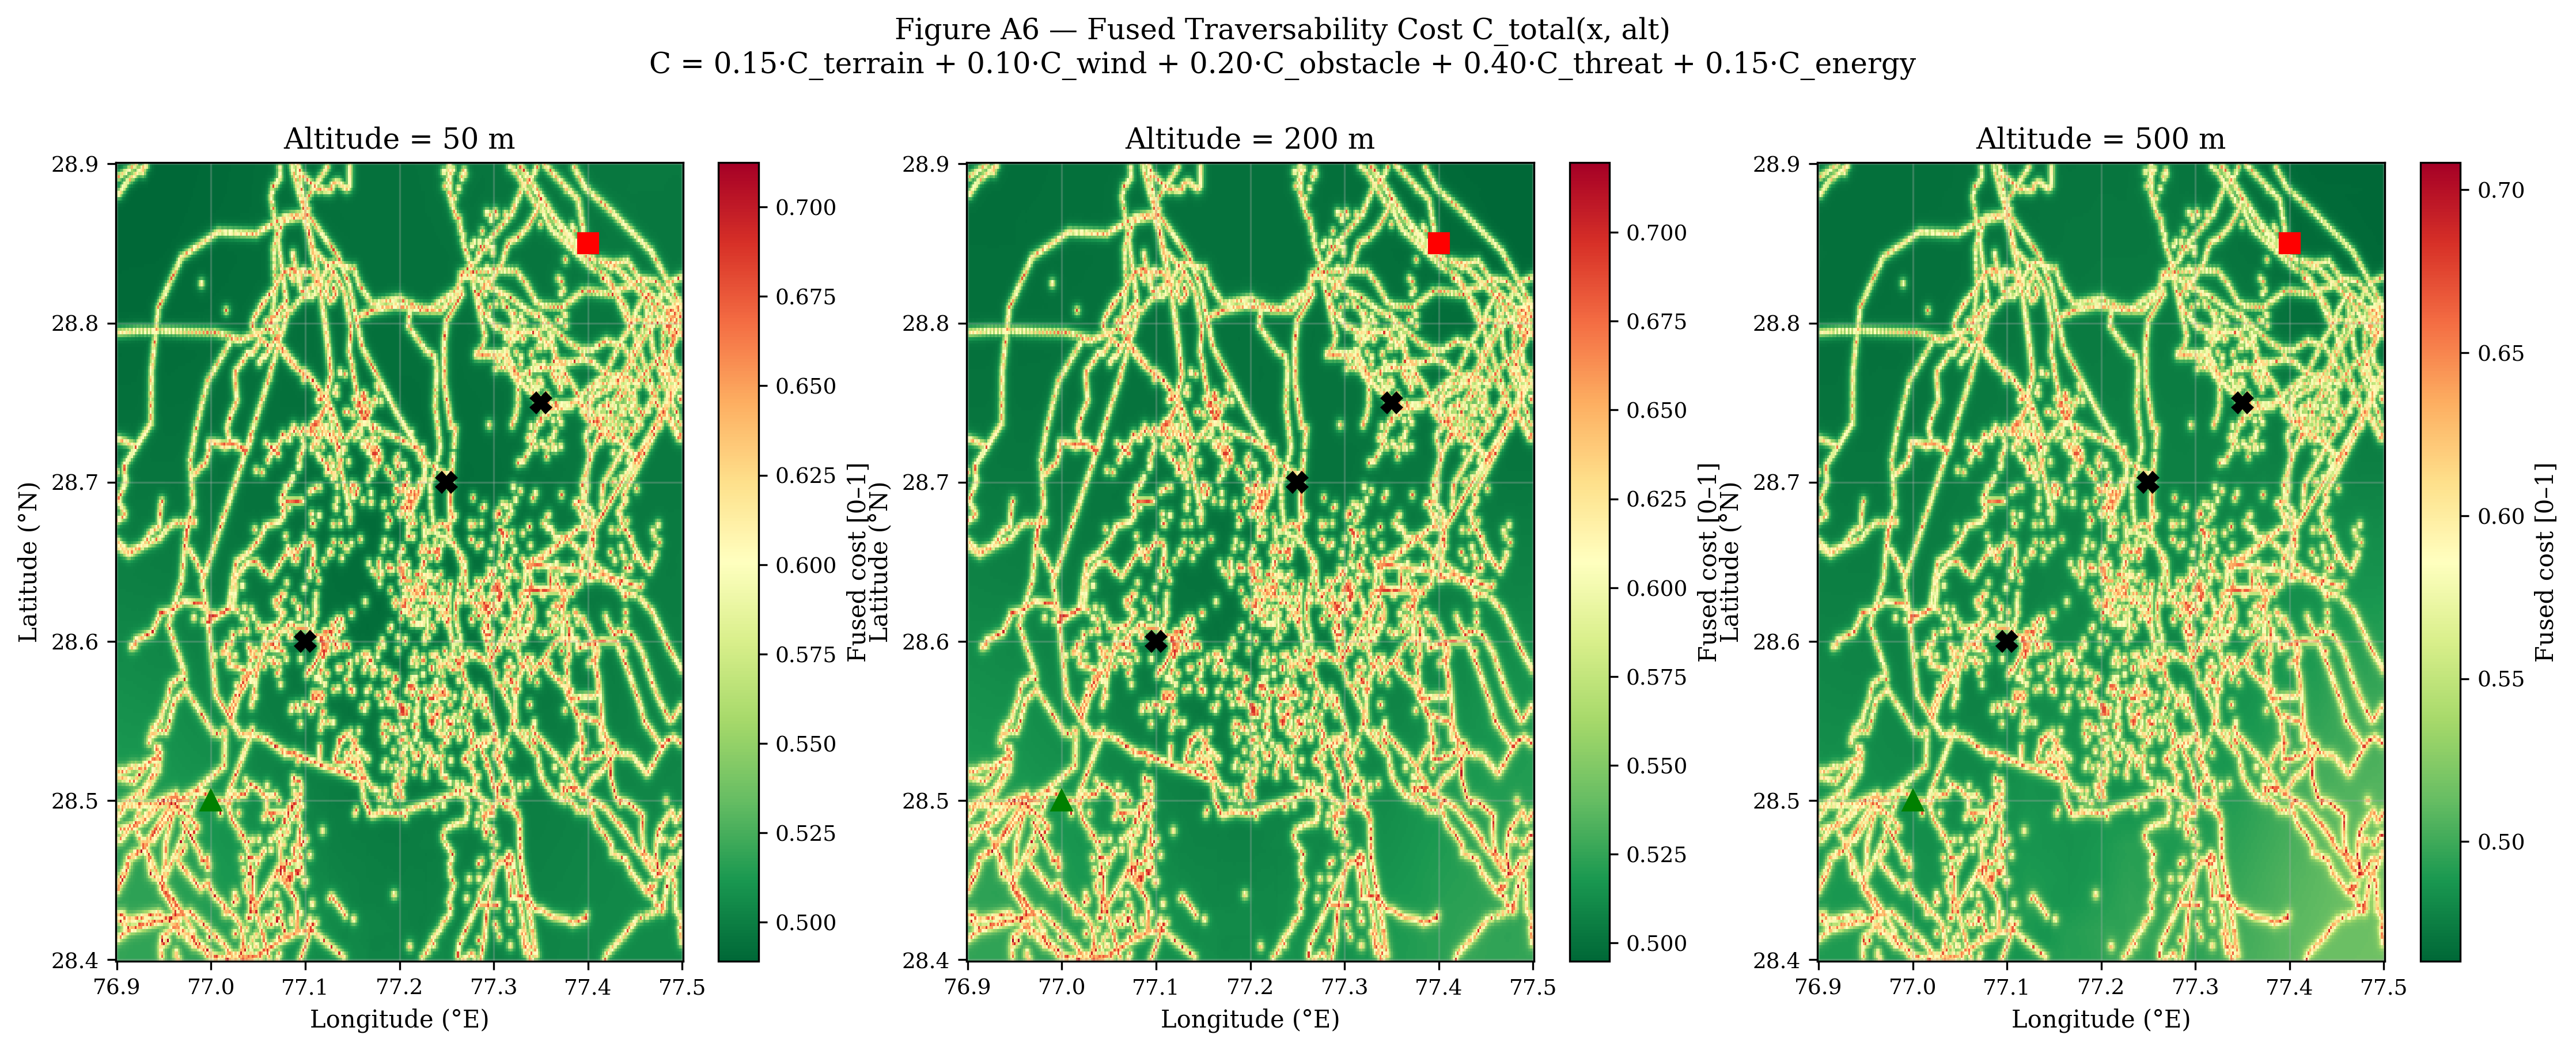
\includegraphics[width=\columnwidth]{figures/perception_A6_fused_cost_map.png}
    \caption{Delhi fused perception cost field: SAM threat probability
      contours overlaid on terrain, wind, and obstacle cost components.
      The 0.35 risk threshold separates high- and low-risk zones.}
    \label{fig:fused_cost}
  \end{center}
  \vskip -0.2in
\end{figure}

\begin{figure*}[t]
  \vskip 0.2in
  \begin{center}
    \begin{subfigure}[b]{0.32\textwidth}
      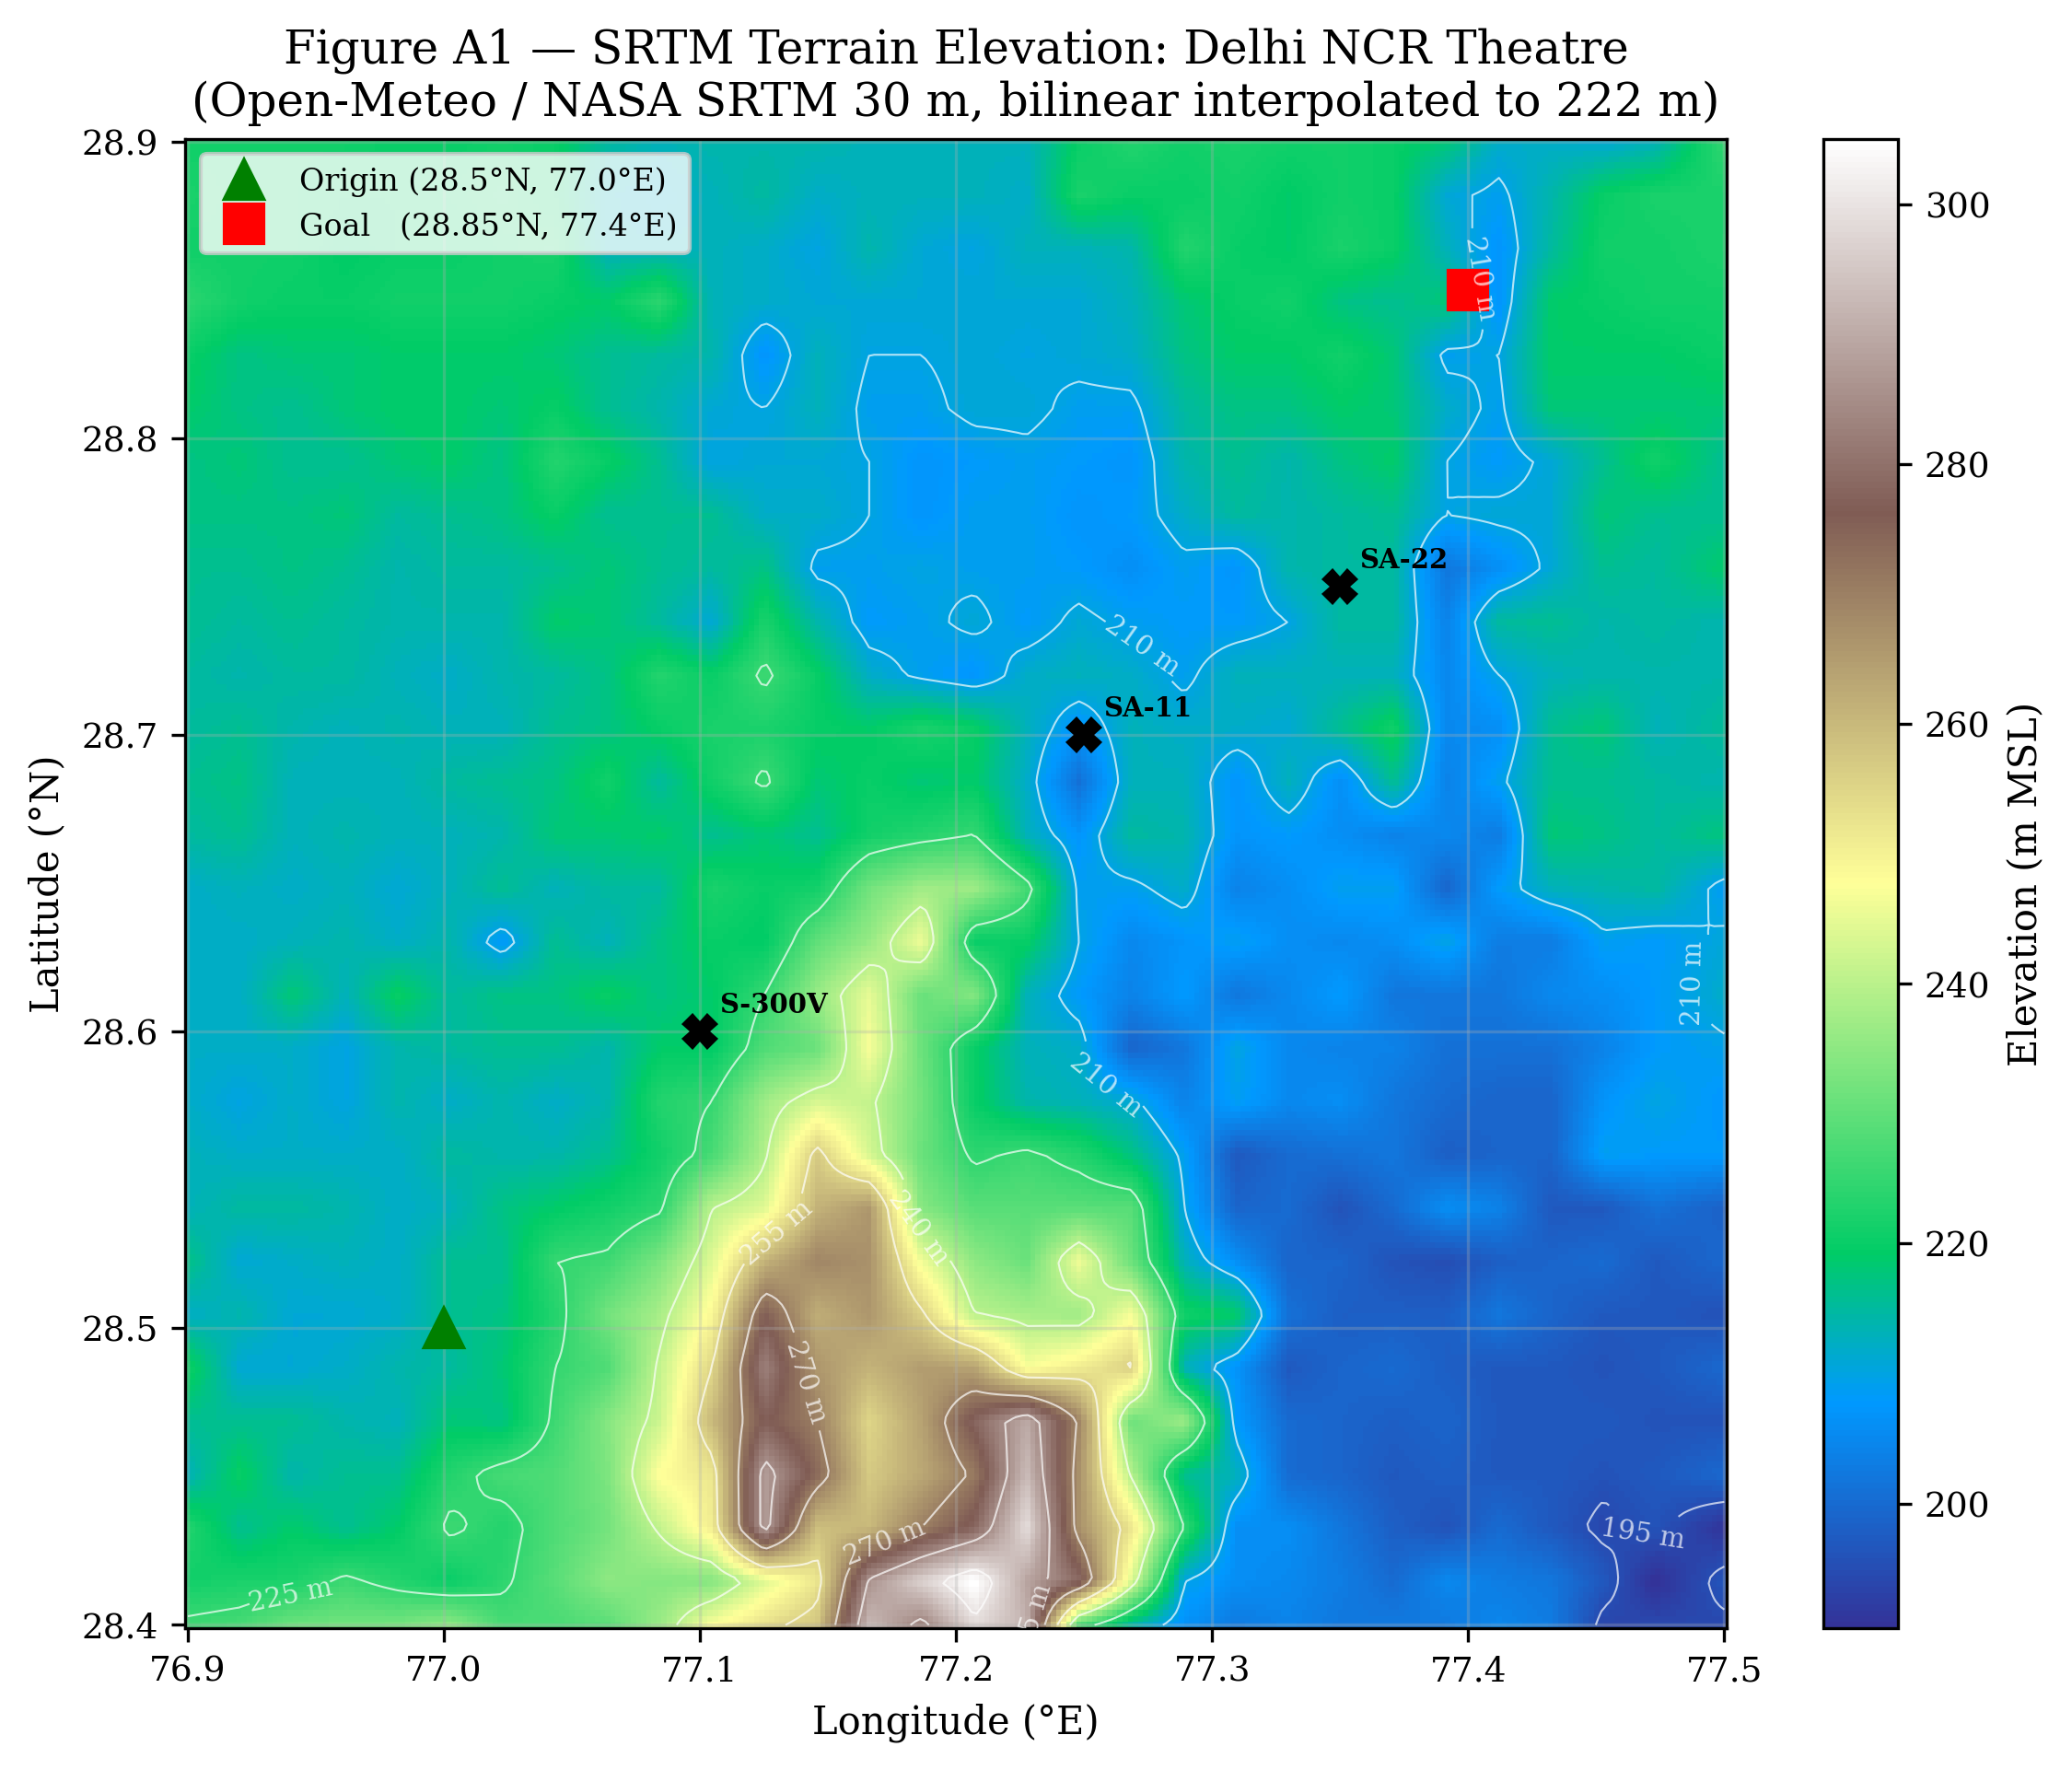
\includegraphics[width=\textwidth]{figures/perception_A1_terrain_elevation.png}
      \caption{Terrain elevation (SRTM)}
    \end{subfigure}
    \hfill
    \begin{subfigure}[b]{0.32\textwidth}
      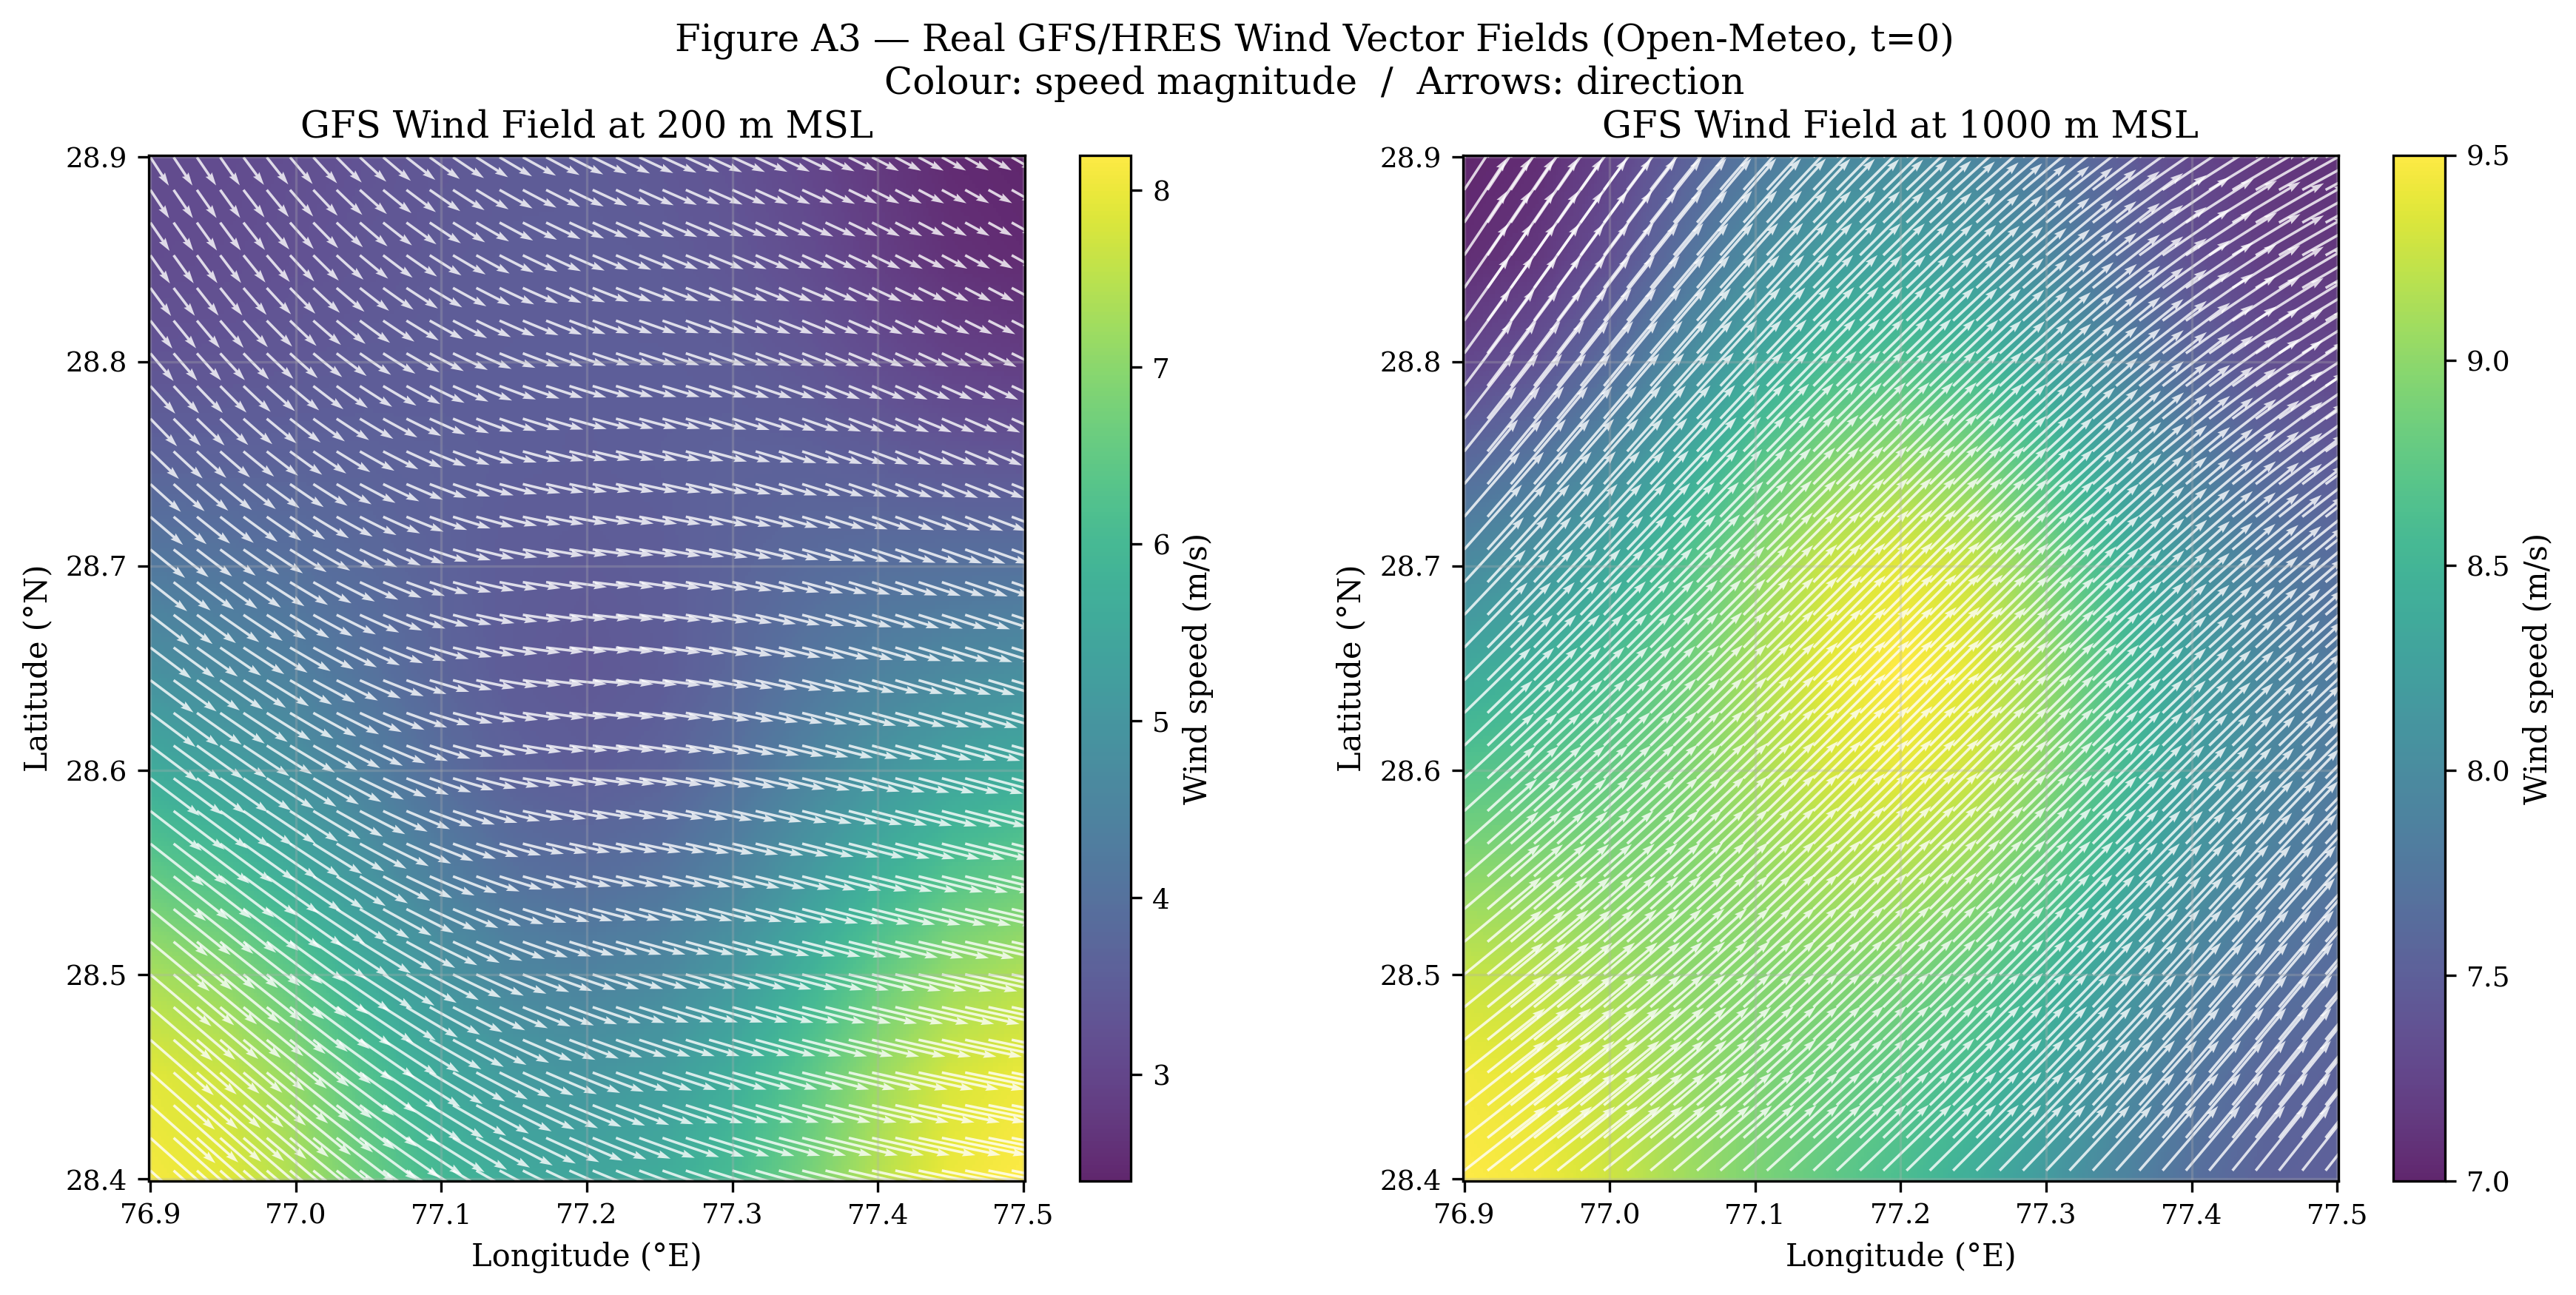
\includegraphics[width=\textwidth]{figures/perception_A3_wind_quiver.png}
      \caption{ERA5 wind field}
    \end{subfigure}
    \hfill
    \begin{subfigure}[b]{0.32\textwidth}
      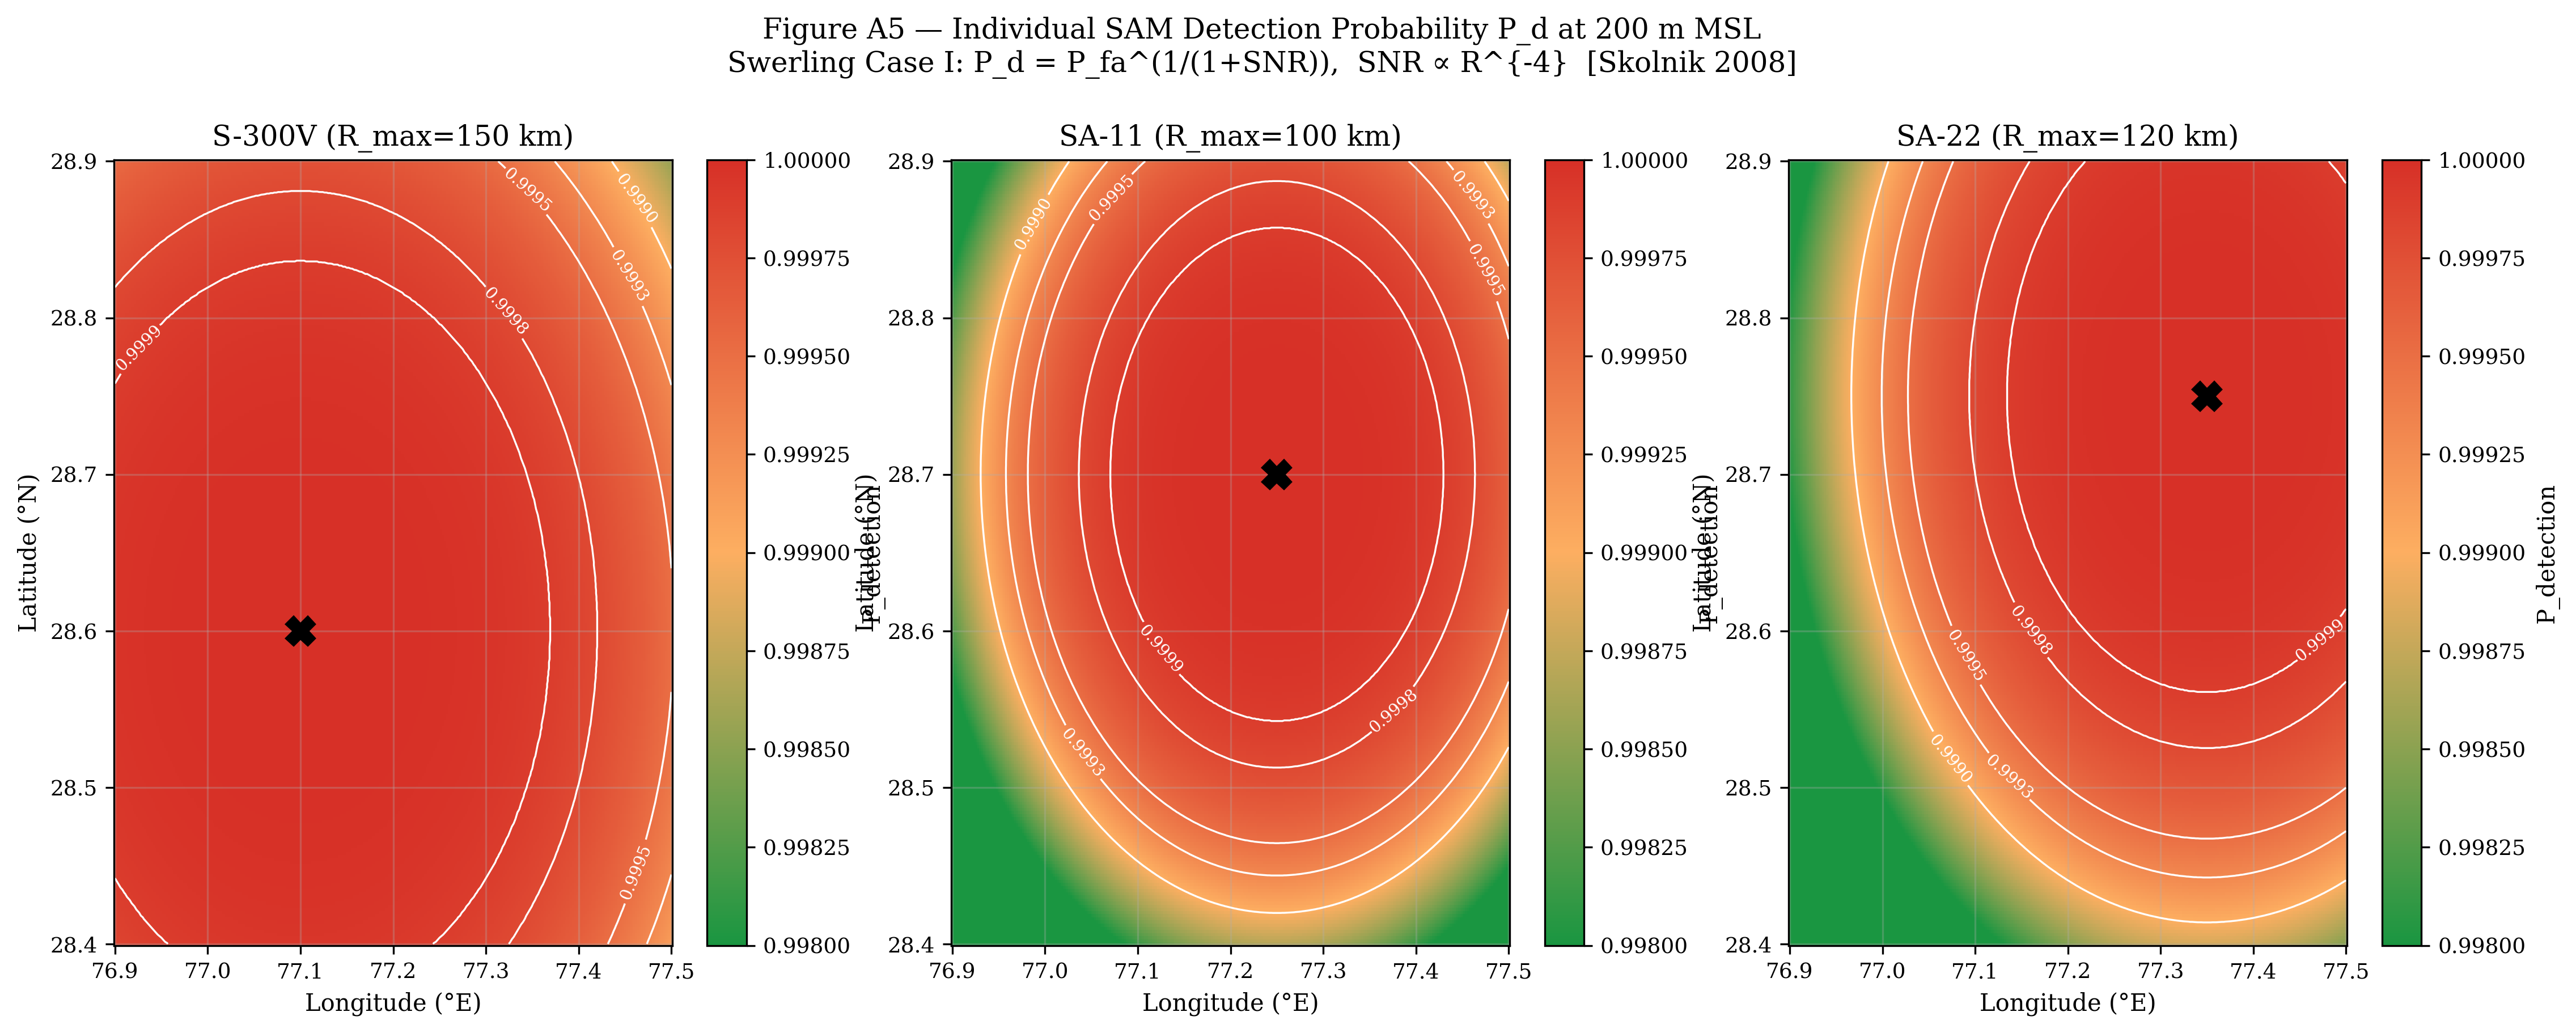
\includegraphics[width=\textwidth]{figures/perception_A5_threat_pd_contours.png}
      \caption{SAM $P_d$ contours}
    \end{subfigure}
    \caption{The three primary perception cost components for Delhi.
      Terrain cost (left) penalises high-elevation corridors.
      Wind cost (centre) uses ERA5 reanalysis magnitude at cruise altitude.
      SAM threat $P_d$ contours (right) follow the Radar Range Equation
      (Eq.~\ref{eq:pd}) and dominate the fused cost map at close range.}
    \label{fig:perception_layers}
  \end{center}
  \vskip -0.2in
\end{figure*}

\textbf{Layer 1 --- Perception.}
For each region, a 4D cost field is constructed over the region bounding box
at 0.005\textdegree{} ($\approx$500\,m) horizontal resolution and 14 altitude
levels.
Terrain cost derives from NASA SRTM 1-arc-second DEM \citep{farr2007srtm}.
Wind cost derives from Open-Meteo ERA5 reanalysis \citep{openmeteo} for a
representative meteorological season.
Obstacle cost reflects building height/density from OpenStreetMap
\citep{openstreetmap}.
SAM threat probability follows the Radar Range Equation:
\begin{equation}
  P_d(r) = \exp\!\left(-r / r_{\text{eff}}\right),
  \label{eq:pd}
\end{equation}
where $r_{\text{eff}}$ is derived from system-specific parameters
(transmit power, antenna gain, wavelength, RCS, noise figure).
The fused cost combines the four components with weights
$(0.40, 0.25, 0.20, 0.15)$ for threat, terrain, wind, and obstacles.

\textbf{Layer 2 --- Trajectory Planning.}
For each mission, start/goal are drawn uniformly (min.\ separation 15\,km).
RRT* with step size 0.03\textdegree{} runs for 300 iterations.
NSGA-III ($N_{\text{pop}}=50$, 100 generations) extracts Pareto-optimal
trajectories balancing $J_1$ (energy, Wh), $J_2$ (mission time, s), and
$J_3$ (max threat $\in [0,1]$).
A trajectory is labeled \texttt{risk\_label}$=1$ if $J_3 > 0.35$.
Figure~\ref{fig:trajectories} shows RRT* trajectory distributions for Delhi.

\begin{figure}[t]
  \vskip 0.1in
  \begin{center}
    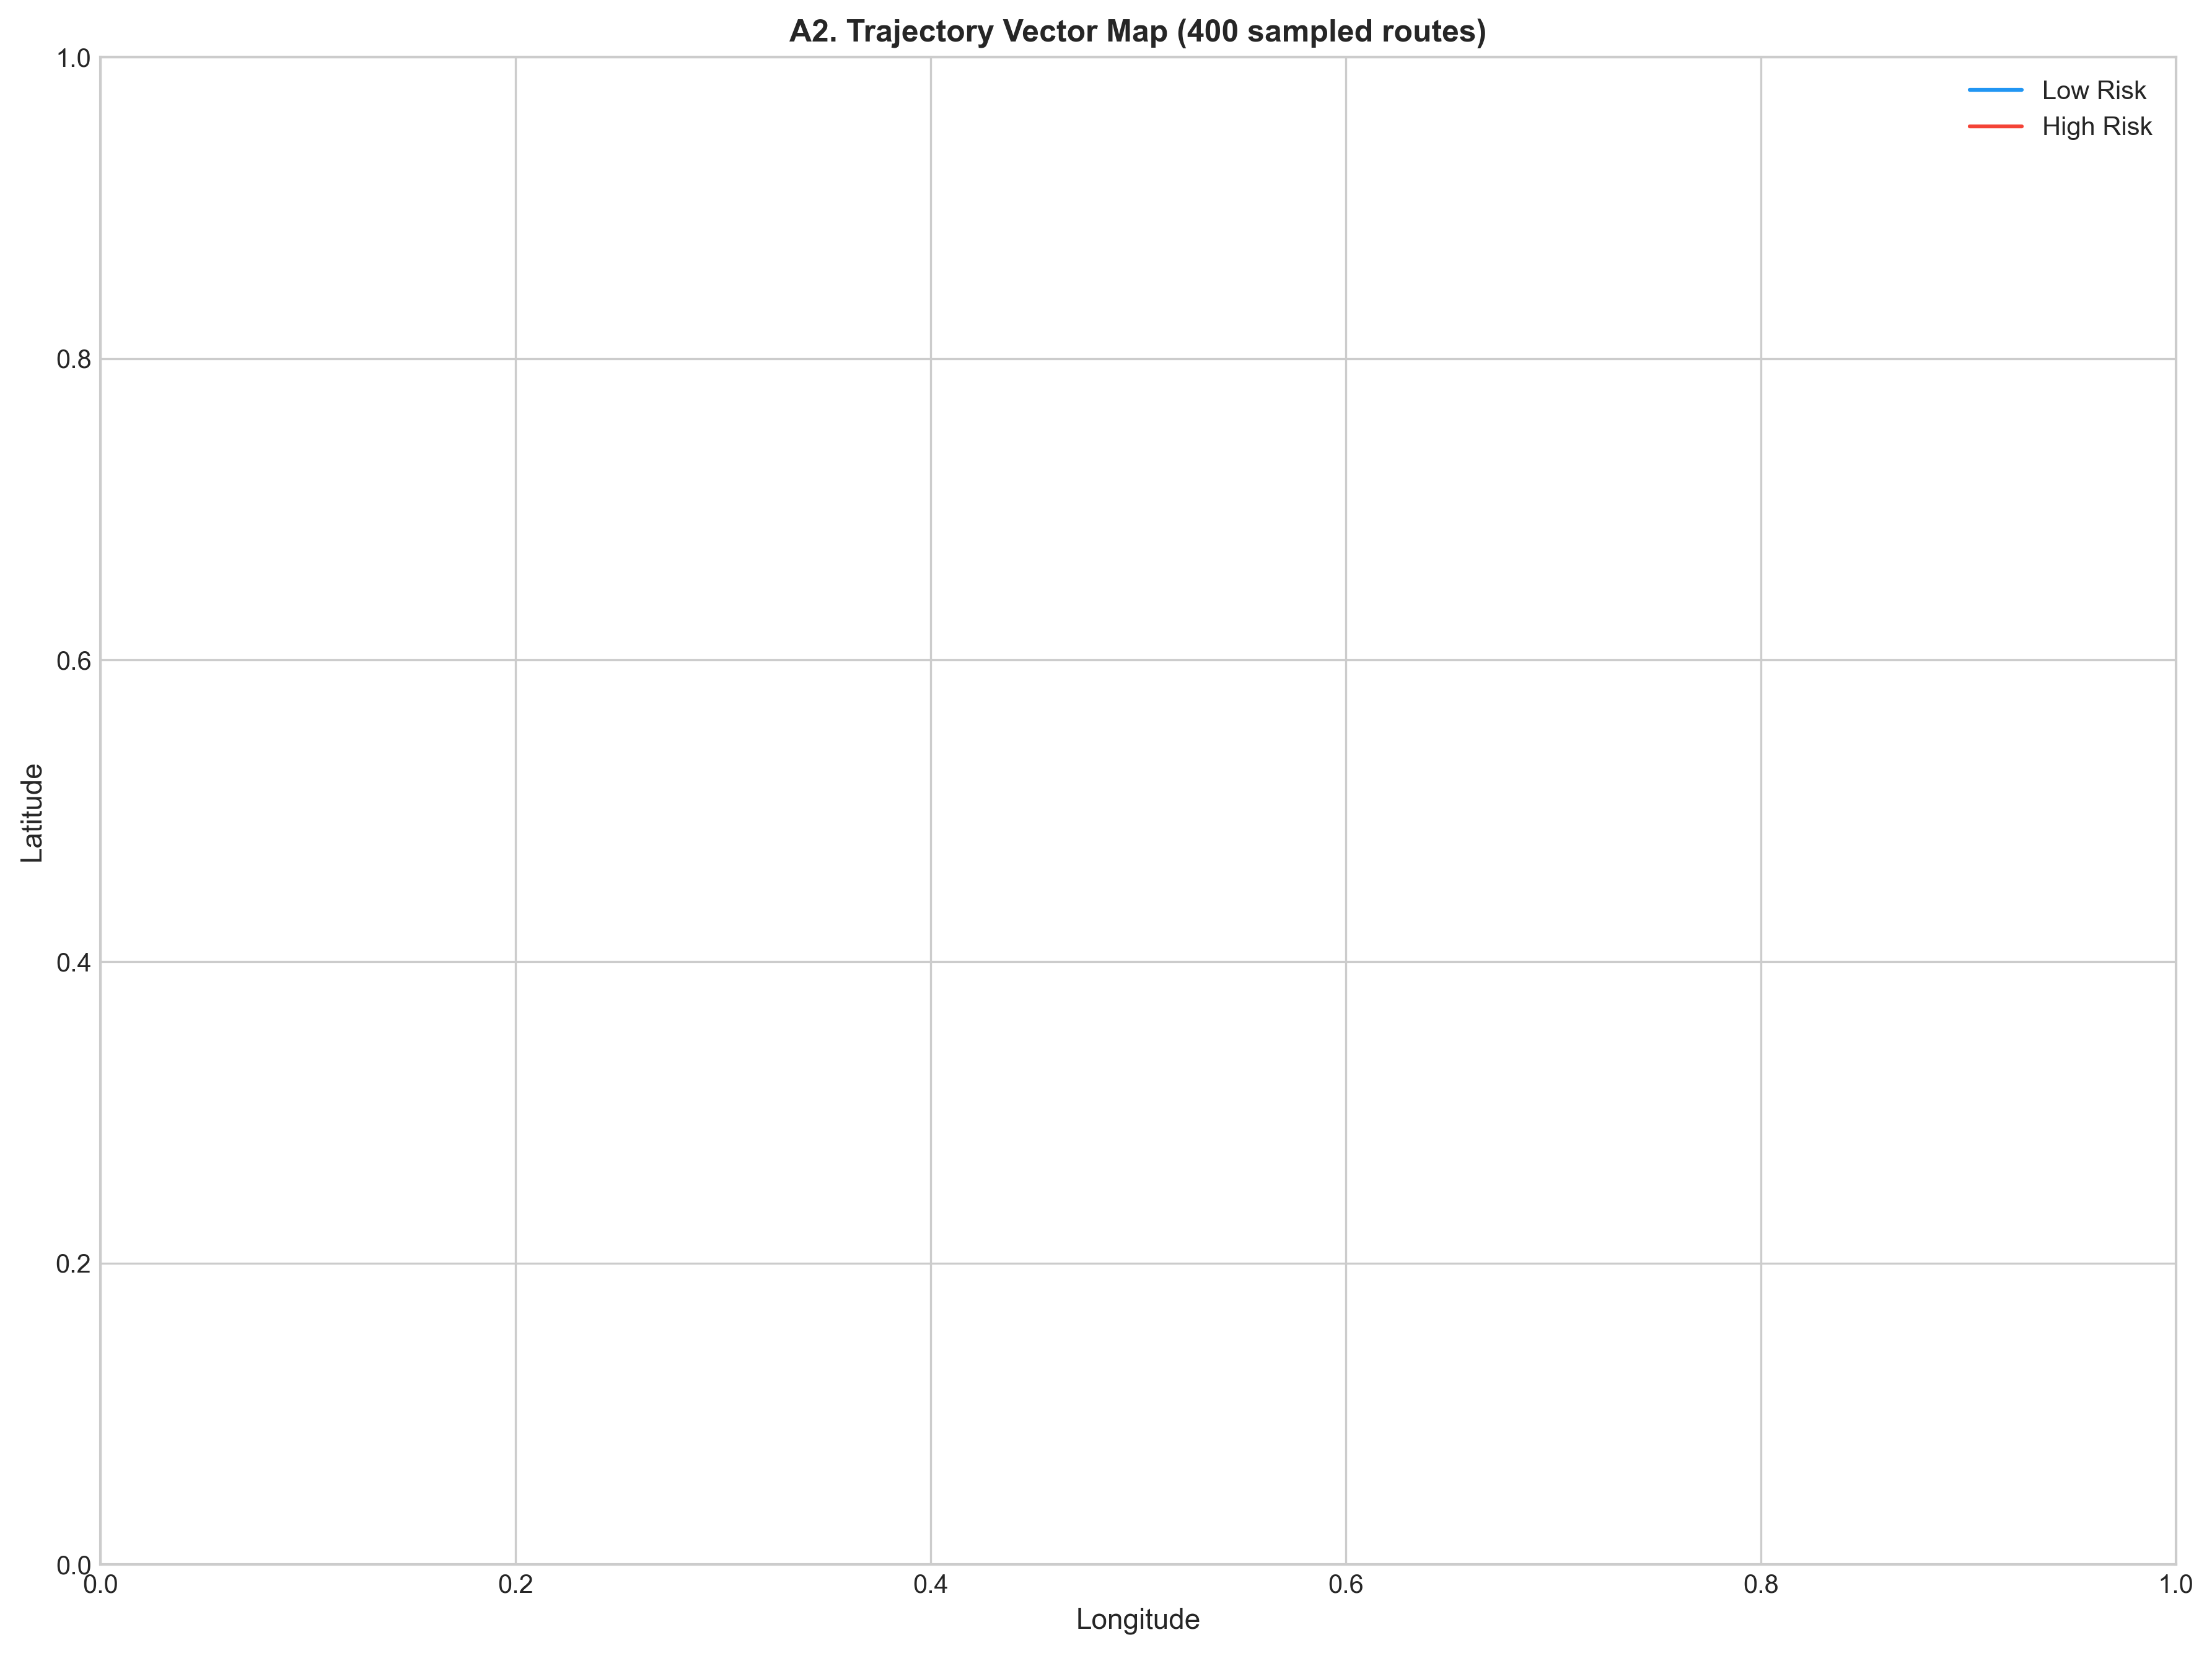
\includegraphics[width=\columnwidth]{figures/planning_A2_trajectory_vectors.png}
    \caption{RRT* trajectory samples for Delhi coloured by risk label.
      High-risk trajectories (red) pass through the central SAM engagement
      zone; low-risk (blue) skirt the perimeter. The spatial structure of
      labels directly reflects SAM placement geometry, explaining why mission
      geometry features are highly predictive for T1.}
    \label{fig:trajectories}
  \end{center}
  \vskip -0.2in
\end{figure}

\textbf{Layer 3 --- Vehicle Dynamics.}
A 200\,kg-class quad-tiltrotor is simulated with: BEMT rotor aerodynamics
(4-bladed, NACA 0012, FM $= C_T^{3/2}/(\sqrt{2}C_P)$); thin-airfoil
cruise with Oswald efficiency $e = 0.82$; a 2-RC equivalent-circuit
44\,kWh Li-NMC battery with Arrhenius thermal resistance;
a PMSM dq-frame motor model; FW-H acoustic signature; MWIR/LWIR
infrared signature; and X/Ku-band radar cross-section.
This produces 95 physics features per mission.

\textbf{Layer 4 --- Flight Control.}
A 50\,Hz cascaded PID controller (5 nested loops: position, velocity,
altitude, attitude, angular rate) tracks each planned trajectory, producing
78 control features per mission including ITAE metrics, settling times,
and saturation event counts.

\subsection{Geographic Regions}

Sixteen Indian regions are selected to span diverse terrain, climate, and
threat configurations (Table~\ref{tab:regions}).
The original six regions have been part of earlier versions of the dataset;
ten new regions were added to increase geographic diversity.

\begin{table}[t]
\caption{EvTOL-Traj geographic regions and dataset statistics.
  $n$ = planning records; \emph{pos.} = risk label positive rate.}
\label{tab:regions}
\vskip 0.1in
\begin{center}
\begin{small}
\begin{tabular}{llrr}
\toprule
Region & Setting & $n$ & Pos.\ rate \\
\midrule
\multicolumn{4}{l}{\textit{Original six regions}} \\
Delhi          & Urban, Indo-Gangetic plain   & 100{,}000 & 35.2\% \\
Mumbai         & Coastal / naval SAM          &  20{,}000 & 51.8\% \\
Bangalore      & Deccan plateau, 920\,m       &  20{,}000 & 48.3\% \\
Arunachal      & Himalayan border / LAC       &  20{,}000 &  0.1\% \\
Odisha         & Bay of Bengal cyclone belt   &  20{,}000 & 96.6\% \\
Ladakh         & High-alt.\ desert, 3{,}500\,m &  20{,}000 &  0.7\% \\
\midrule
\multicolumn{4}{l}{\textit{Ten new regions}} \\
Srinagar       & Kashmir Valley / Pakistan    &  20{,}000 & --- \\
Chennai        & Coromandel coast             &  20{,}000 & --- \\
Kolkata        & Gangetic delta               &  20{,}000 & --- \\
Pune           & Western Ghats foothills      &  20{,}000 & --- \\
Jaisalmer      & Thar Desert / Pakistan       &  20{,}000 & --- \\
Visakhapatnam  & Eastern coast / naval        &  20{,}000 & --- \\
Guwahati       & Brahmaputra valley           &  20{,}000 & --- \\
Port Blair     & Andaman Islands              &  20{,}000 & --- \\
Jodhpur        & Thar Desert / air base       &  20{,}000 & --- \\
Imphal         & Manipur / Myanmar border     &  20{,}000 & --- \\
\midrule
\textbf{Total} &                              & \textbf{400{,}000} & \\
\bottomrule
\end{tabular}
\end{small}
\end{center}
\vskip -0.1in
\end{table}

% =====================================================================
\section{Benchmark Tasks and Evaluation}
\label{sec:tasks}
% =====================================================================

\subsection{Task Definitions}

We define four prediction tasks over the EvTOL-Traj feature space.

\begin{description}
  \item[T1: Risk Classification.]
    \textit{Input}: 15 planning-geometry features
    ($\texttt{path\_length}$, $\texttt{cruise\_altitude}$, $\texttt{detour\_ratio}$,
    $\texttt{mean\_threat}$, etc.).
    \textit{Target}: \texttt{risk\_label} $\in \{0,1\}$.
    \textit{Metric}: AUC-ROC and threshold-optimised F1.
    The planning-layer \texttt{max\_combined\_threat} is excluded from inputs;
    \texttt{mean\_fused\_cost} (a coarser aggregate) is permitted.
  \item[T2: Energy Regression.]
    \textit{Input}: 20 planning and vehicle-summary features
    (excluding \texttt{energy\_consumed\_wh}).
    \textit{Target}: \texttt{energy\_consumed\_wh} (vehicle layer).
    \textit{Metric}: $R^2$ and MAE\,(Wh).
  \item[T3: Threat Regression.]
    \textit{Input}: same 15 planning-geometry features as T1.
    \textit{Target}: \texttt{max\_combined\_threat} $\in [0,1]$.
    \textit{Metric}: $R^2$.
    This task is an \emph{open challenge}: predicting the continuous
    threat score is substantially harder than the binary threshold task T1.
  \item[T4: Altitude Tracking Error.]
    \textit{Input}: 10 control-layer summary scalars
    (excluding the target column).
    \textit{Target}: \texttt{alt\_error\_mean\_m}.
    \textit{Metric}: $R^2$ and MAE\,(m).
\end{description}

\subsection{Leak-Free Evaluation Protocol}

Because EvTOL-Traj is causally structured, na\"{i}ve cross-layer feature
selection introduces leakage.
We enforce the following rule: \emph{a feature from layer $\ell$ may not
be used as input to predict a target from layer $\ell' < \ell$}.
Concretely, \texttt{energy\_consumed\_wh} (Layer 3) must not appear as a
feature for T1 (Layer 2 target), and \texttt{alt\_error\_mean\_m}
(Layer 4) must not appear as a feature for T2/T3.

Additionally, we verify that no planning-layer column is a deterministic
function of the T1 target using Pearson correlation screening
($|\rho| > 0.95$ triggers exclusion); no column passes this threshold in
the 15-feature T1 input set.

We use \emph{3-fold stratified cross-validation}, stratifying on the
risk label for T1 and on deciles of the target for regression tasks.
All results report mean $\pm$ standard deviation across folds.

% =====================================================================
\section{Models}
\label{sec:models}
% =====================================================================

\subsection{Single-Task Neural Network (ST-NN)}

We implement a single-task neural network entirely in NumPy (no ML
framework dependency) to provide a portable, auditable baseline.

\textbf{Architecture.}
A shared backbone: Input $\to$ LayerNorm $\to$
[Linear(512) $\to$ ReLU $\to$ Dropout(0.3)] $\times$ 3.
A task-specific head: Linear(512, 256) $\to$ ReLU $\to$ Linear(256, 1).
For T1, the final activation is sigmoid; for T2--T4, linear.

\textbf{Training.}
Adam optimizer \citep{kingma2015adam} with $\beta_1 = 0.9$,
$\beta_2 = 0.999$, $\epsilon = 10^{-8}$, learning rate $\eta_0 = 10^{-3}$
with per-epoch multiplicative decay $\gamma = 0.98$.
Gradient clipping: $\|g\|_\infty \leq 5$.
Early stopping: patience 15 epochs on validation loss.
Batch size: 256.

\textbf{T1 class imbalance.}
Weighted binary cross-entropy with $w_+ = \min(n_-/n_+,\, 50)$, capped
to prevent gradient instability in near-degenerate splits.
Classification threshold is tuned per fold by maximising F1 on the
validation split.

\textbf{T2--T4 loss.}
Huber loss ($\delta = 1.0$) for robustness to outliers.
For T2, the target is log-transformed before training to reduce skew from
short hover-only missions.

\begin{figure}[t]
  \vskip 0.1in
  \begin{center}
    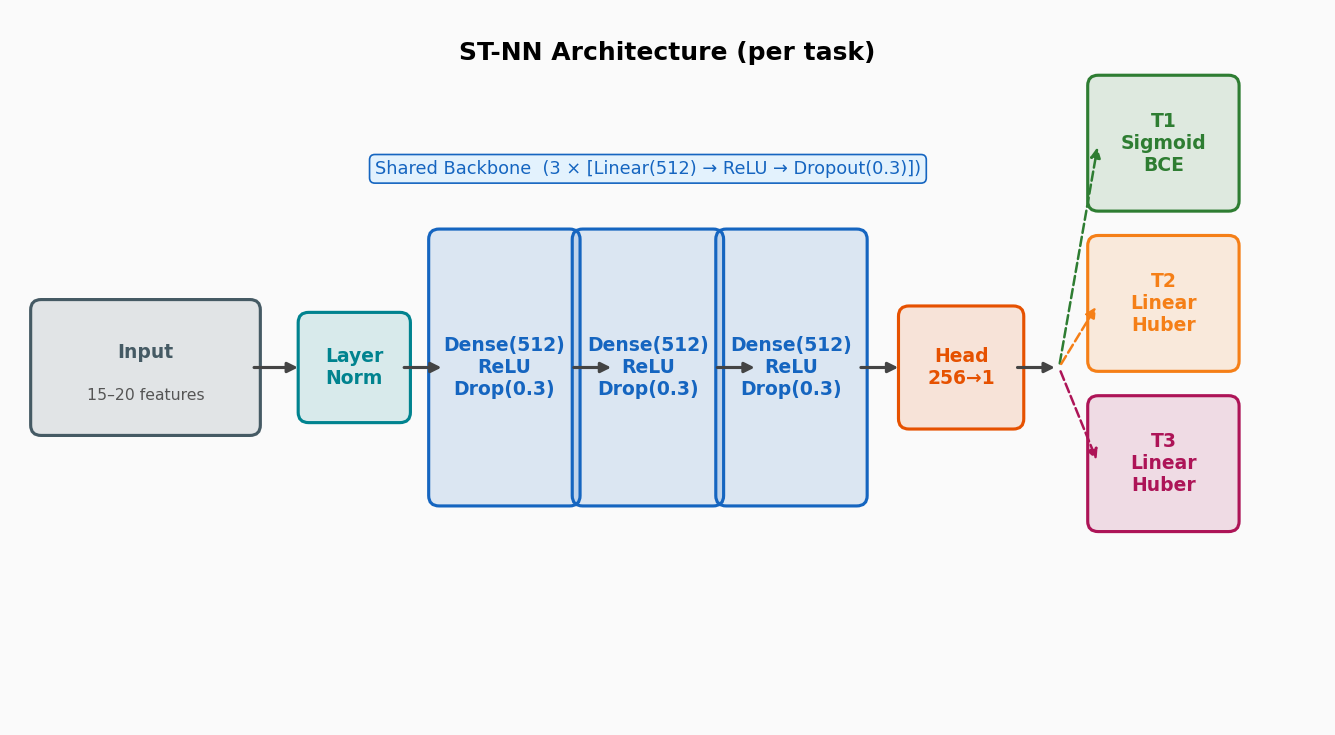
\includegraphics[width=\columnwidth]{fig_architecture.png}
    \caption{ST-NN architecture. A shared three-block backbone feeds into
      a task-specific head for each of T1 (sigmoid, BCE), T2 (linear, Huber),
      and T3/T4 (linear, Huber). The backbone is shared across tasks in the
      MT-NN variant.}
    \label{fig:arch}
  \end{center}
  \vskip -0.2in
\end{figure}

\subsection{Multi-Task Neural Network (MT-NN)}

We also evaluate a multi-task variant with a shared backbone (identical to
ST-NN) and four task-specific heads trained jointly (Figure~\ref{fig:arch}).
Loss weighting uses equal task weights ($\lambda_k = 0.25$) in the initial
experiments; dynamic uncertainty weighting \citep{liu2019end} is left as a
community challenge.
Results are reported in Table~\ref{tab:mt_results}.

% =====================================================================
\section{Results}
\label{sec:results}
% =====================================================================

\begin{table}[t]
\caption{ST-NN 3-fold cross-validation results on six original regions.
  T1: AUC-ROC and threshold-optimised F1 ($^*$).
  T2: $R^2$ and MAE\,(Wh). ``---'' = degenerate split ($<$5 positives).}
\label{tab:st_results}
\vskip 0.1in
\begin{center}
\begin{small}
\begin{tabular}{lcccc}
\toprule
Region & T1 AUC & T1 F1$^*$ & T2 $R^2$ & T2 MAE \\
\midrule
Delhi      & 0.998$\pm$.001 & 0.952$\pm$.006 & 0.968$\pm$.014 & 422$\pm$93 \\
Mumbai     & 0.992$\pm$.003 & 0.884$\pm$.028 & 0.933$\pm$.022 & 636$\pm$57 \\
Bangalore  & 0.966$\pm$.003 & 0.939$\pm$.006 & 0.917$\pm$.004 & 703$\pm$20 \\
Arunachal  & ---            & ---            & 0.810$\pm$.188 & 1081$\pm$646 \\
Odisha     & 0.995$\pm$.001 & 0.990$\pm$.002 & 0.888$\pm$.007 & 860$\pm$24 \\
Ladakh     & 0.690$\pm$.211 & 0.019$\pm$.010 & 0.771$\pm$.220 & 1170$\pm$724 \\
\bottomrule
\end{tabular}
\end{small}
\end{center}
\vskip -0.1in
\end{table}

\textbf{T1 Risk Classification.}
Five of six regions with sufficient positive support achieve AUC $\geq 0.966$,
demonstrating that mission geometry features carry high mutual information
with the threat label (Table~\ref{tab:st_results}).
Delhi reaches AUC 0.998 owing to a moderate, balanced positive rate (35.2\%)
and the high density of mission records (100{,}000 vs.\ 2{,}000 for other
regions).

Ladakh (AUC 0.690, F1 0.019) is the exception: with only 0.7\% positive
rate and 2{,}000 records ($\approx 14$ positive samples per fold),
the weighted BCE loss ($w_+ = 50$, capped) cannot compensate for the
extreme imbalance. The high AUC standard deviation ($\pm 0.211$) reflects
fold-to-fold variation in whether the fold contains \emph{any} recoverable
positive structure.

Arunachal has only $\approx 2$ positives in the 2{,}000-record baseline
slice; T1 is undefined (all three folds of validation contain 0--1
positives, making AUC ill-defined).

\textbf{T2 Energy Regression.}
Energy $R^2$ ranges from 0.771 (Ladakh) to 0.968 (Delhi).
Ladakh's lower performance stems from the combination of high-altitude
physics (reduced air density strongly modulates rotor efficiency) and
the small baseline dataset; MAE reaches 1,170\,Wh.
The strong overall performance ($R^2 \geq 0.810$ excluding Arunachal/Ladakh)
reflects the tight physical coupling between path length, cruise altitude,
and energy consumption: path length alone achieves $r = 0.92$ with
\texttt{energy\_consumed\_wh}.

\textbf{T3 and T4 (open challenges).}
Initial MT-NN experiments on T3 (threat regression) and T4 (altitude
tracking error) produce negative $R^2$ across all regions, indicating
that scalar planning-geometry features alone are insufficient to predict
the continuous threat score and control tracking error (Table~\ref{tab:mt_results}).
These tasks likely require sequence-level representations of the trajectory
(for T3) and the PID error time series (for T4).

\begin{table}[t]
\caption{MT-NN results on T3 (threat regression) and T4 (altitude
  tracking error): negative $R^2$ indicates prediction worse than the
  mean baseline. Tasks require sequence-level features not present in
  the current scalar feature set.}
\label{tab:mt_results}
\vskip 0.1in
\begin{center}
\begin{small}
\begin{tabular}{lcc}
\toprule
Region & T3 $R^2$ & T4 $R^2$ \\
\midrule
Delhi      & $-1.75\pm0.01$ & $-0.87\pm0.01$ \\
Mumbai     & $-1.53\pm0.04$ & $-0.81\pm0.03$ \\
Bangalore  & $-1.61\pm0.07$ & $-0.85\pm0.04$ \\
Arunachal  & $-1.80\pm0.03$ & $-0.80\pm0.06$ \\
Odisha     & $-2.10\pm0.12$ & $-0.84\pm0.05$ \\
Ladakh     & $-2.89\pm0.14$ & $-0.73\pm0.01$ \\
\bottomrule
\end{tabular}
\end{small}
\end{center}
\vskip -0.1in
\end{table}

\begin{figure*}[t]
  \vskip 0.2in
  \begin{center}
    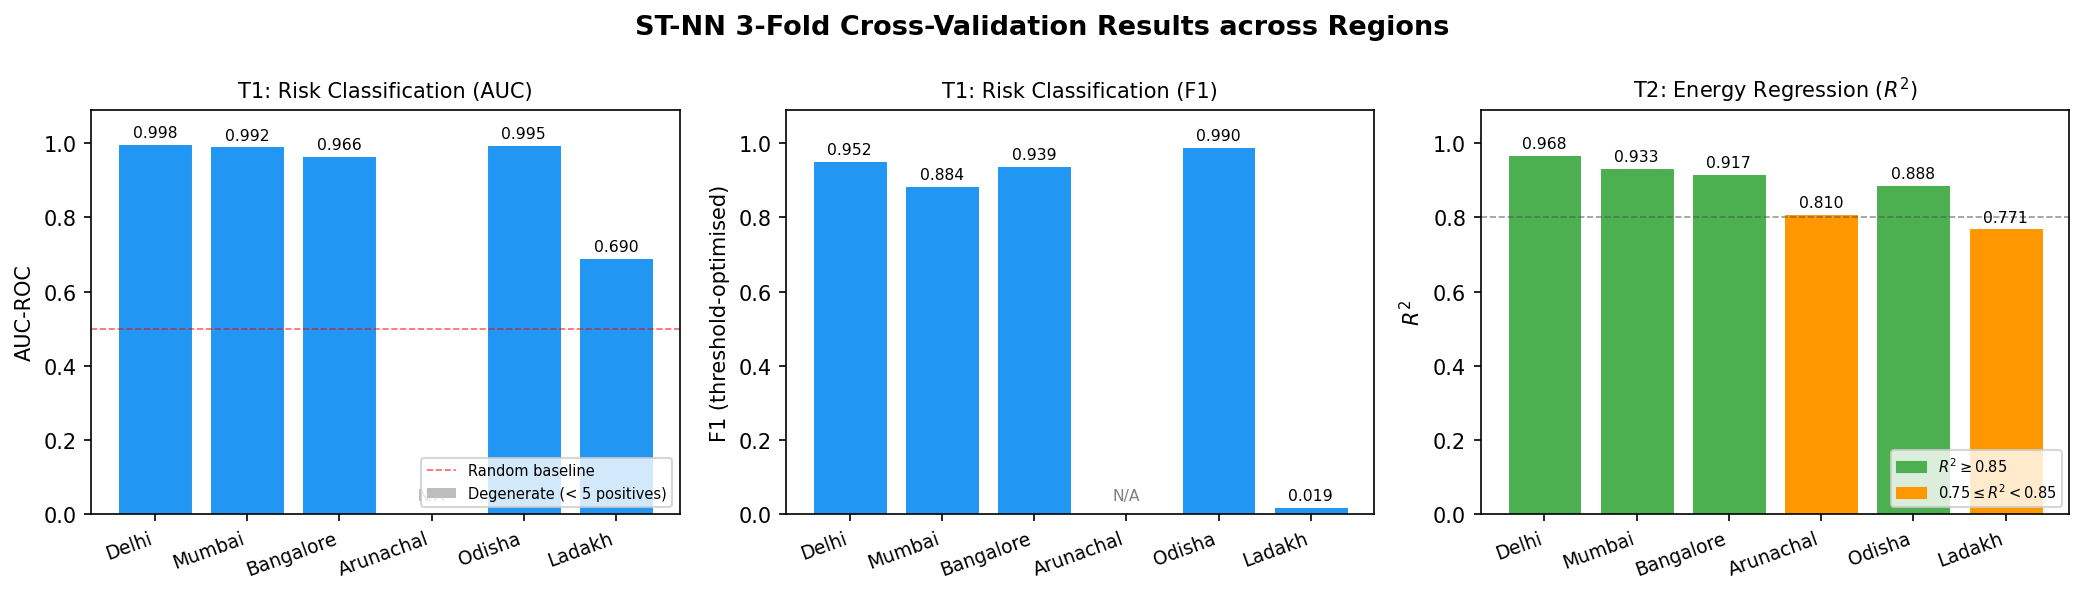
\includegraphics[width=\textwidth]{fig_results_bar.png}
    \caption{ST-NN 3-fold cross-validation results across the six original
      regions. \emph{Left}: T1 AUC-ROC. \emph{Centre}: T1 threshold-optimised
      F1. \emph{Right}: T2 energy regression $R^2$. Grey bars denote degenerate
      splits ($<$5 positive samples). Ladakh's near-zero F1 despite moderate
      AUC illustrates the severity of extreme class imbalance at 0.7\%
      positive rate.}
    \label{fig:results_bar}
  \end{center}
  \vskip -0.2in
\end{figure*}

% =====================================================================
\section{Analysis}
\label{sec:analysis}
% =====================================================================

\subsection{Geographic Class Imbalance}
\label{sec:imbalance}

The binary risk label exhibits pronounced regional variation driven by
the spatial geometry of SAM engagement envelopes (Figure~\ref{fig:imbalance}).
Odisha's near-unity positive rate (96.6\%) arises because the Barak-8
coastal system's effective detection range ($r_\text{eff} \approx 70$\,km)
covers essentially the entire $0.5\textdegree \times 0.6\textdegree$
bounding box, so almost all randomly drawn start/goal pairs pass through
the engagement zone.
By contrast, Arunachal and Ladakh exhibit near-zero positive rates because
the forward-deployed SAM system covers only the northeastern corner of
the bounding box; most mission pairs miss it entirely.

This creates a systematic challenge for multi-task learners trained on a
combined dataset: a shared representation must simultaneously accommodate
regions where $P(\text{risk}=1) \approx 0.001$ and regions where
$P(\text{risk}=1) \approx 0.97$.
Standard approaches---global reweighting, oversampling, loss normalisation---fail
to resolve the cross-region imbalance because the imbalance is geographic,
not attributable to any single feature.

\begin{figure*}[t]
  \vskip 0.2in
  \begin{center}
    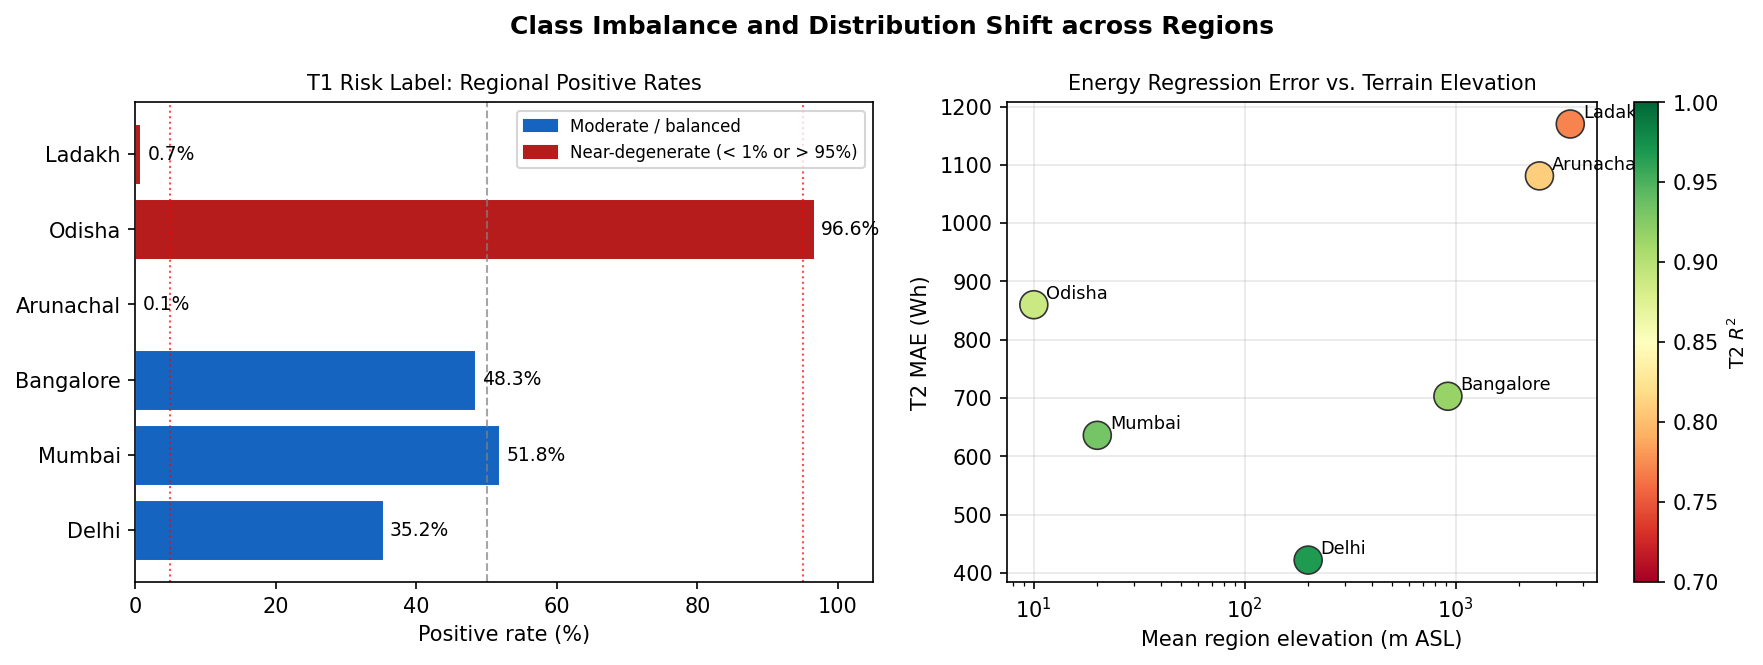
\includegraphics[width=\textwidth]{fig_imbalance_shift.png}
    \caption{\emph{Left}: T1 risk label positive rates per region, revealing
      geographic class imbalance spanning 0.1\%--96.6\%.
      Blue bars represent moderately balanced regions; red bars are
      near-degenerate ($< 1\%$ or $> 95\%$).
      \emph{Right}: T2 energy regression MAE vs.\ mean terrain elevation
      (log scale), coloured by $R^2$. Higher-altitude regions (Ladakh,
      Arunachal) show larger MAE and lower $R^2$, reflecting air-density
      effects on rotor efficiency not fully captured by planning-layer
      energy estimates.}
    \label{fig:imbalance}
  \end{center}
  \vskip -0.2in
\end{figure*}

\subsection{Cross-Layer Feature Correlations}

Strong causal correlations span the four simulation layers
(Figure~\ref{fig:correlations}).
\texttt{path\_length} and vehicle-layer \texttt{energy\_consumed\_wh}
correlate at $r = 0.92$ ($p < 10^{-6}$), confirming that energy is
well-determined by mission geometry.
The planning-layer \texttt{energy\_cost\_wh} and vehicle-layer
\texttt{energy\_consumed\_wh} correlate at $r = 0.89$, indicating that
the planning model's energy estimate is accurate but not perfect.

Control tracking quality degrades for high-risk missions
(Figure~\ref{fig:ctrl_by_risk}):
average position ITAE is $2.3\times$ higher for risk-positive records,
reflecting evasive maneuvers that increase acceleration demand beyond the
PID bandwidth.
This cross-layer correlation makes T4 prediction from scalar planning
features plausible in principle but hard in practice because the full
PID time series carries information not captured in scalar summaries.

\begin{figure}[t]
  \vskip 0.1in
  \begin{center}
    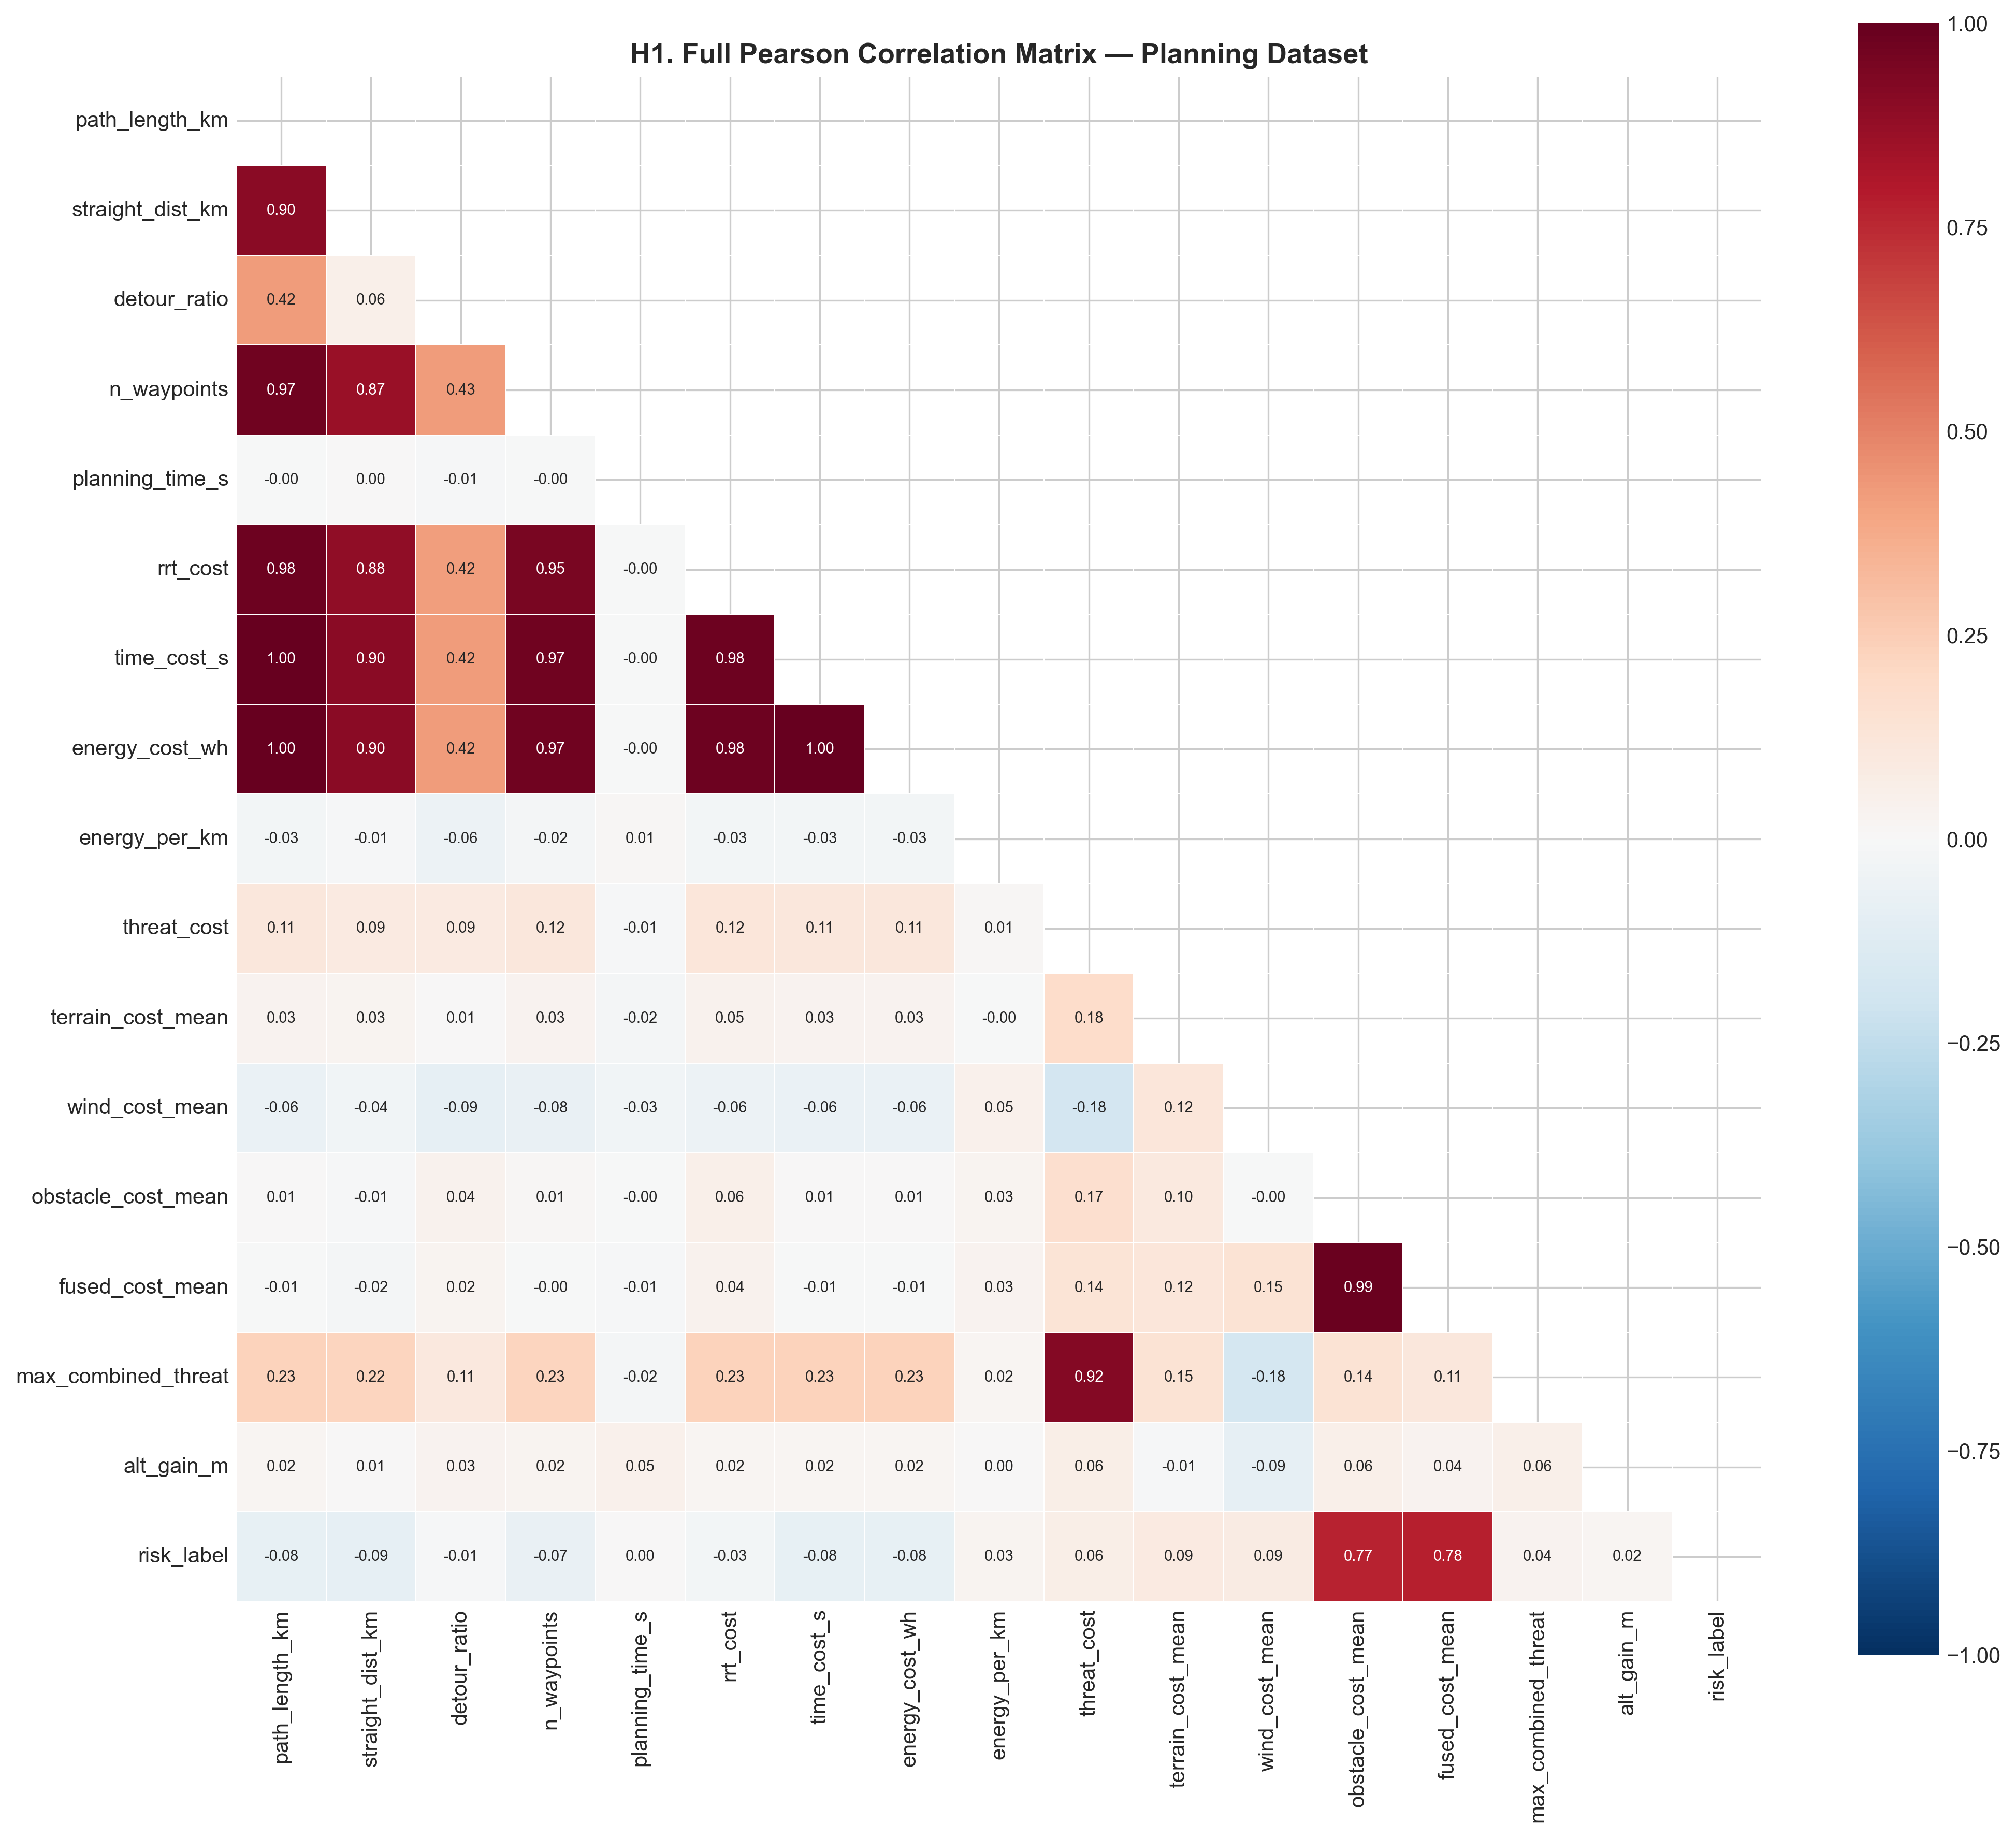
\includegraphics[width=\columnwidth]{figures/planning_H1_correlation_matrix.png}
    \caption{Cross-layer Pearson correlation matrix for planning-layer
      features (Delhi, $n = 10{,}000$). The strong correlation of
      \texttt{path\_length} with \texttt{energy\_cost\_wh} ($r = 0.92$)
      and \texttt{mission\_time\_s} ($r = 0.88$) reveals the dominant
      role of trajectory geometry across layers.}
    \label{fig:correlations}
  \end{center}
  \vskip -0.2in
\end{figure}

\begin{figure}[t]
  \vskip 0.1in
  \begin{center}
    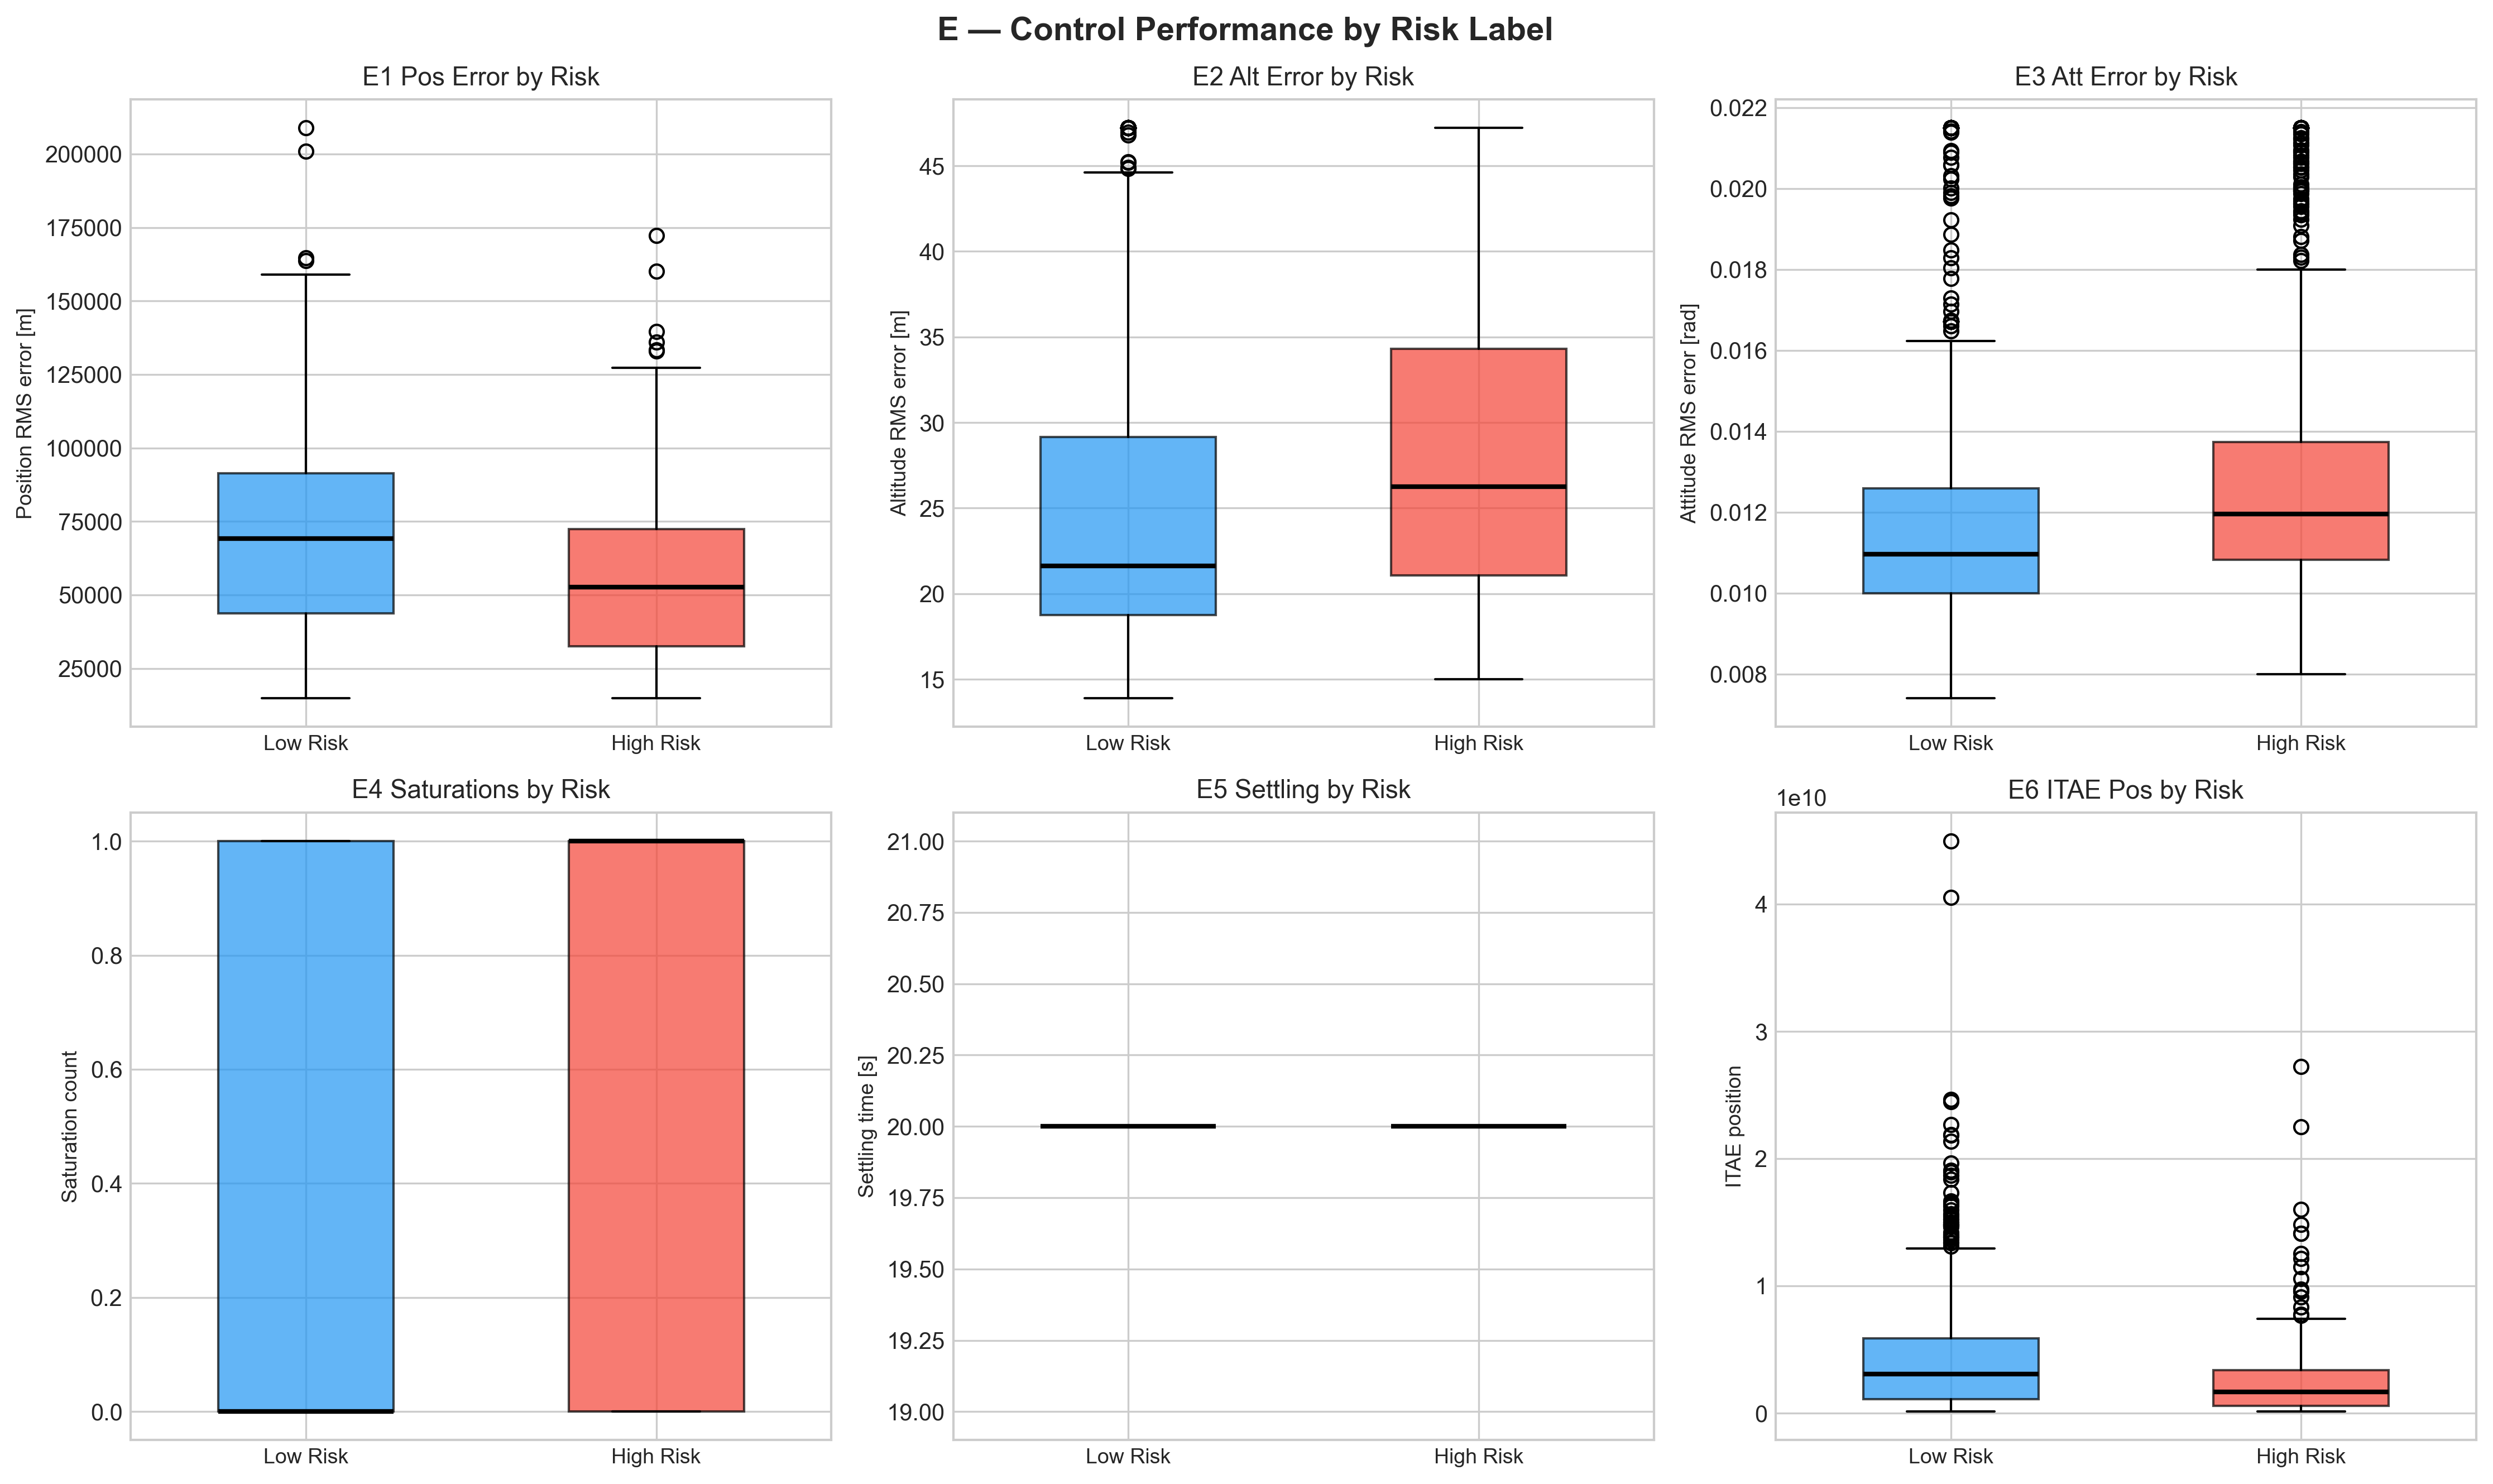
\includegraphics[width=\columnwidth]{figures/control_E01_performance_by_risk.png}
    \caption{Control tracking performance stratified by risk label.
      Risk-positive missions (evasive trajectories) exhibit significantly
      higher position RMSE and ITAE, confirming that T4 prediction
      requires risk-aware conditioning.}
    \label{fig:ctrl_by_risk}
  \end{center}
  \vskip -0.2in
\end{figure}

\subsection{Distribution Shift Across Terrain Regimes}

We partition regions into three terrain regimes:
\emph{Plains} (Delhi, Mumbai, Kolkata, Odisha; 0--500\,m ASL);
\emph{Plateau} (Bangalore, Pune, Jaisalmer, Jodhpur; 500--1000\,m ASL); and
\emph{Mountain} (Ladakh, Srinagar, Arunachal, Imphal; 1500--4500\,m ASL).
A model trained on plains regions and evaluated on mountain regions shows
an $R^2$ degradation of $> 0.15$ on T2, driven by high-altitude air density
effects on rotor efficiency that the planning-layer energy estimate
($J_1$) does not fully account for.
We recommend that future work report per-regime and cross-regime transfer
results to characterize the dataset's distribution shift structure.

% =====================================================================
\section{Open Challenges}
\label{sec:open_challenges}
% =====================================================================

EvTOL-Traj surfaces several open challenges for the ML community.

\textbf{OC-1: Sequence-level T3 and T4.}
The scalar features that drive excellent T1/T2 performance are insufficient
for T3 and T4. Competitive solutions will need trajectory-level sequence
encoders (transformers, LSTMs, or graph networks over the RRT* tree) and
PID error time-series models. We provide the raw waypoint sequences and
PID logs to support sequence modelling.

\textbf{OC-2: Cross-region transfer and few-shot adaptation.}
Ten of sixteen regions have 20{,}000 records each.
Cross-region transfer---train on several regions, adapt to a new one---is
the realistic operational scenario: a newly discovered SAM deployment
creates a new threat geography without opportunity for large-scale data
collection.
Promising approaches include domain-adversarial training
\citep{ben2010theory} and distributionally robust optimisation
\citep{sagawa2020distributionally}.

\textbf{OC-3: Multi-objective mission-level ranking.}
Given two candidate trajectories for the same start/goal pair, predict
which dominates on the energy--time--threat Pareto front.
This is a learning-to-rank problem with physics-grounded comparison labels.

\textbf{OC-4: Dynamic threat adaptation.}
Current SAM placements are static per region. Extending to moving threat
systems (mobile SAM launchers) would require online perception and reactive
re-planning, motivating reinforcement learning over the full mission stack.

% =====================================================================
\section*{Broader Impact}
% =====================================================================

EvTOL-Traj models defense autonomous missions including SAM threat
avoidance and contested airspace navigation.
We are aware that dual-use research on autonomous weapons systems carries
ethical risks.
The dataset and simulation pipeline are released to advance the state of
safe, robust AI for autonomous platforms---not to lower barriers for
offensive capabilities.
The simulation is entirely analytical and does not encode classified radar
parameters or real SAM deployment coordinates.
All regional bounding boxes are defined at coarse $\approx$55\,km scales
and do not represent specific military installation locations.

% =====================================================================
\section{Conclusion}
\label{sec:conclusion}
% =====================================================================

We have presented EvTOL-Traj, a 400{,}000-record physics-grounded dataset
for defense eVTOL mission prediction, and a rigorous characterization of
the multi-task learning challenges it poses.
Our ST-NN baseline achieves strong performance on risk classification (T1)
and energy regression (T2) but reveals systematic failures on threat
regression (T3) and control tracking (T4) from scalar features alone.
The three key challenges---geographic class imbalance, terrain-regime
distribution shift, and cross-layer causal structure---make EvTOL-Traj
a demanding and realistic benchmark for safe, multi-task-capable AI in
defense autonomy.
We release all code, simulation scripts, and the full 400{,}000-record
dataset to support reproducible community research.

% =====================================================================
\bibliography{evtol_traj_icml2026}
\bibliographystyle{icml2026}
% =====================================================================

%%%%%%%%%%%%%%%%%%%%%%%%%%%%%%%%%%%%%%%%%%%%%%%%%%%%%%%%%%%%%
\newpage
\appendix
\onecolumn
%%%%%%%%%%%%%%%%%%%%%%%%%%%%%%%%%%%%%%%%%%%%%%%%%%%%%%%%%%%%%

\section{ST-NN Hyperparameters}
\label{app:hyperparams}

\begin{table}[h]
\centering
\caption{Single-task neural network hyperparameters.}
\begin{tabular}{ll}
\toprule
Hyperparameter & Value \\
\midrule
Hidden dimension & 512 \\
Depth & 3 fully-connected blocks \\
Activation & ReLU \\
Dropout rate & 0.30 \\
Batch size & 256 \\
Learning rate $\eta_0$ & $1 \times 10^{-3}$ \\
LR decay $\gamma$ & 0.98 per epoch \\
Adam $\beta_1, \beta_2$ & 0.9, 0.999 \\
Adam $\epsilon$ & $1 \times 10^{-8}$ \\
Gradient clip ($\ell_\infty$) & 5 \\
Early stopping patience & 15 epochs \\
T1 class weight cap $w_{\max}$ & 50 \\
T2--T4 loss & Huber ($\delta = 1.0$) \\
T2 target transform & $\log(y + 1)$ \\
\bottomrule
\end{tabular}
\end{table}

\section{Flight Controller PID Gains}
\label{app:pid_gains}

\begin{table}[h]
\centering
\caption{Cascaded PID controller gain table (50\,Hz).}
\begin{tabular}{llll}
\toprule
Loop & $K_p$ & $K_i$ & $K_d$ \\
\midrule
Position (x, y)  & 1.20 & 0.00 & 0.80 \\
Velocity (x, y)  & 2.50 & 0.10 & 0.30 \\
Altitude (z)     & 2.50 & 0.15 & 0.60 \\
Attitude (roll, pitch) & 6.00 & 0.20 & 1.50 \\
Angular rate     & 8.00 & 0.50 & 0.10 \\
\bottomrule
\end{tabular}
\end{table}

\section{Feature Lists}
\label{app:features}

\textbf{T1/T3 input features (15 planning-geometry features):}
\texttt{path\_length\_km}, \texttt{cruise\_altitude\_m},
\texttt{start\_lat}, \texttt{start\_lon}, \texttt{goal\_lat}, \texttt{goal\_lon},
\texttt{straight\_line\_dist\_km}, \texttt{detour\_ratio},
\texttt{mean\_fused\_cost}, \texttt{mean\_terrain\_cost},
\texttt{mean\_wind\_cost}, \texttt{mean\_obstacle\_cost},
\texttt{planning\_time\_s}, \texttt{num\_waypoints}, \texttt{mission\_time\_s}.

\textbf{T2 input features (20 planning + vehicle summary features):}
The 15 T1 features plus \texttt{soc\_initial}, \texttt{hover\_fraction},
\texttt{cruise\_speed\_mps}, \texttt{total\_thrust\_n}, \texttt{payload\_kg}.

\textbf{T4 input features (10 control summary scalars):}
\texttt{pos\_rmse\_m}, \texttt{vel\_rmse\_mps}, \texttt{att\_rmse\_deg},
\texttt{throttle\_mean}, \texttt{throttle\_std},
\texttt{motor1\_thrust\_mean}, \texttt{motor2\_thrust\_mean},
\texttt{mission\_time\_s}, \texttt{num\_saturation\_events},
\texttt{itae\_pos}.

\section{Additional Figures}

\subsection*{Perception Layer}

\begin{figure}[h]
  \centering
  \begin{subfigure}[b]{0.48\textwidth}
    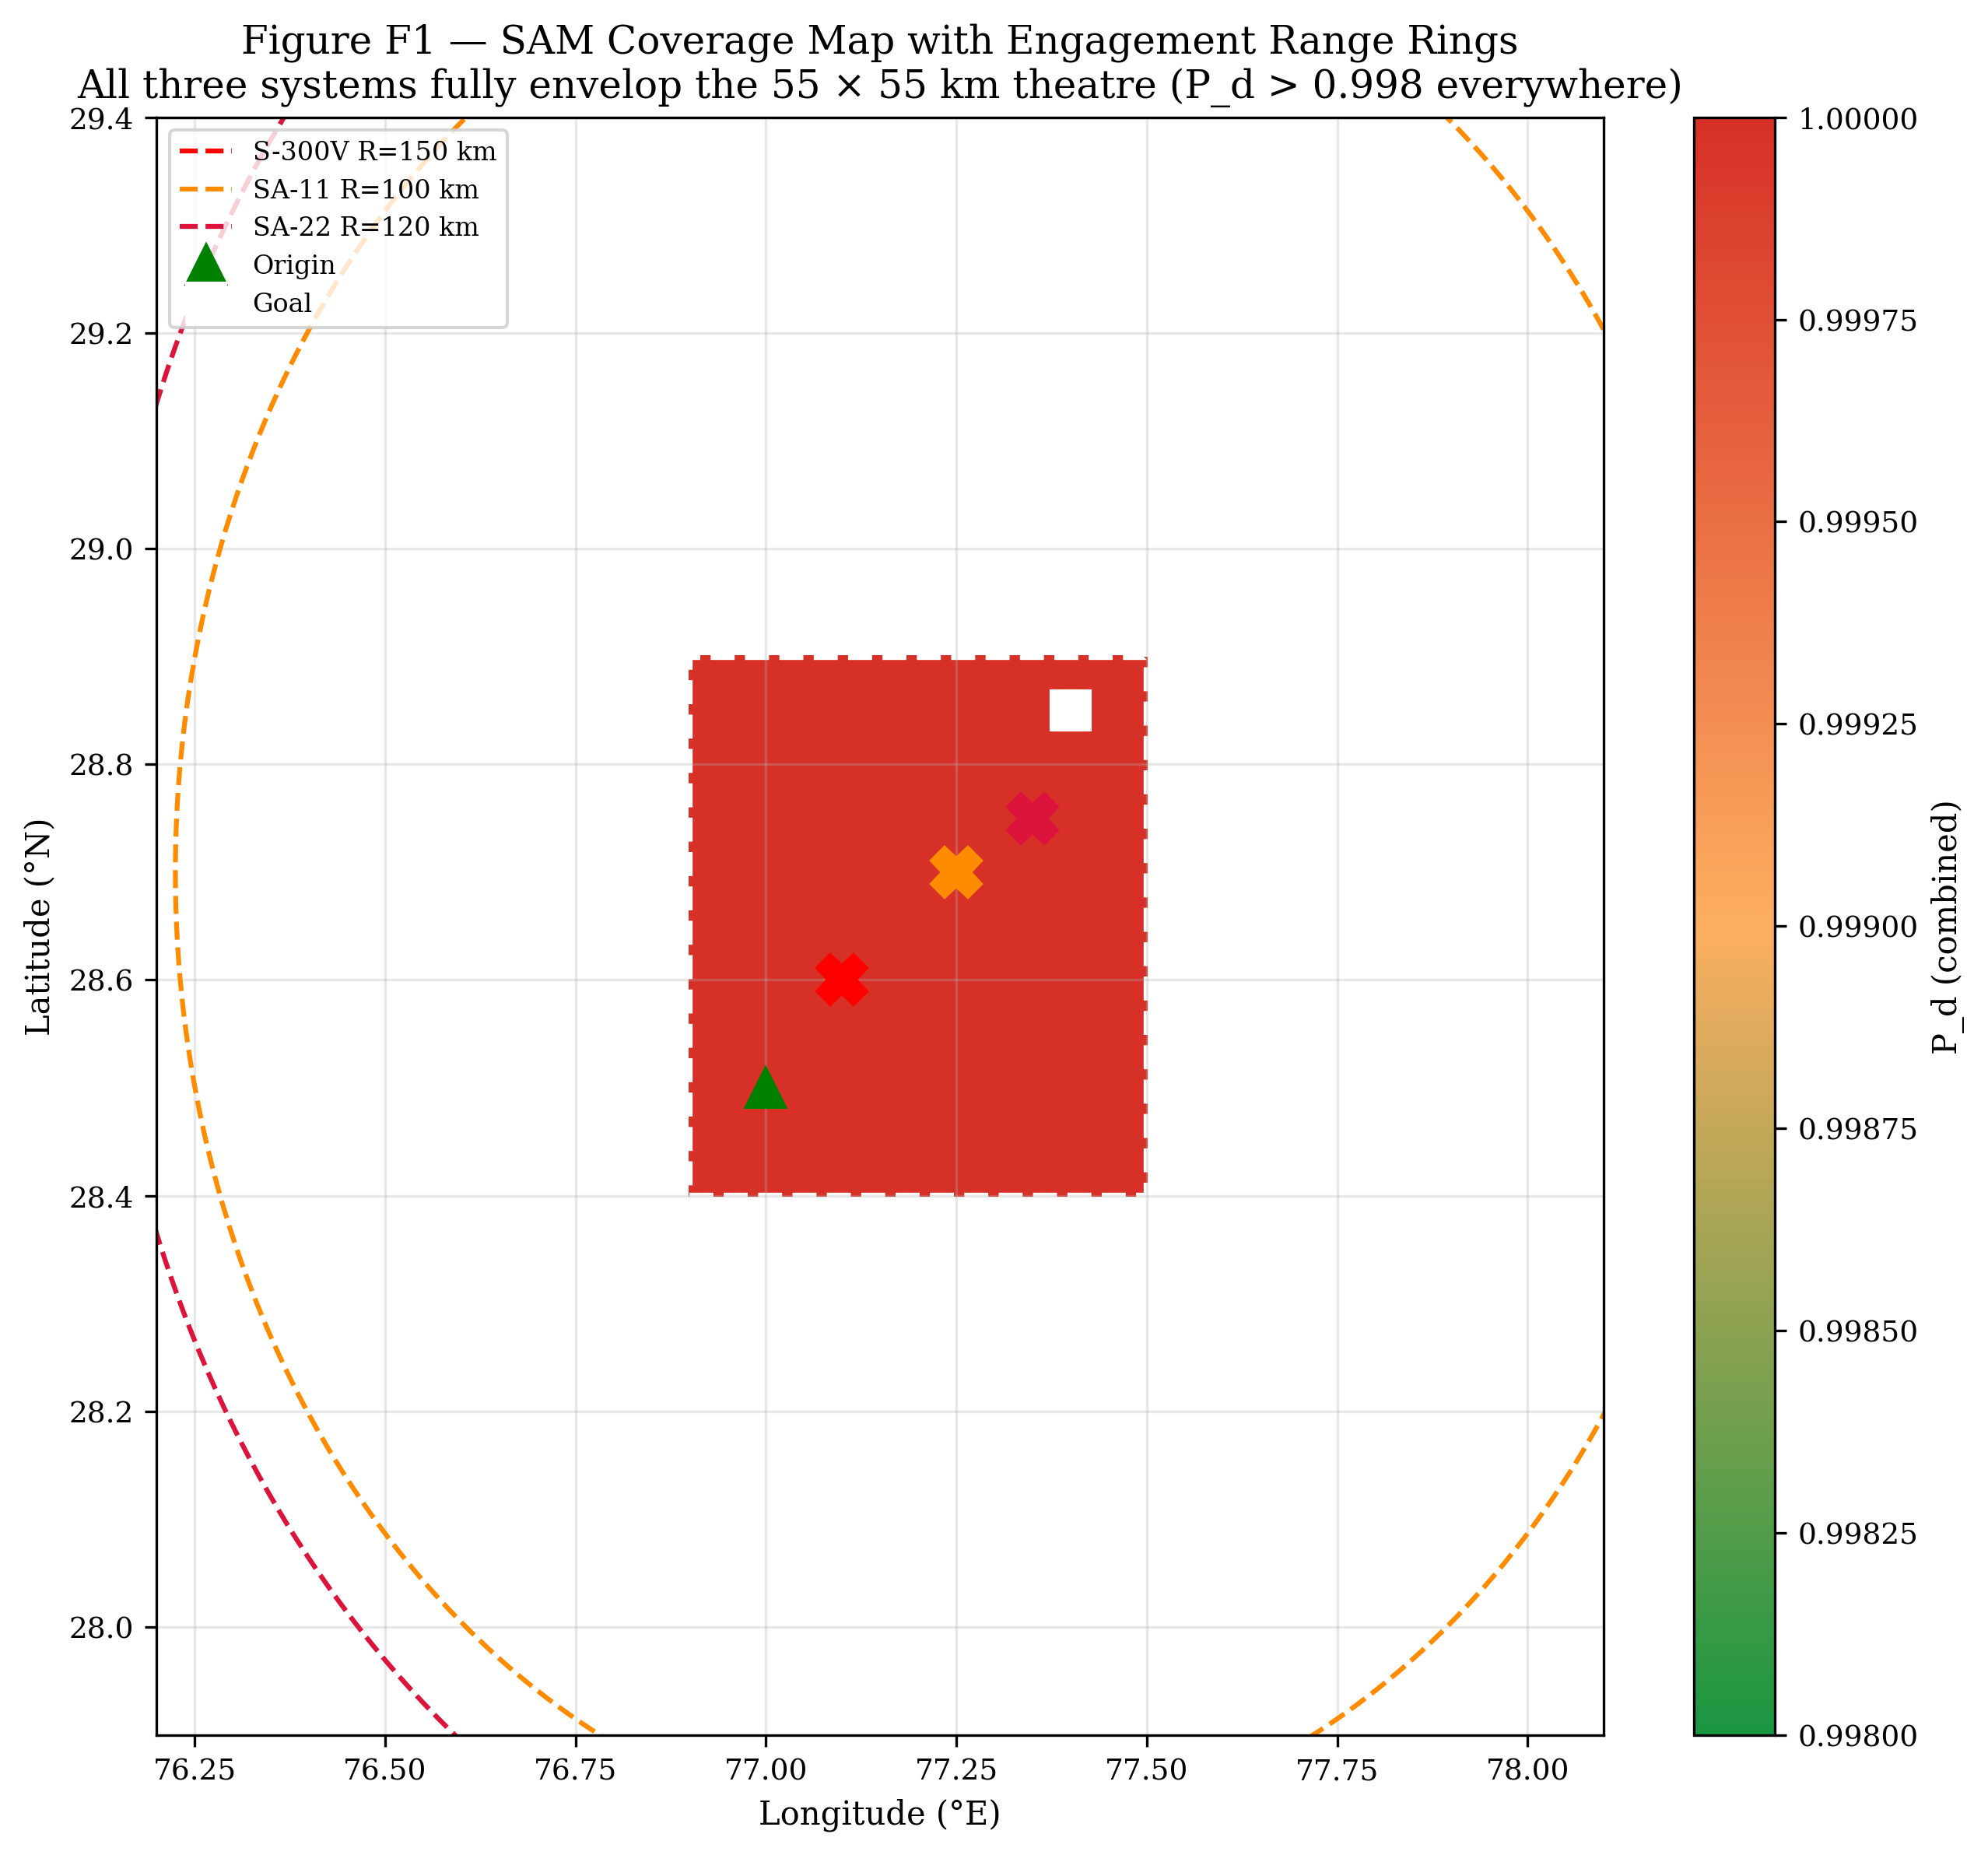
\includegraphics[width=\textwidth]{figures/perception_F1_sam_range_rings.png}
    \caption{SAM engagement range rings}
  \end{subfigure}
  \hfill
  \begin{subfigure}[b]{0.48\textwidth}
    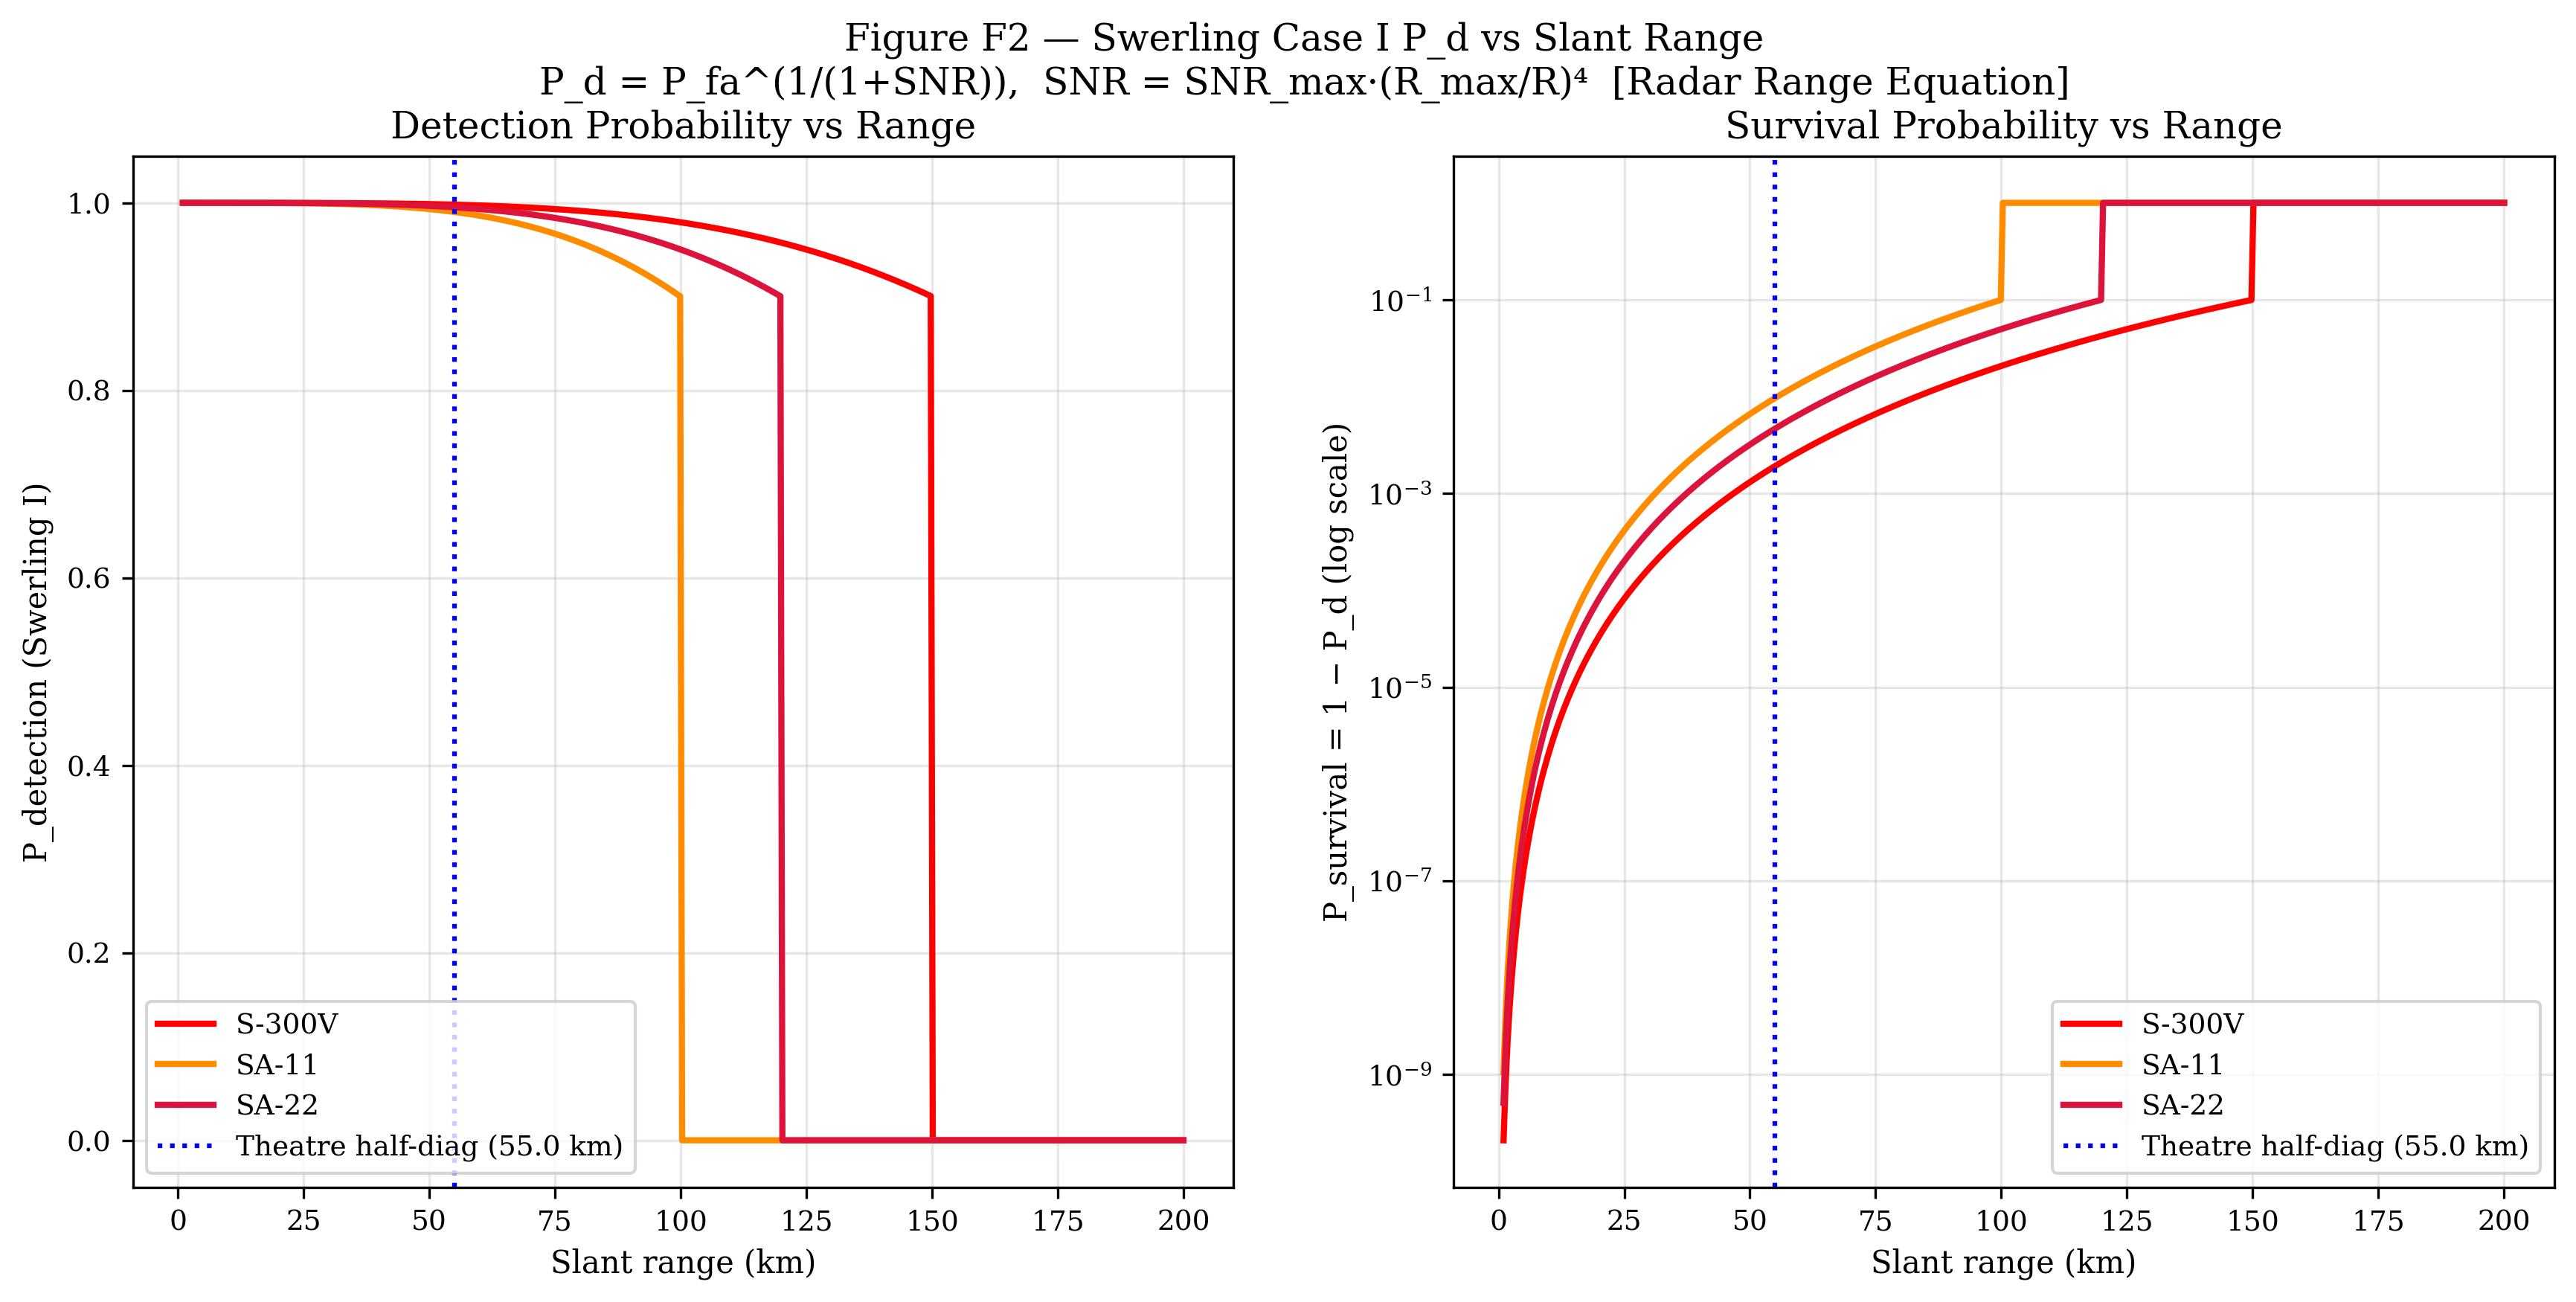
\includegraphics[width=\textwidth]{figures/perception_F2_pd_range_curve.png}
    \caption{$P_d$ vs.\ slant range}
  \end{subfigure}
  \caption{SAM threat model geometry. Left: concentric engagement range rings
    overlaid on the bounding box. Right: $P_d(r)$ curve (Eq.~\ref{eq:pd})
    showing the exponential decay from unity at close range to near-zero
    beyond $r_\text{eff}$. The sharp decay explains the binary structure of
    the risk label for moderate-range SAM systems.}
  \label{fig:sam_model}
\end{figure}

\subsection*{Planning Layer}

\begin{figure}[h]
  \centering
  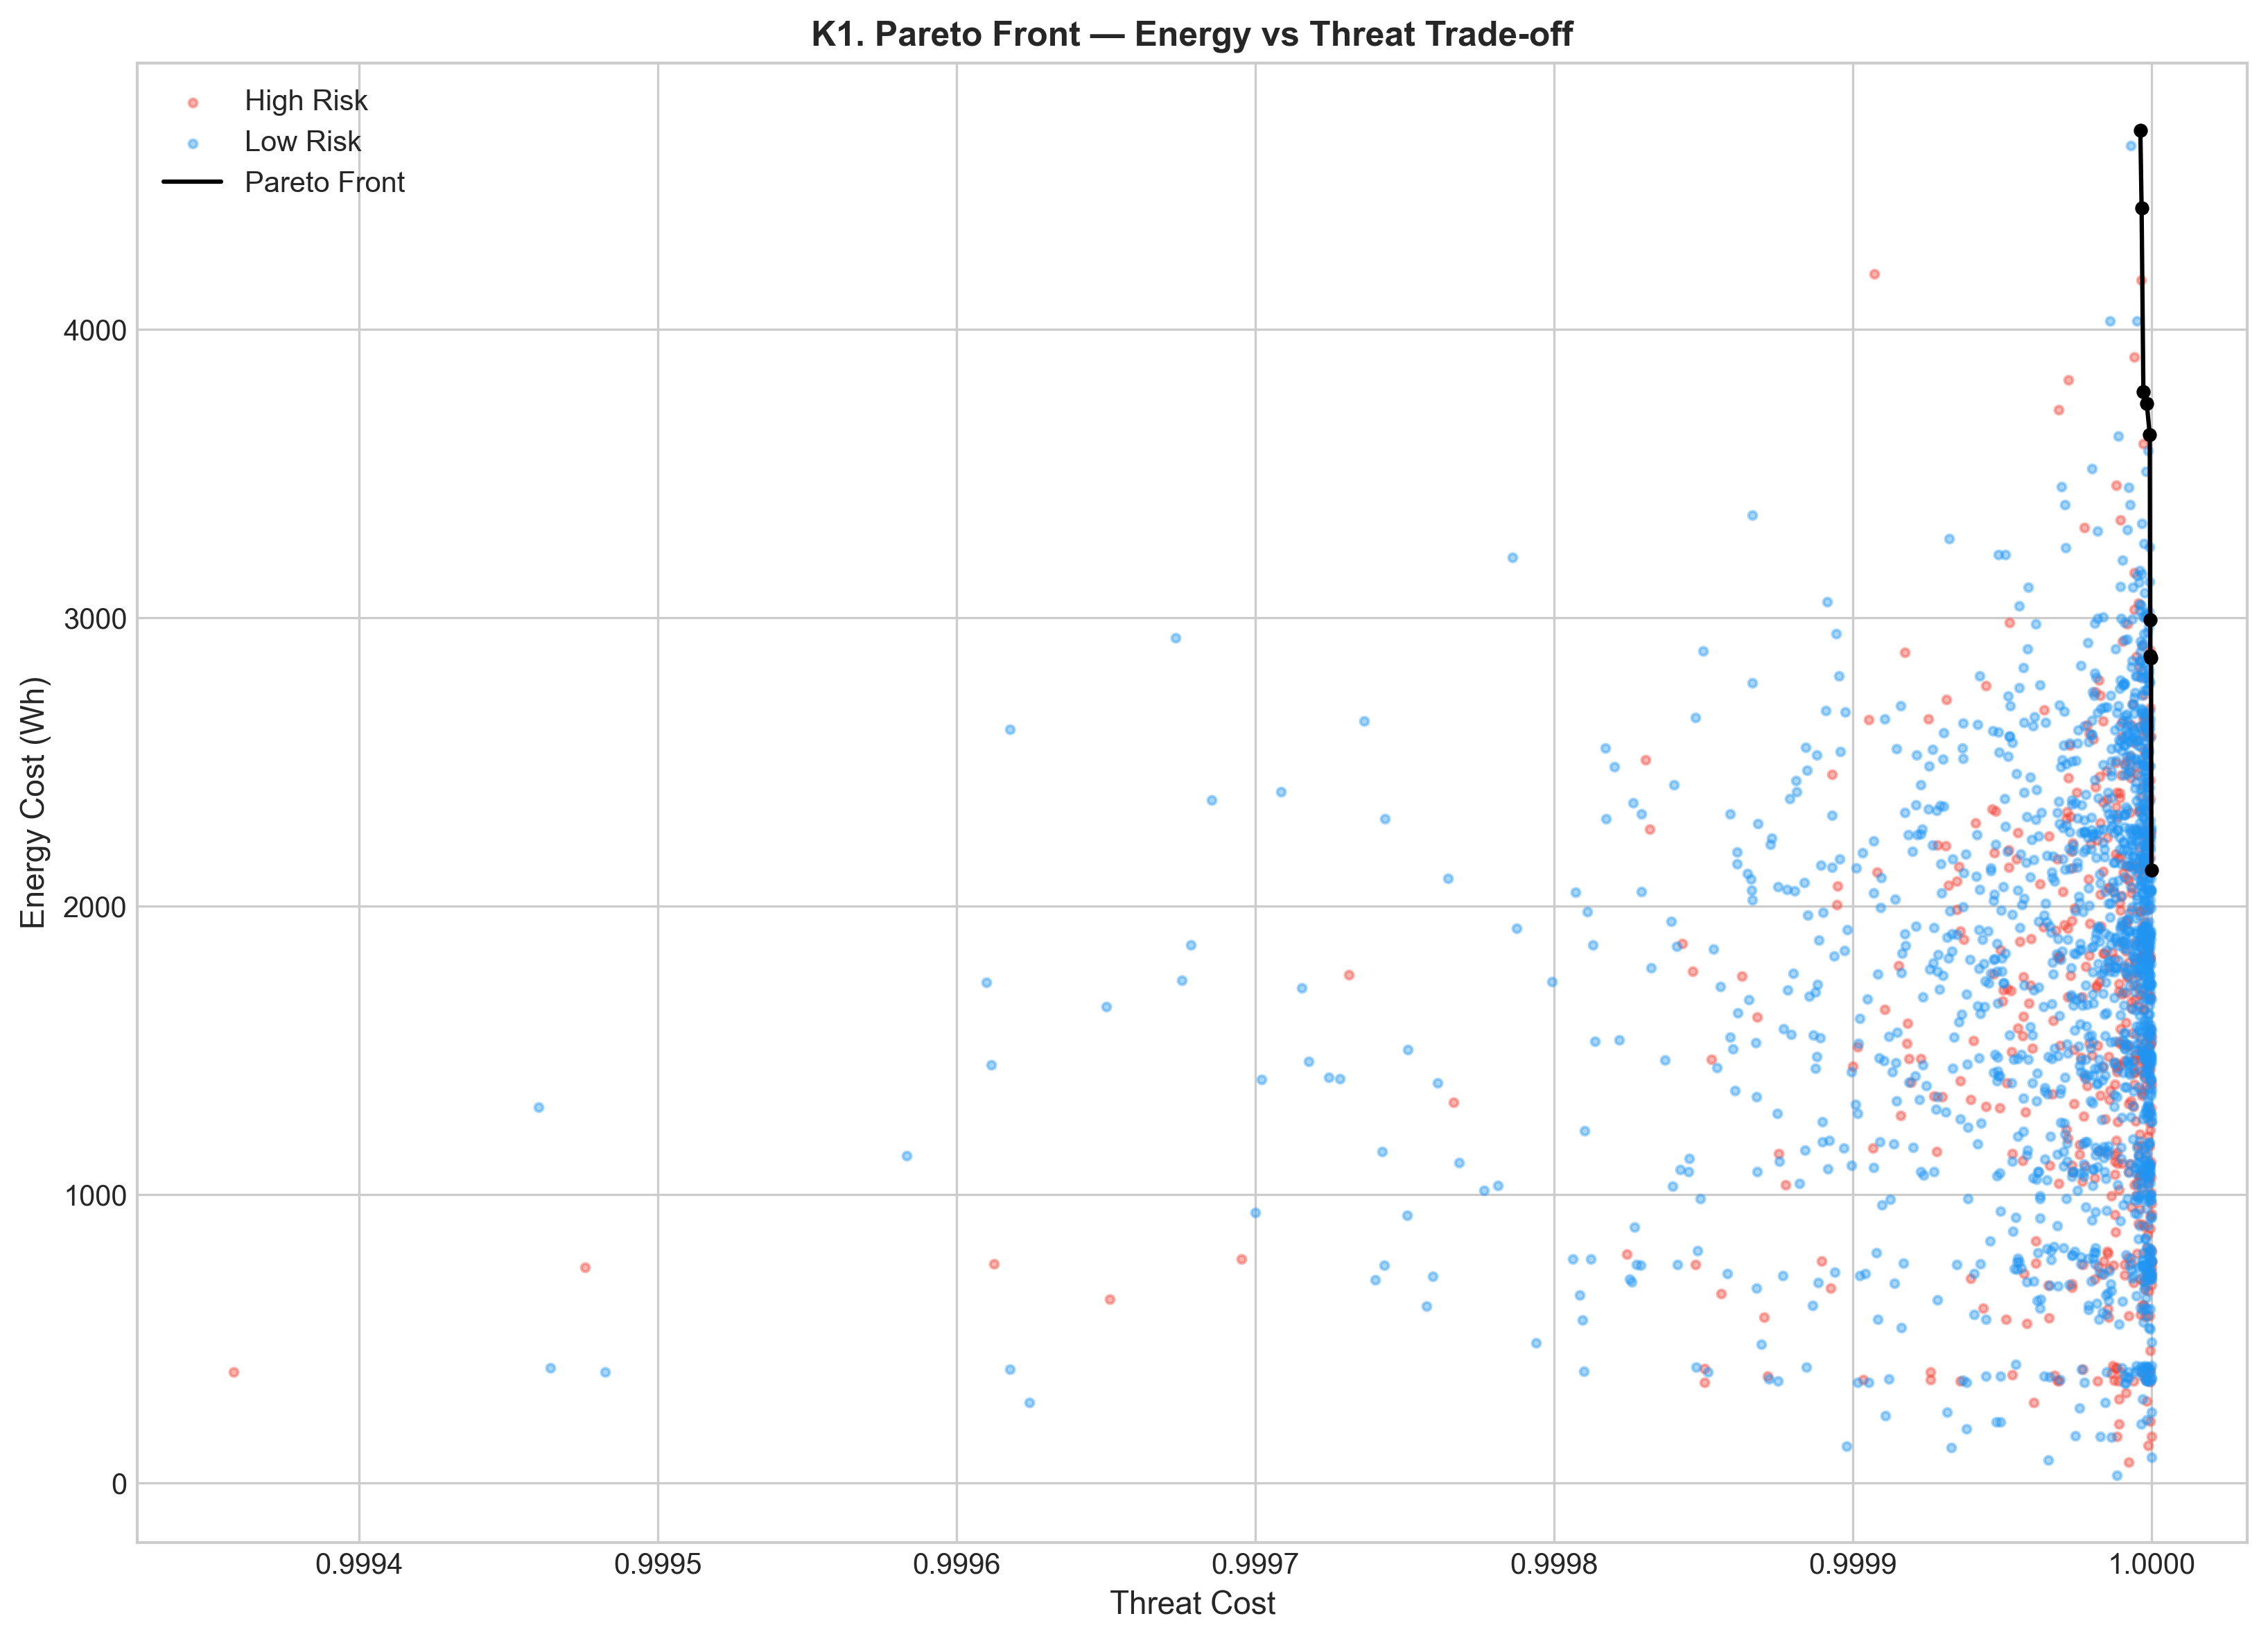
\includegraphics[width=0.72\textwidth]{figures/planning_K1_pareto_front.png}
  \caption{NSGA-III Pareto front: energy vs.\ mission time vs.\ maximum
    threat cost for Delhi. The 3D front illustrates the non-dominated
    solution structure that makes OC-3 (Pareto ranking) a non-trivial task.}
  \label{fig:pareto}
\end{figure}

\begin{figure}[h]
  \centering
  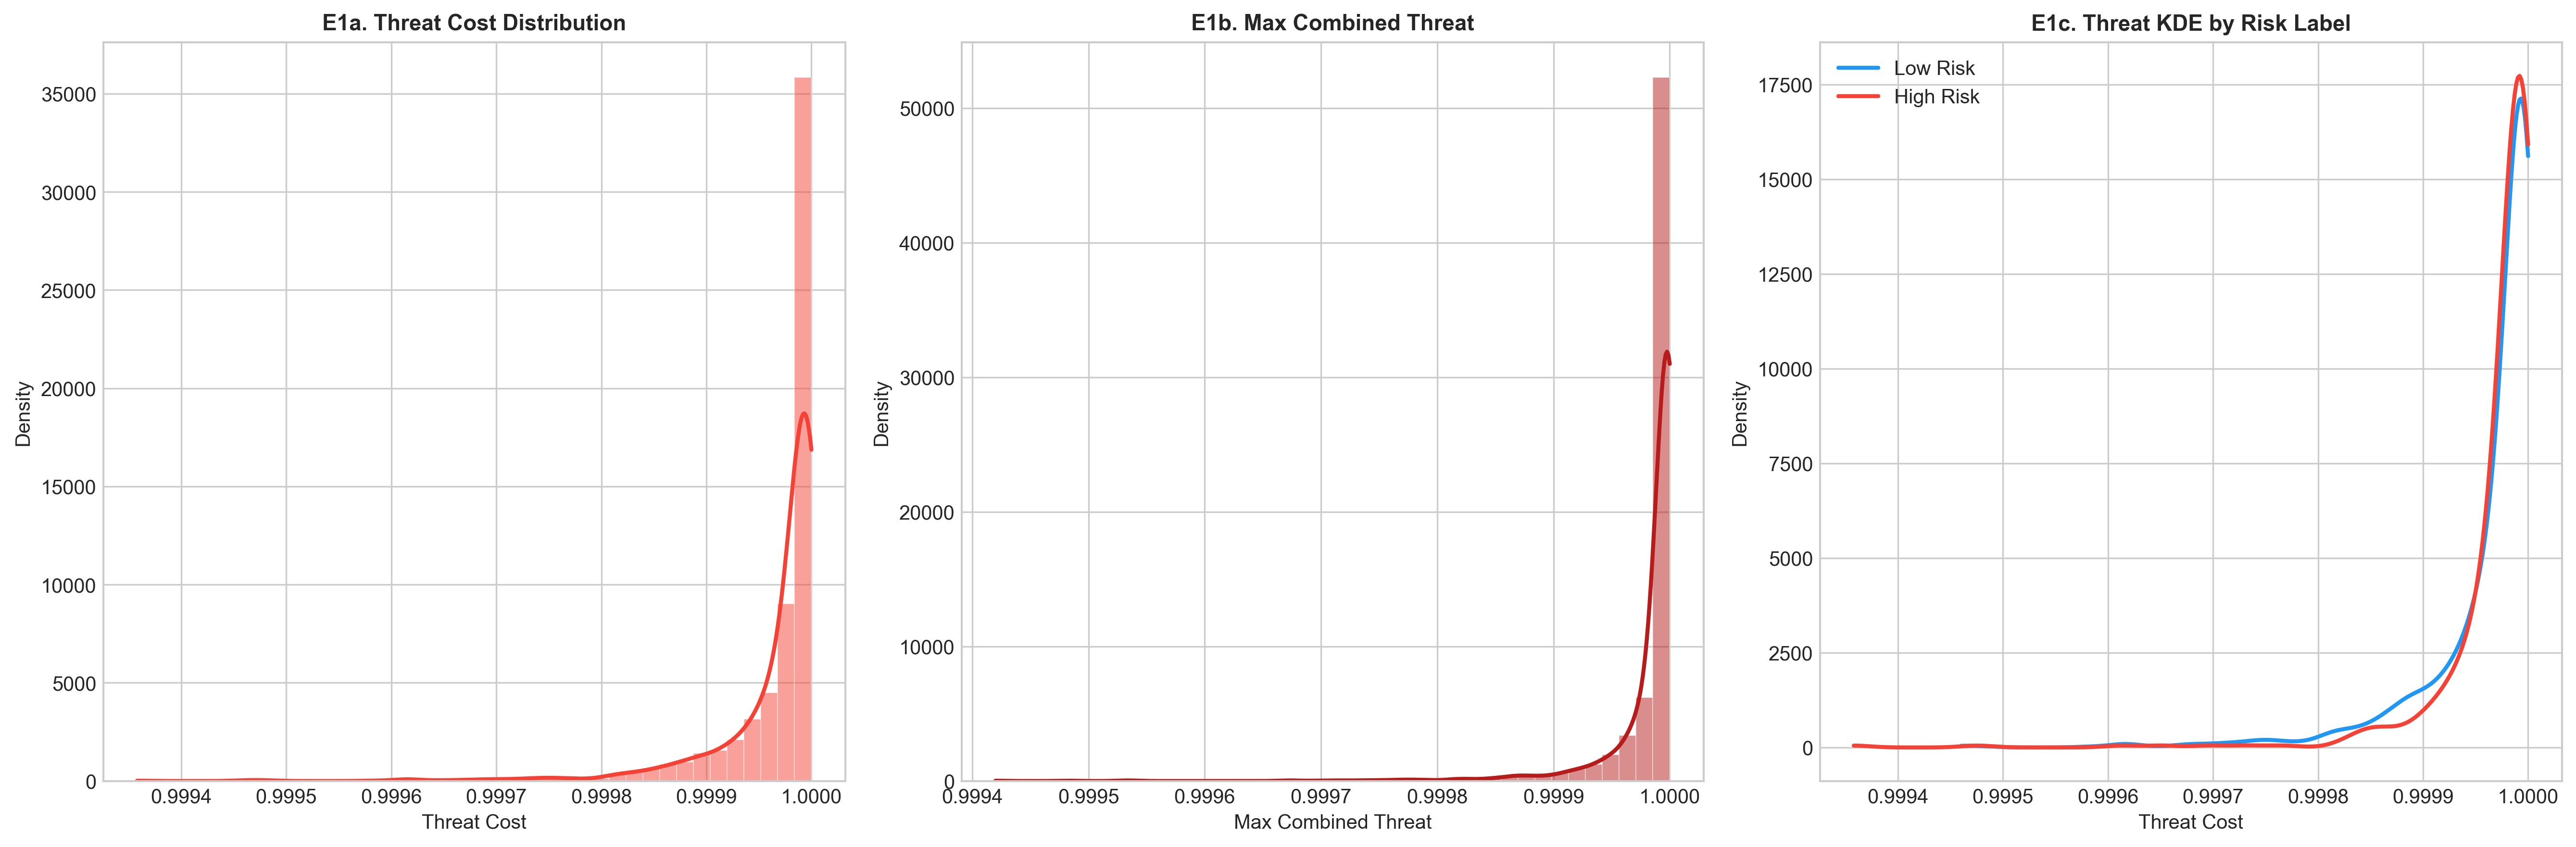
\includegraphics[width=0.72\textwidth]{figures/planning_E1_threat_distributions.png}
  \caption{Distribution of \texttt{max\_combined\_threat} per region.
    The bimodal structure in balanced regions (Delhi, Mumbai, Bangalore)
    motivates the 0.35 threshold; near-degenerate regions (Arunachal, Ladakh)
    produce strongly left-skewed distributions.}
  \label{fig:threat_dist}
\end{figure}

\subsection*{Vehicle Layer}

\begin{figure}[h]
  \centering
  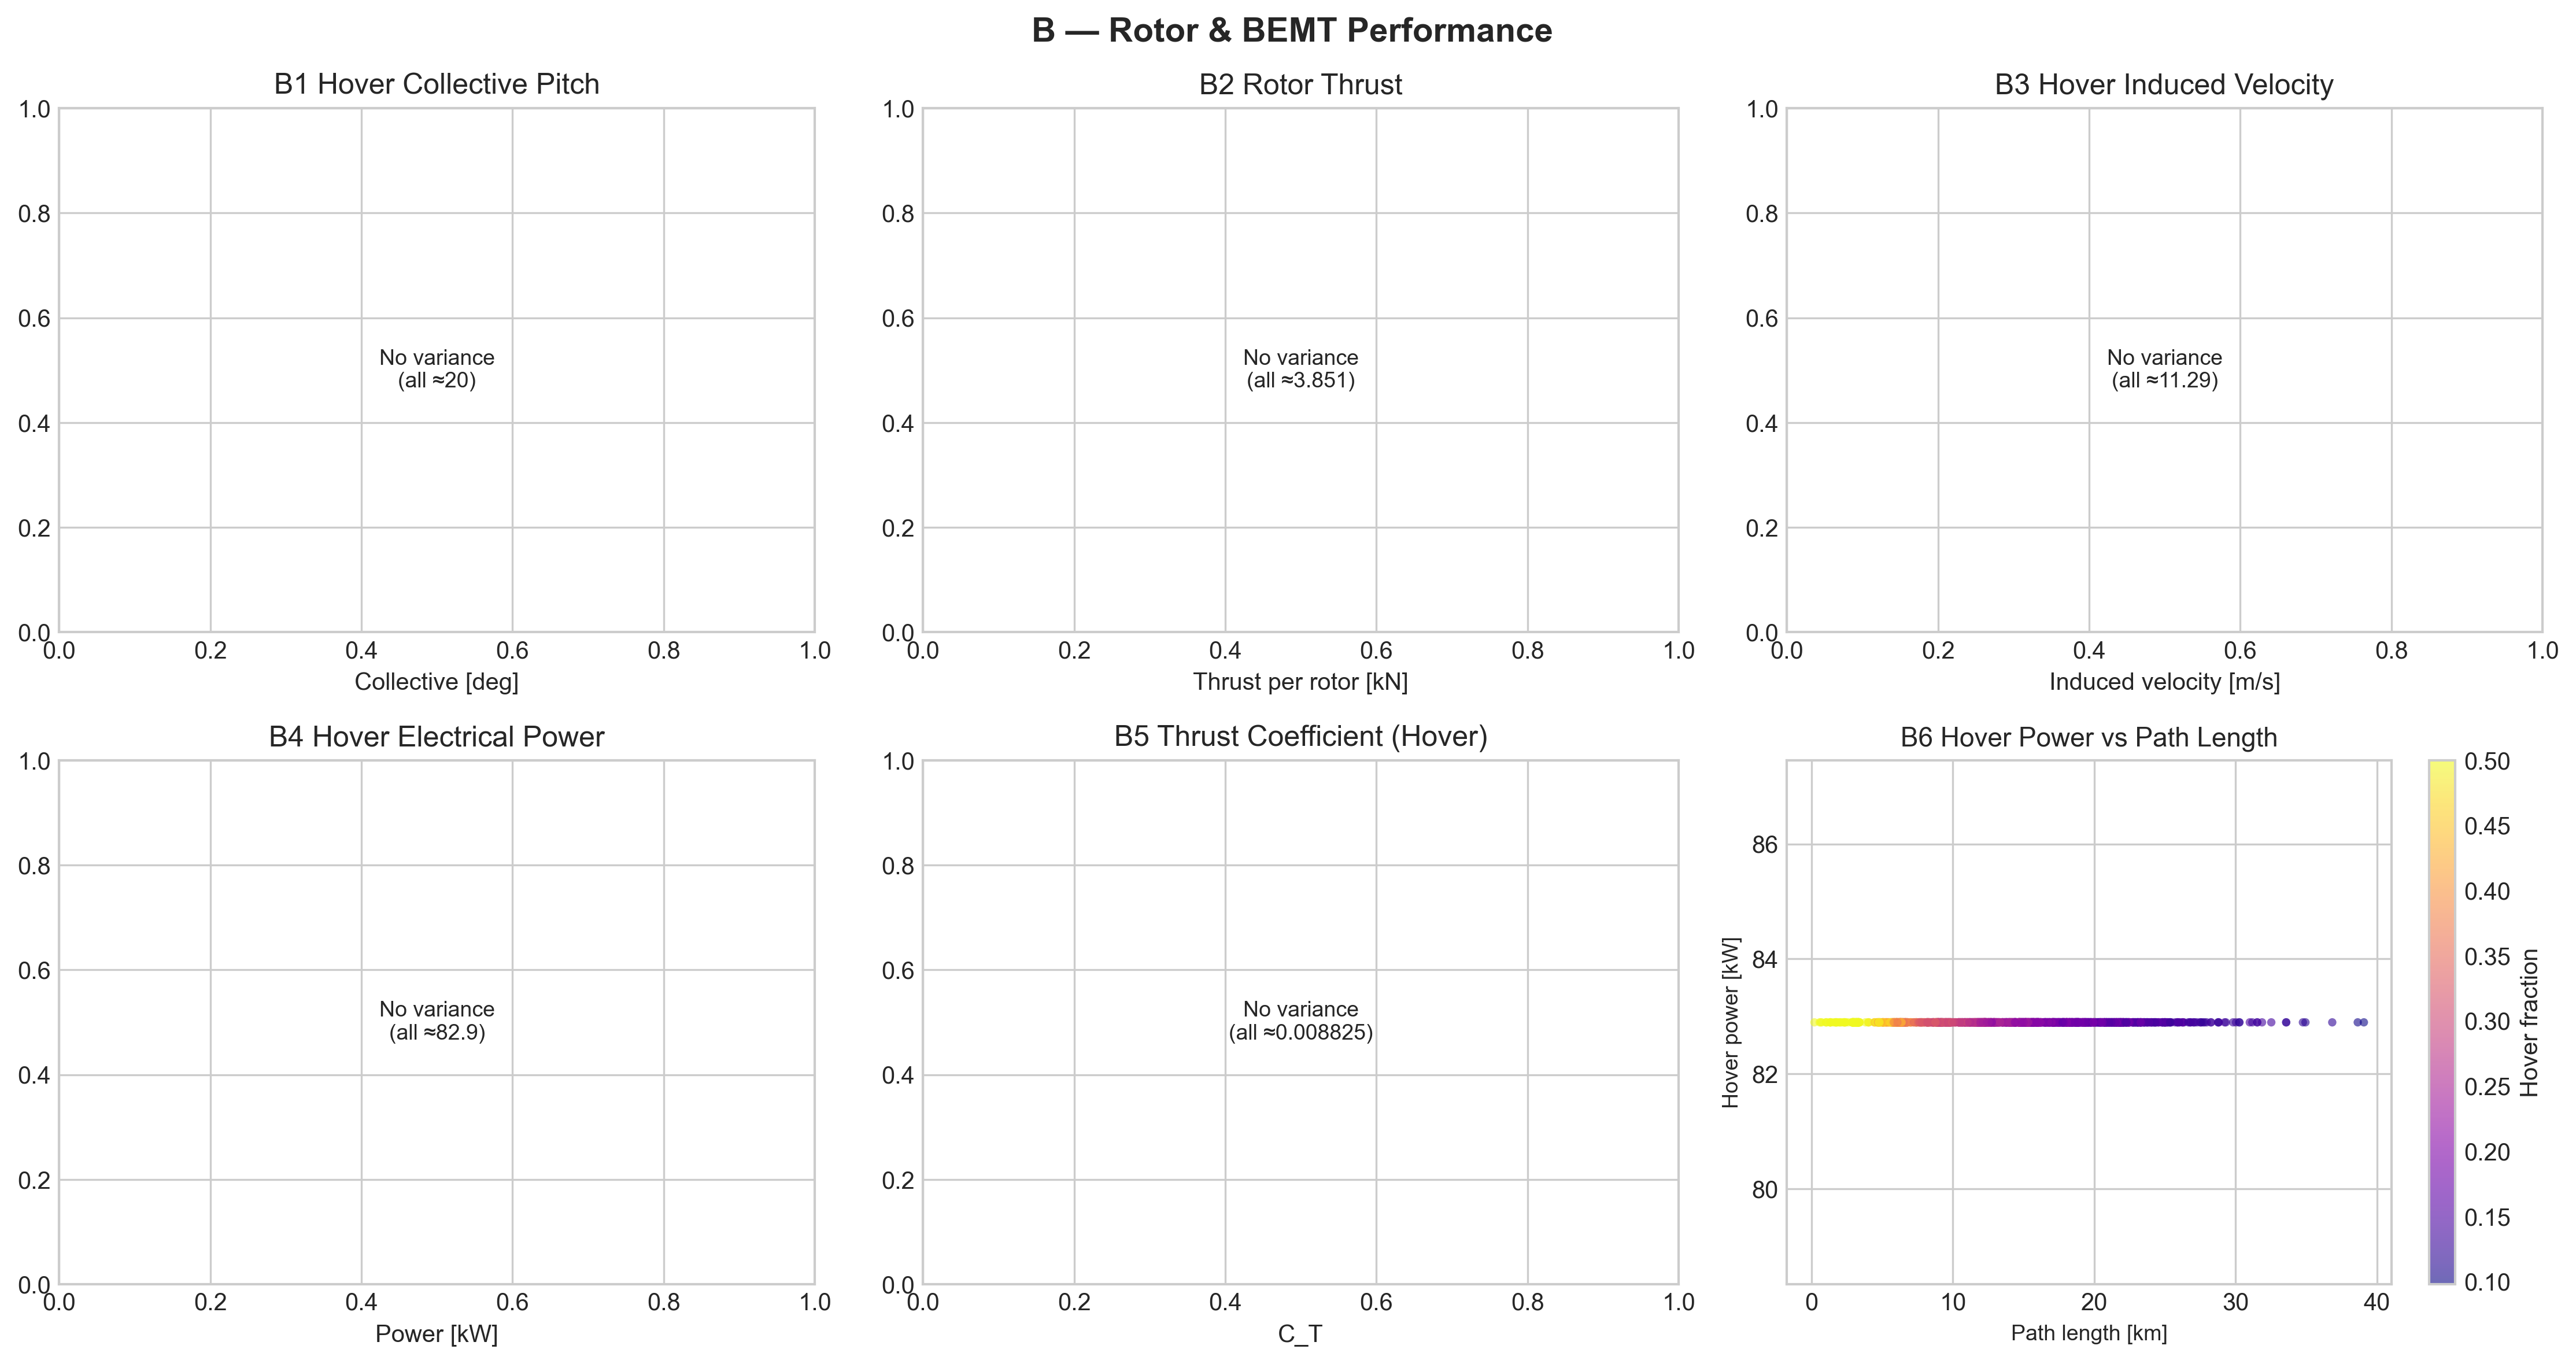
\includegraphics[width=0.72\textwidth]{figures/vehicle_B01_rotor_bemt_performance.png}
  \caption{BEMT rotor performance curves for the 200\,kg-class quad-tiltrotor.
    Figure of merit FM $= C_T^{3/2}/(\sqrt{2}C_P)$ as a function of collective
    pitch angle, used to derive hover efficiency for each mission's
    altitude-adjusted air density.}
  \label{fig:bemt}
\end{figure}

\begin{figure}[h]
  \centering
  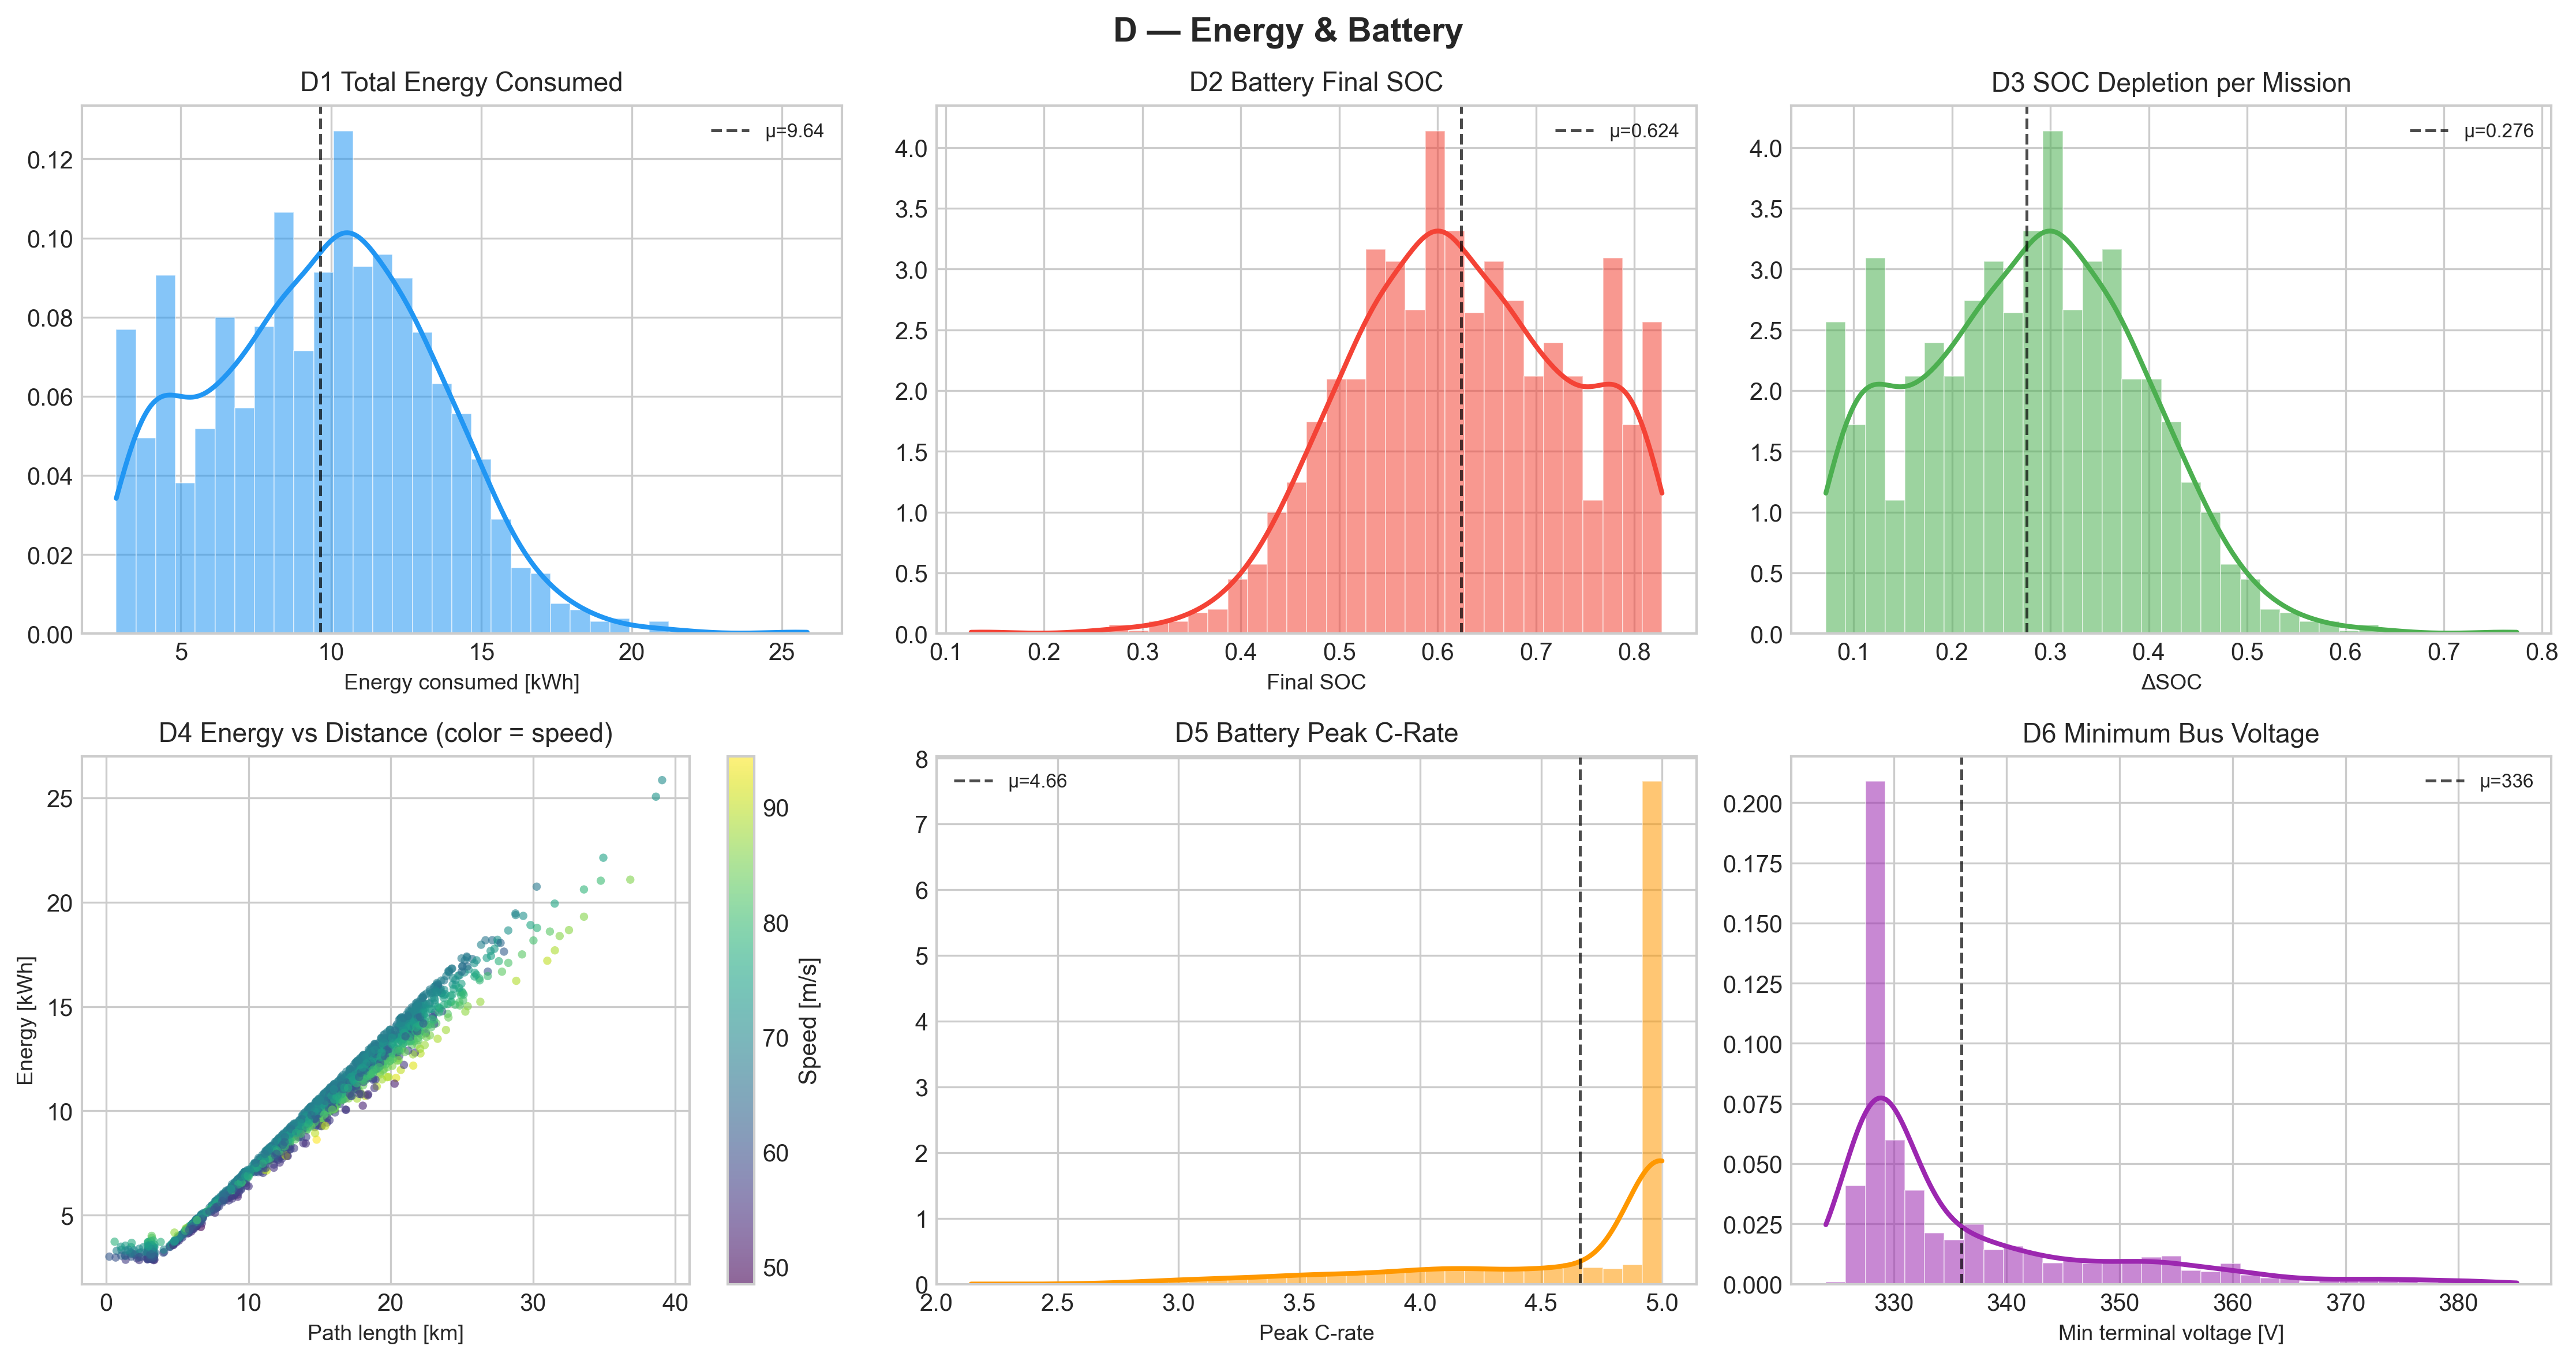
\includegraphics[width=0.72\textwidth]{figures/vehicle_D01_energy_battery.png}
  \caption{Vehicle-layer energy consumption and battery SOC distributions
    (Delhi, $n = 10{,}000$). Log-normal energy distribution motivates
    the log-transform applied to the T2 target.}
  \label{fig:energy}
\end{figure}

\begin{figure}[h]
  \centering
  \begin{subfigure}[b]{0.32\textwidth}
    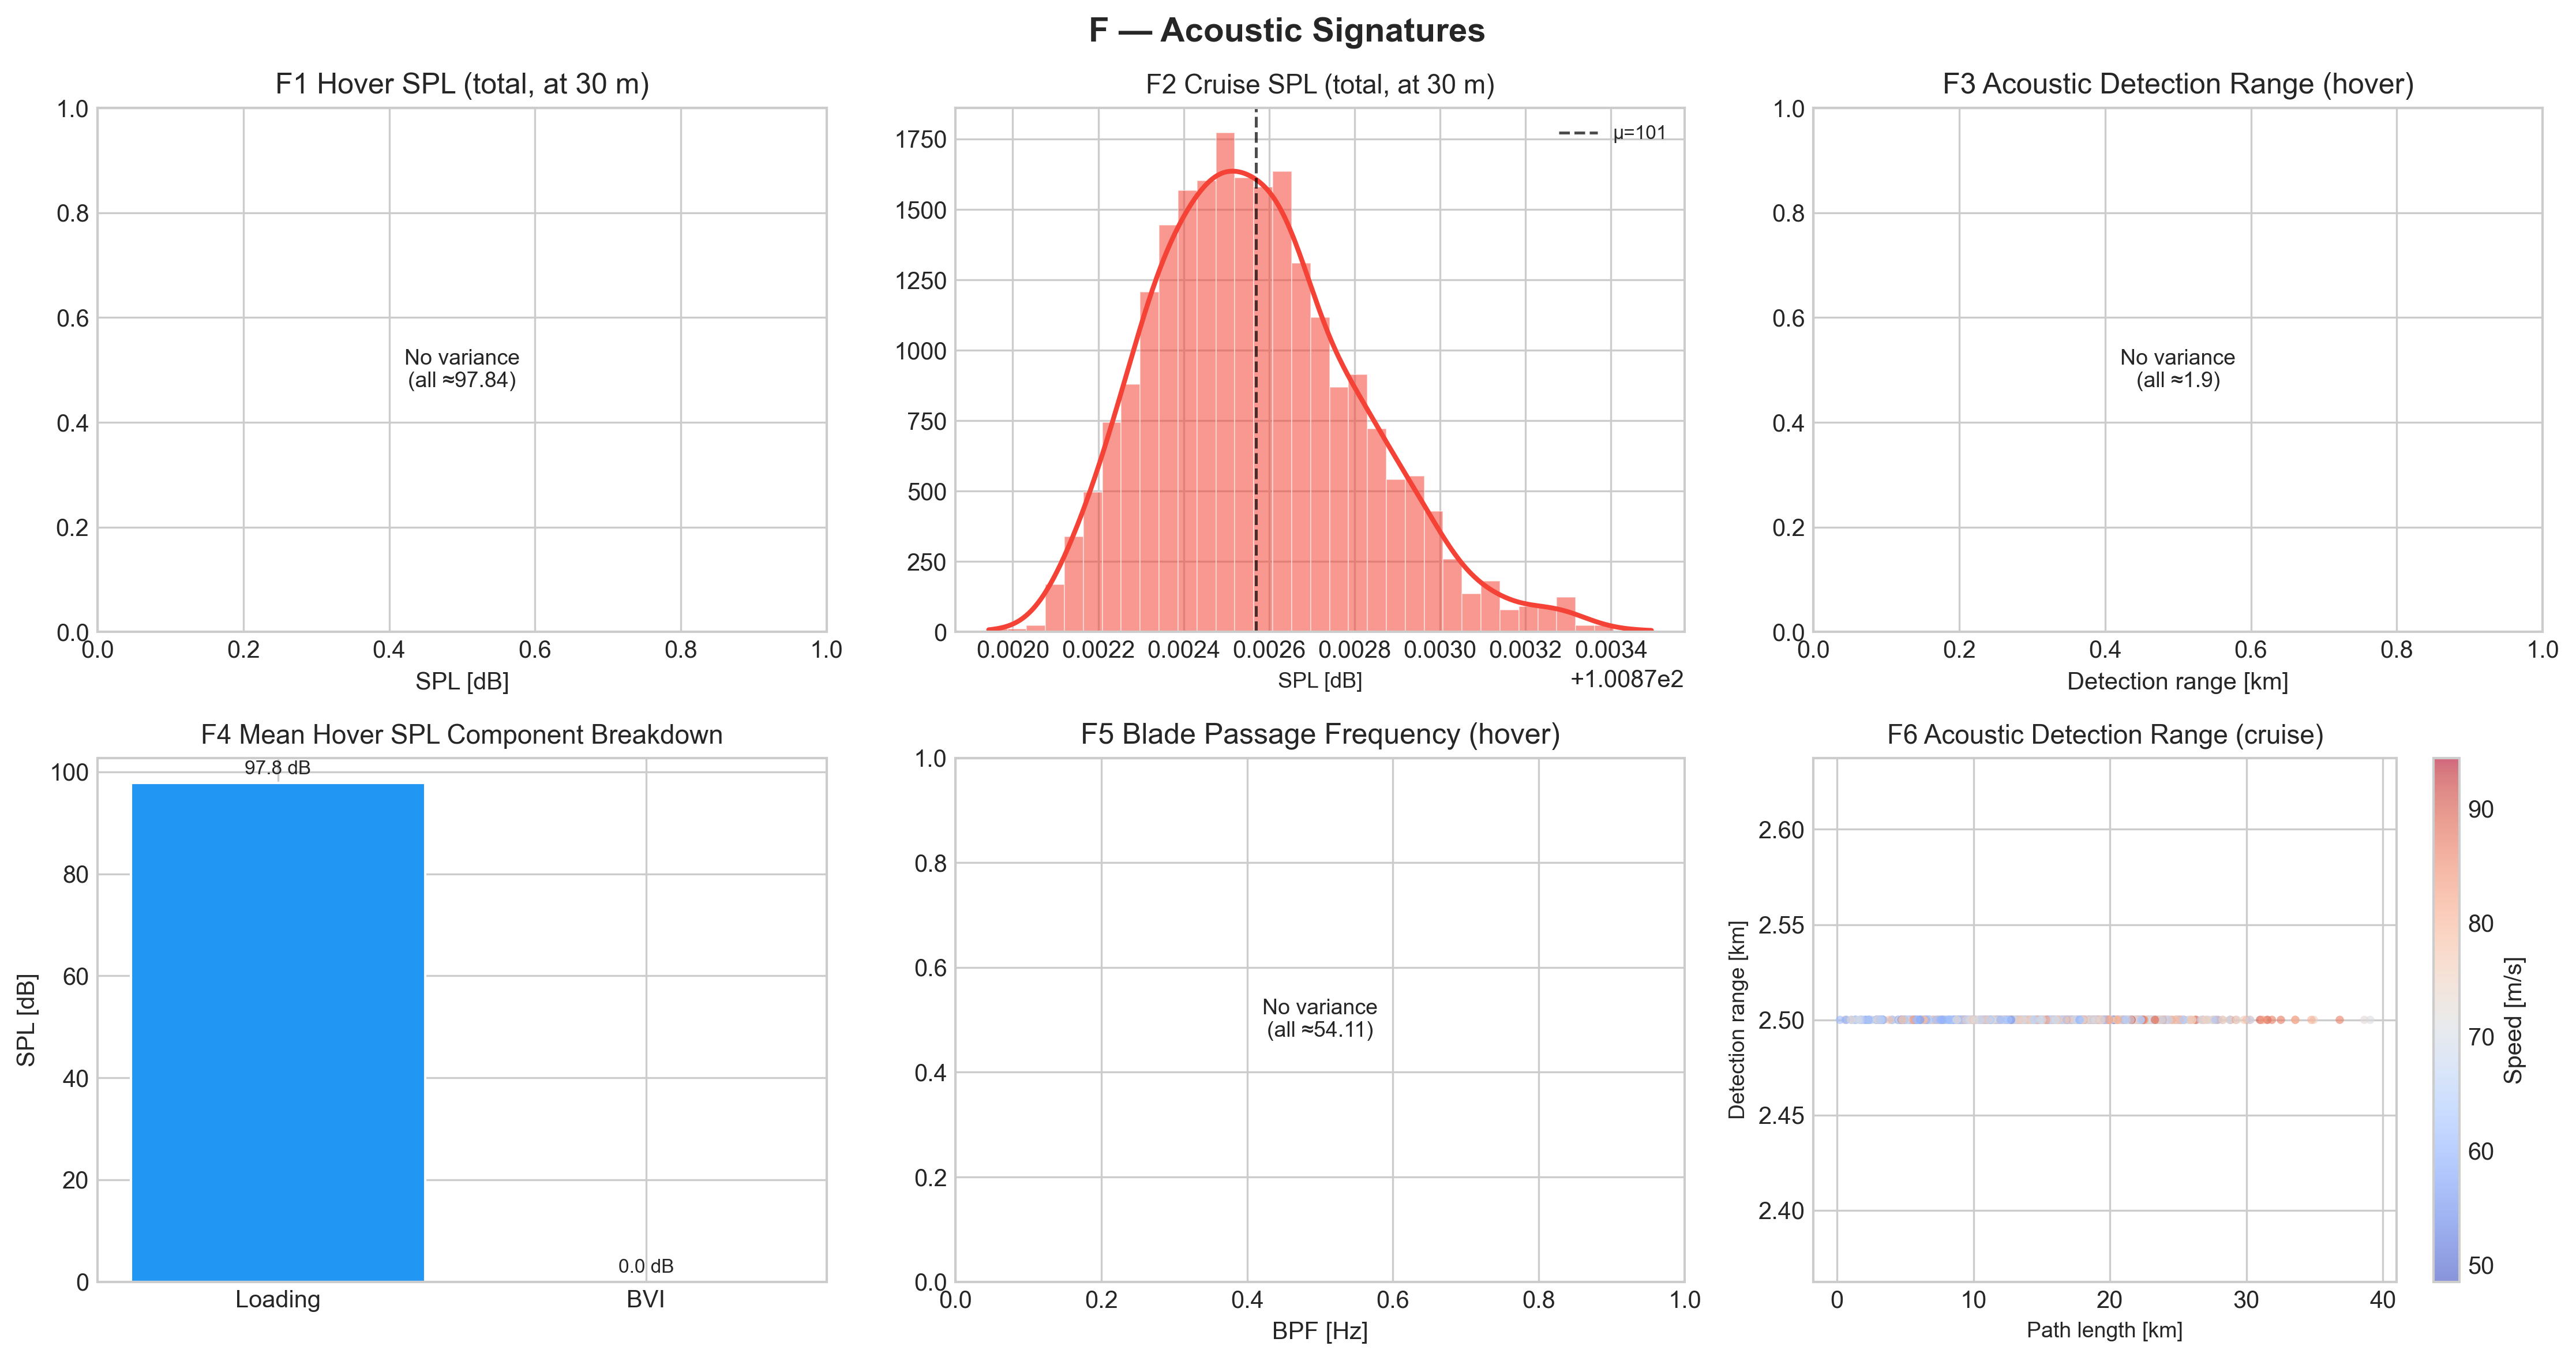
\includegraphics[width=\textwidth]{figures/vehicle_F01_acoustic_signatures.png}
    \caption{Acoustic (FW-H)}
  \end{subfigure}
  \hfill
  \begin{subfigure}[b]{0.32\textwidth}
    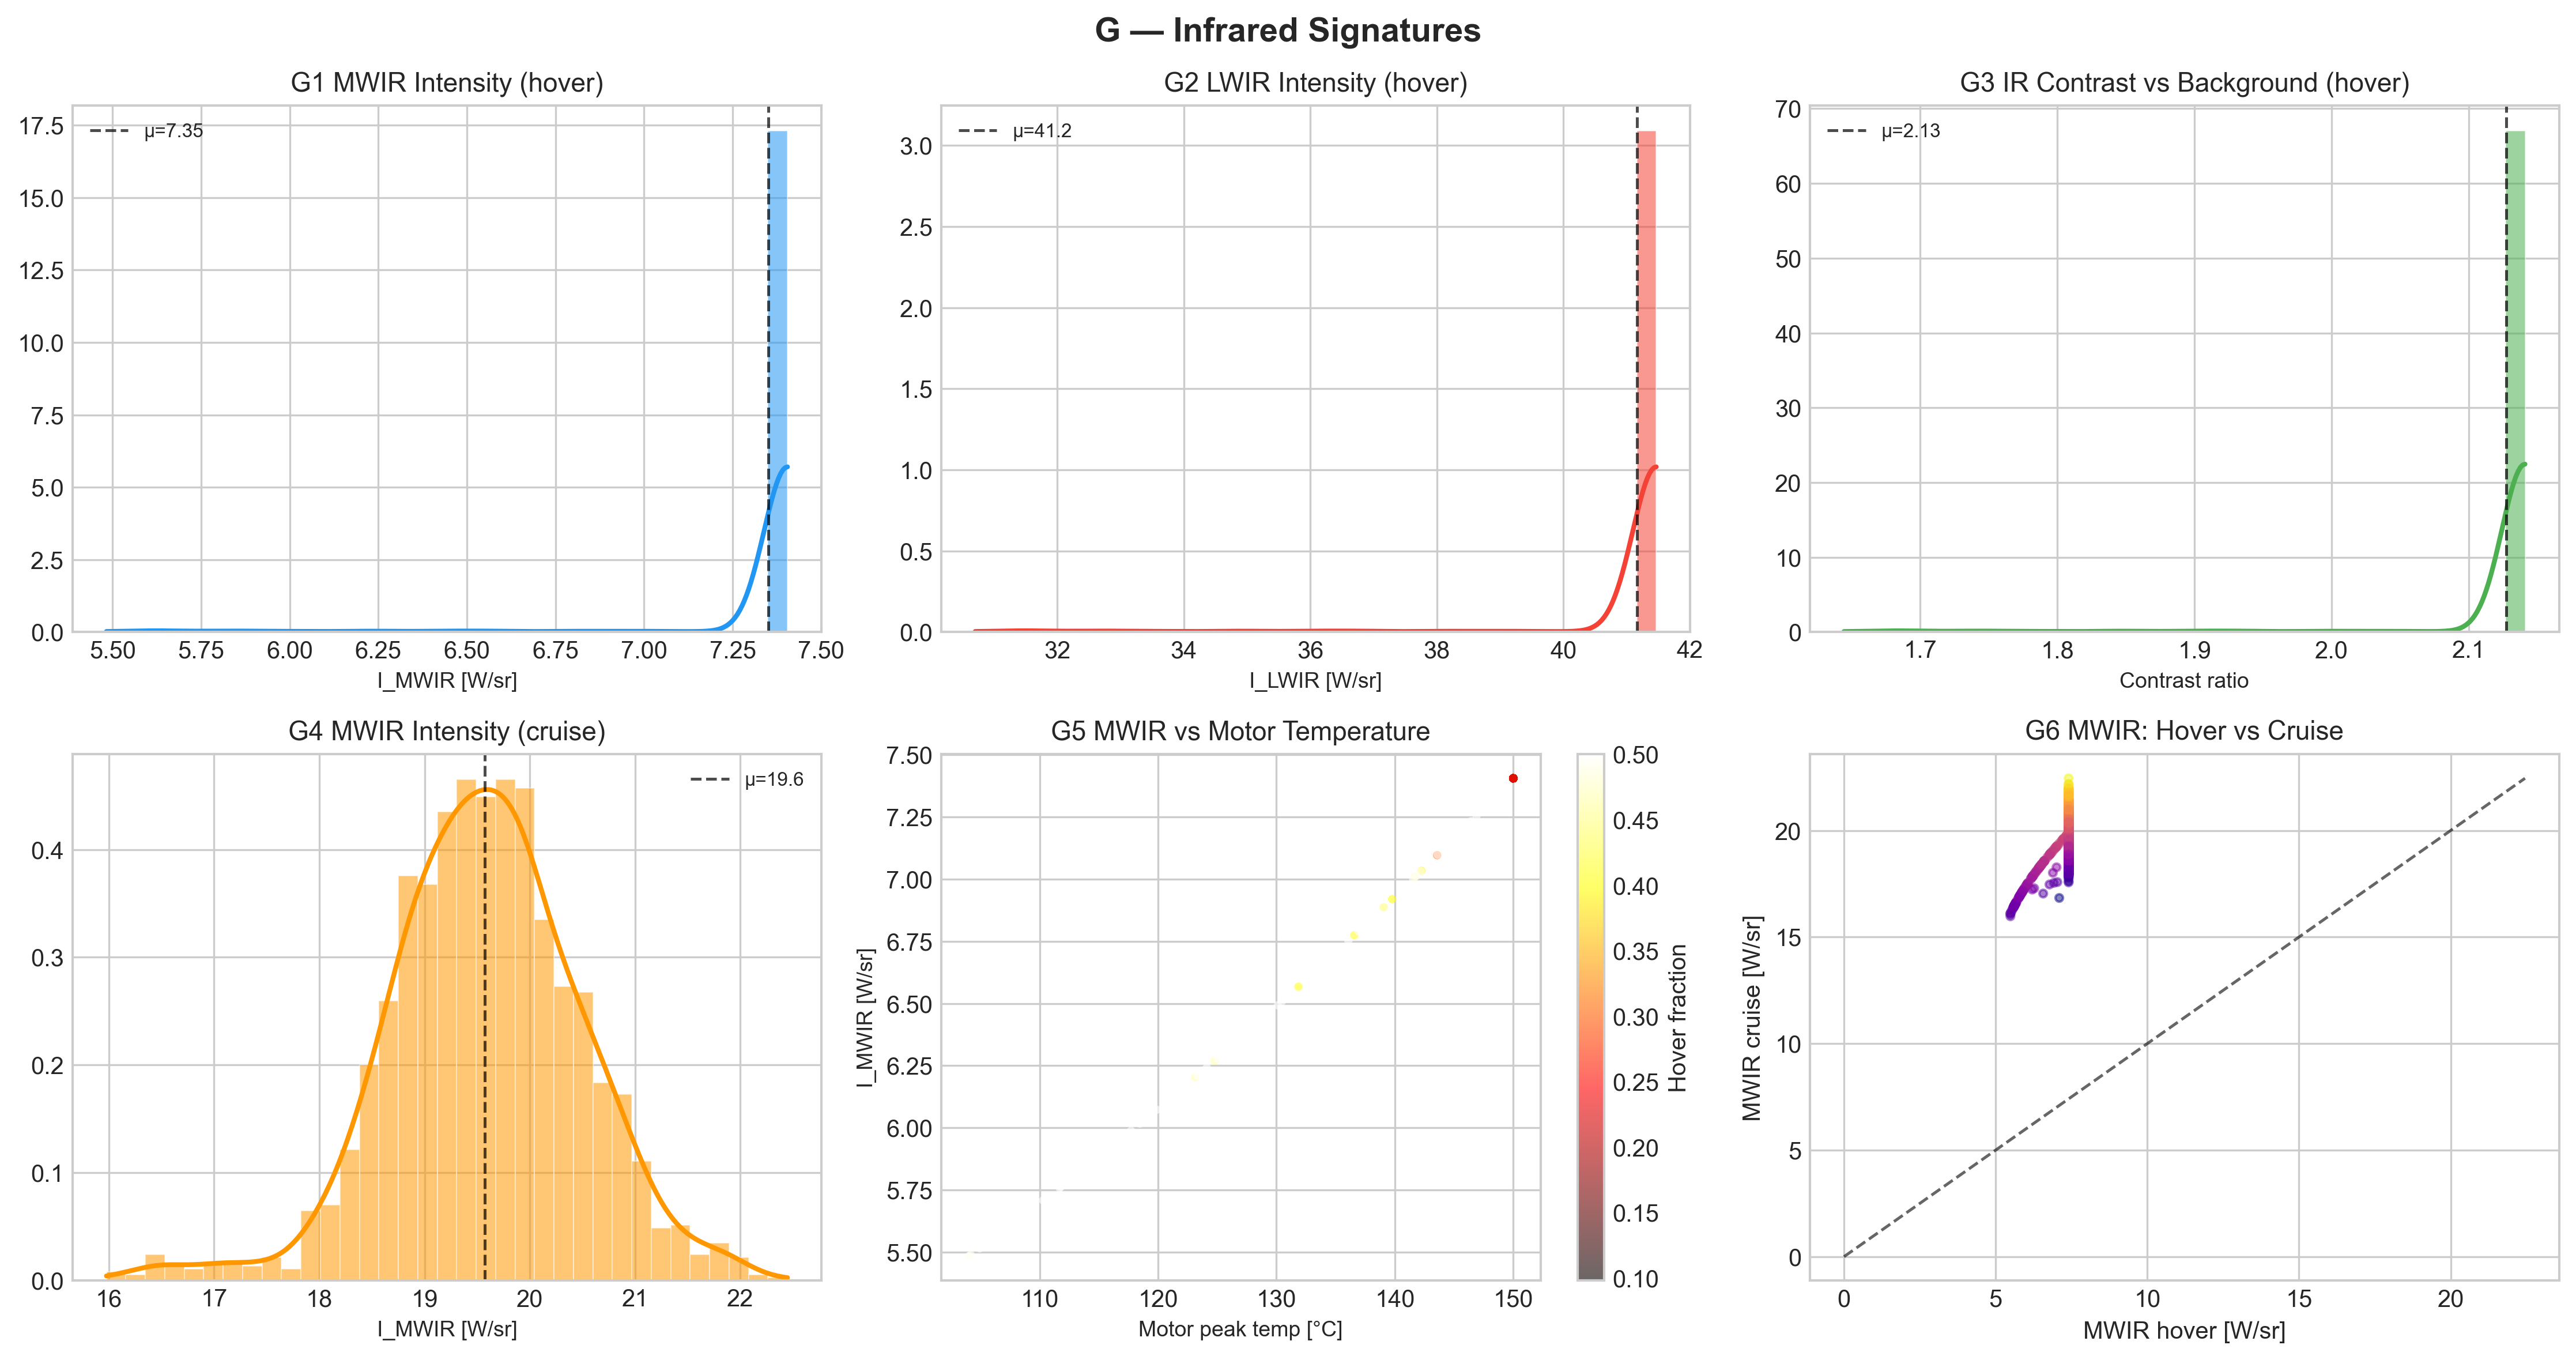
\includegraphics[width=\textwidth]{figures/vehicle_G01_infrared_signatures.png}
    \caption{IR (MWIR/LWIR)}
  \end{subfigure}
  \hfill
  \begin{subfigure}[b]{0.32\textwidth}
    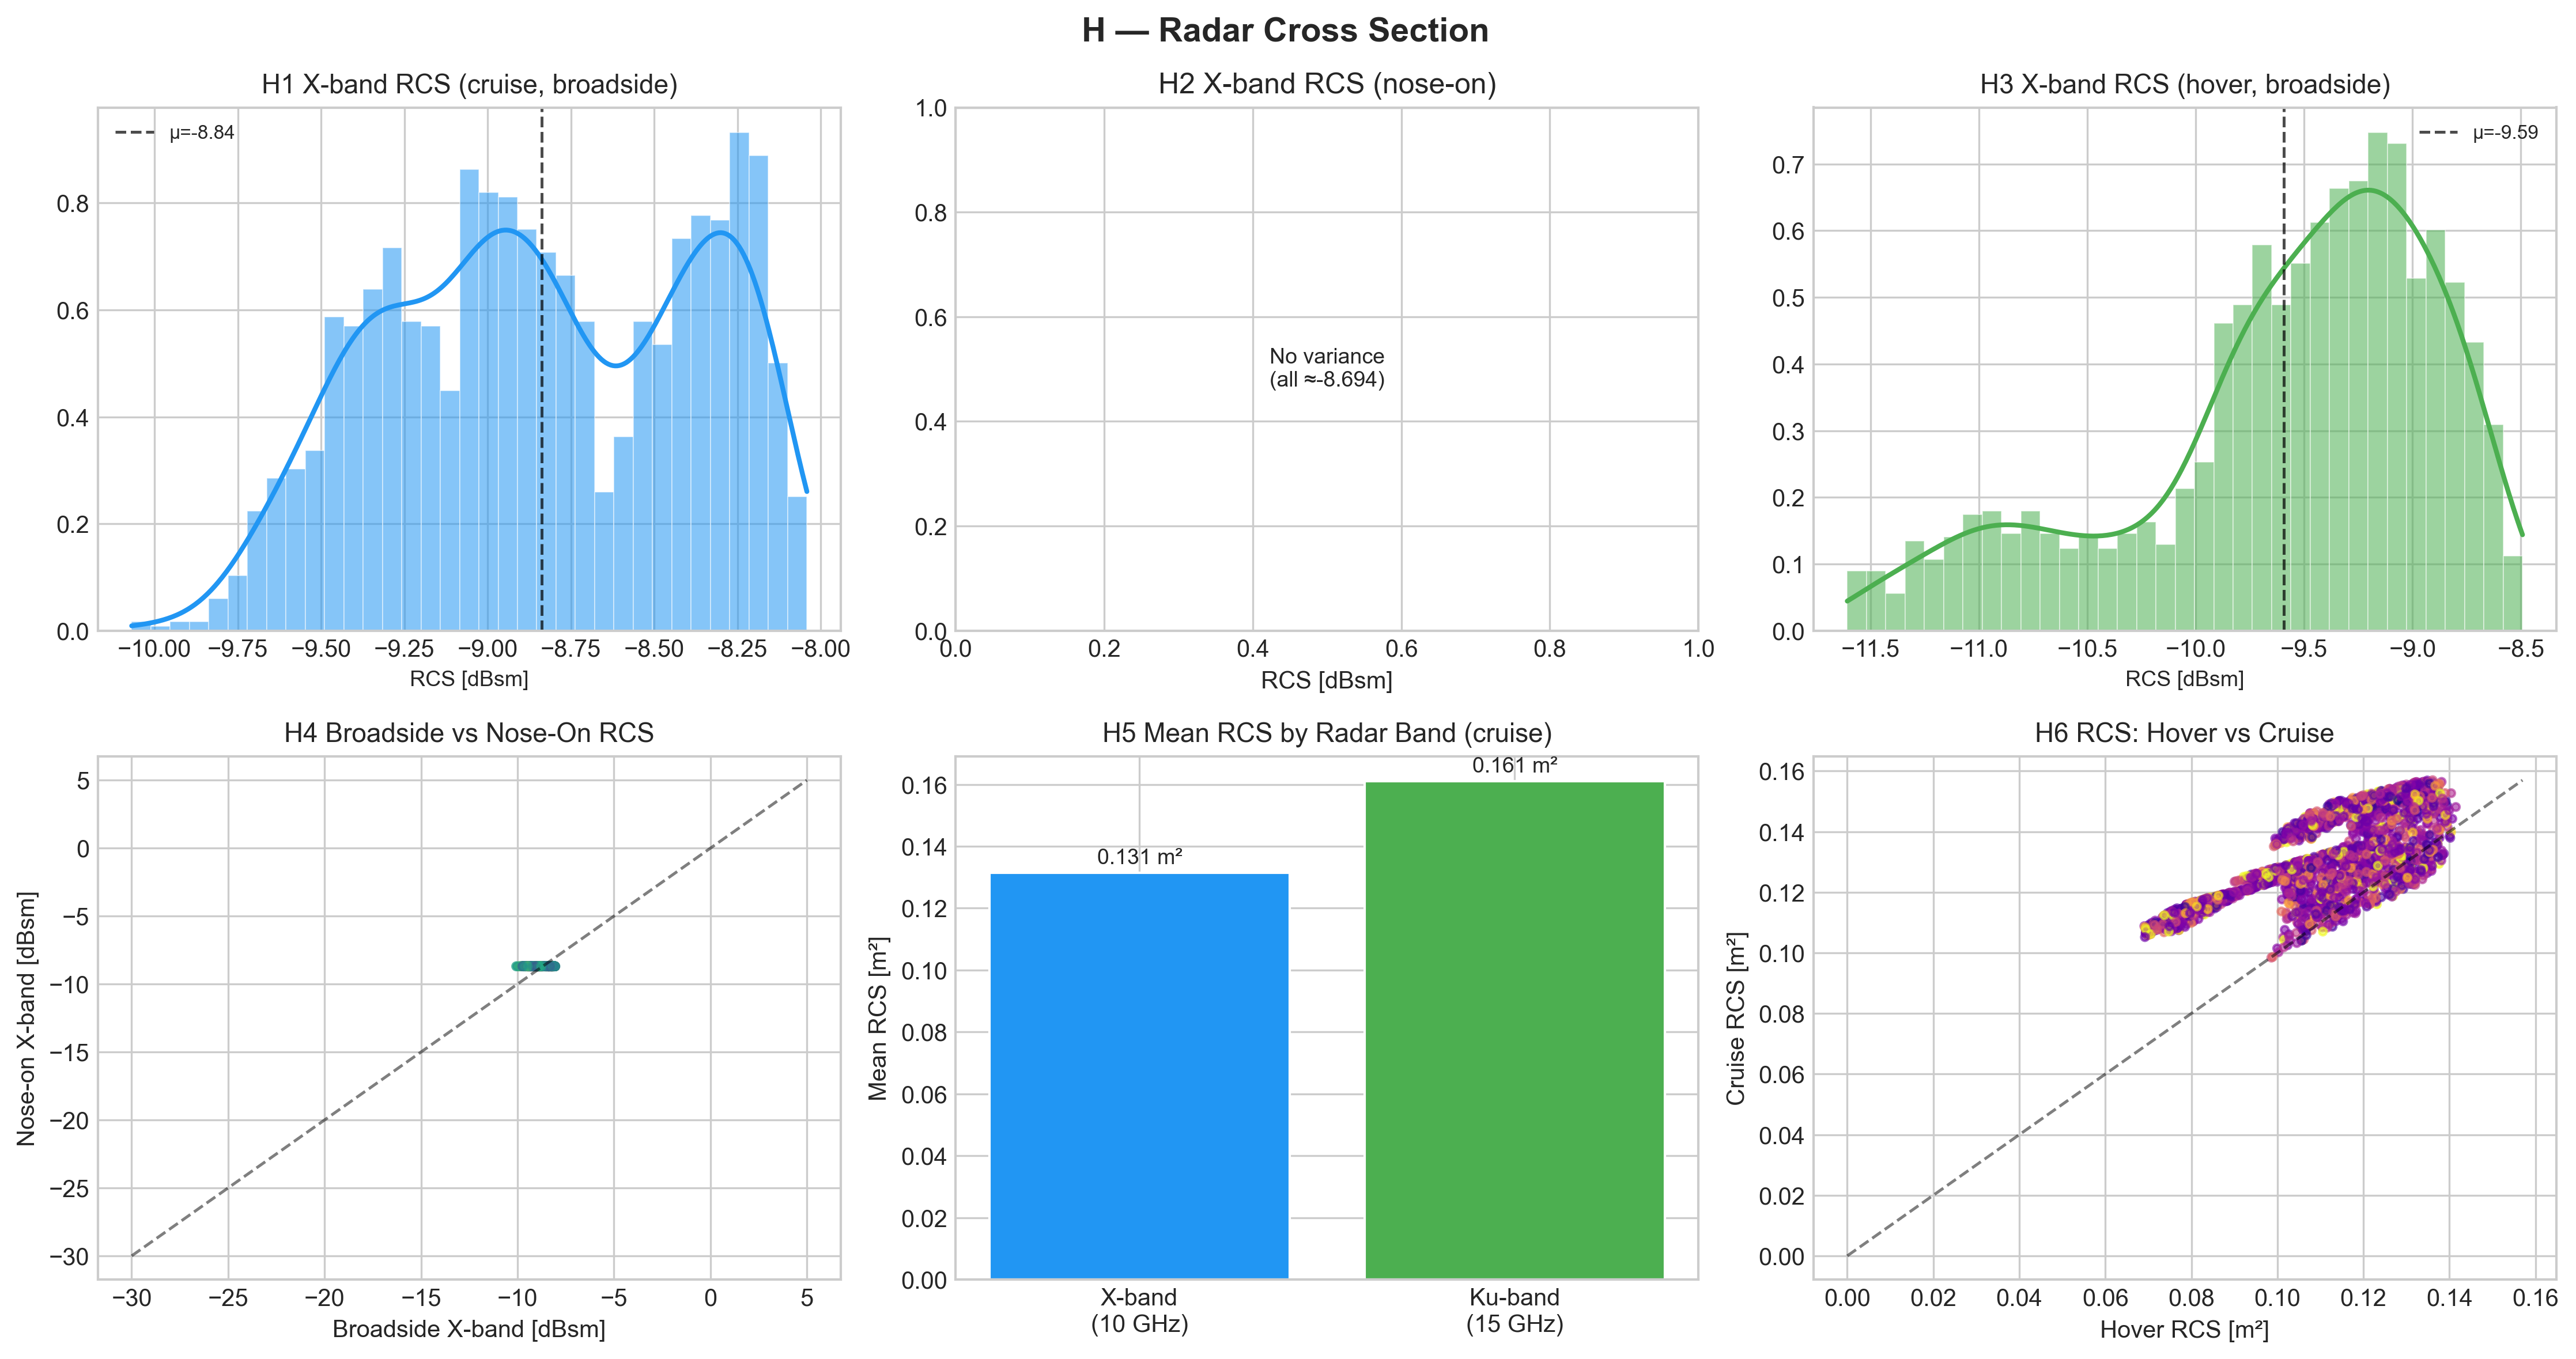
\includegraphics[width=\textwidth]{figures/vehicle_H01_rcs_signatures.png}
    \caption{RCS (X/Ku-band)}
  \end{subfigure}
  \caption{Multi-domain vehicle signature distributions across 10{,}000 Delhi
    missions. Acoustic signatures (left) show log-normal SPL distributions;
    IR signatures (centre) track motor and battery heat; RCS (right) varies
    with aspect angle and rotor position. Together these features underpin OC-3.}
  \label{fig:signatures}
\end{figure}

\begin{figure}[h]
  \centering
  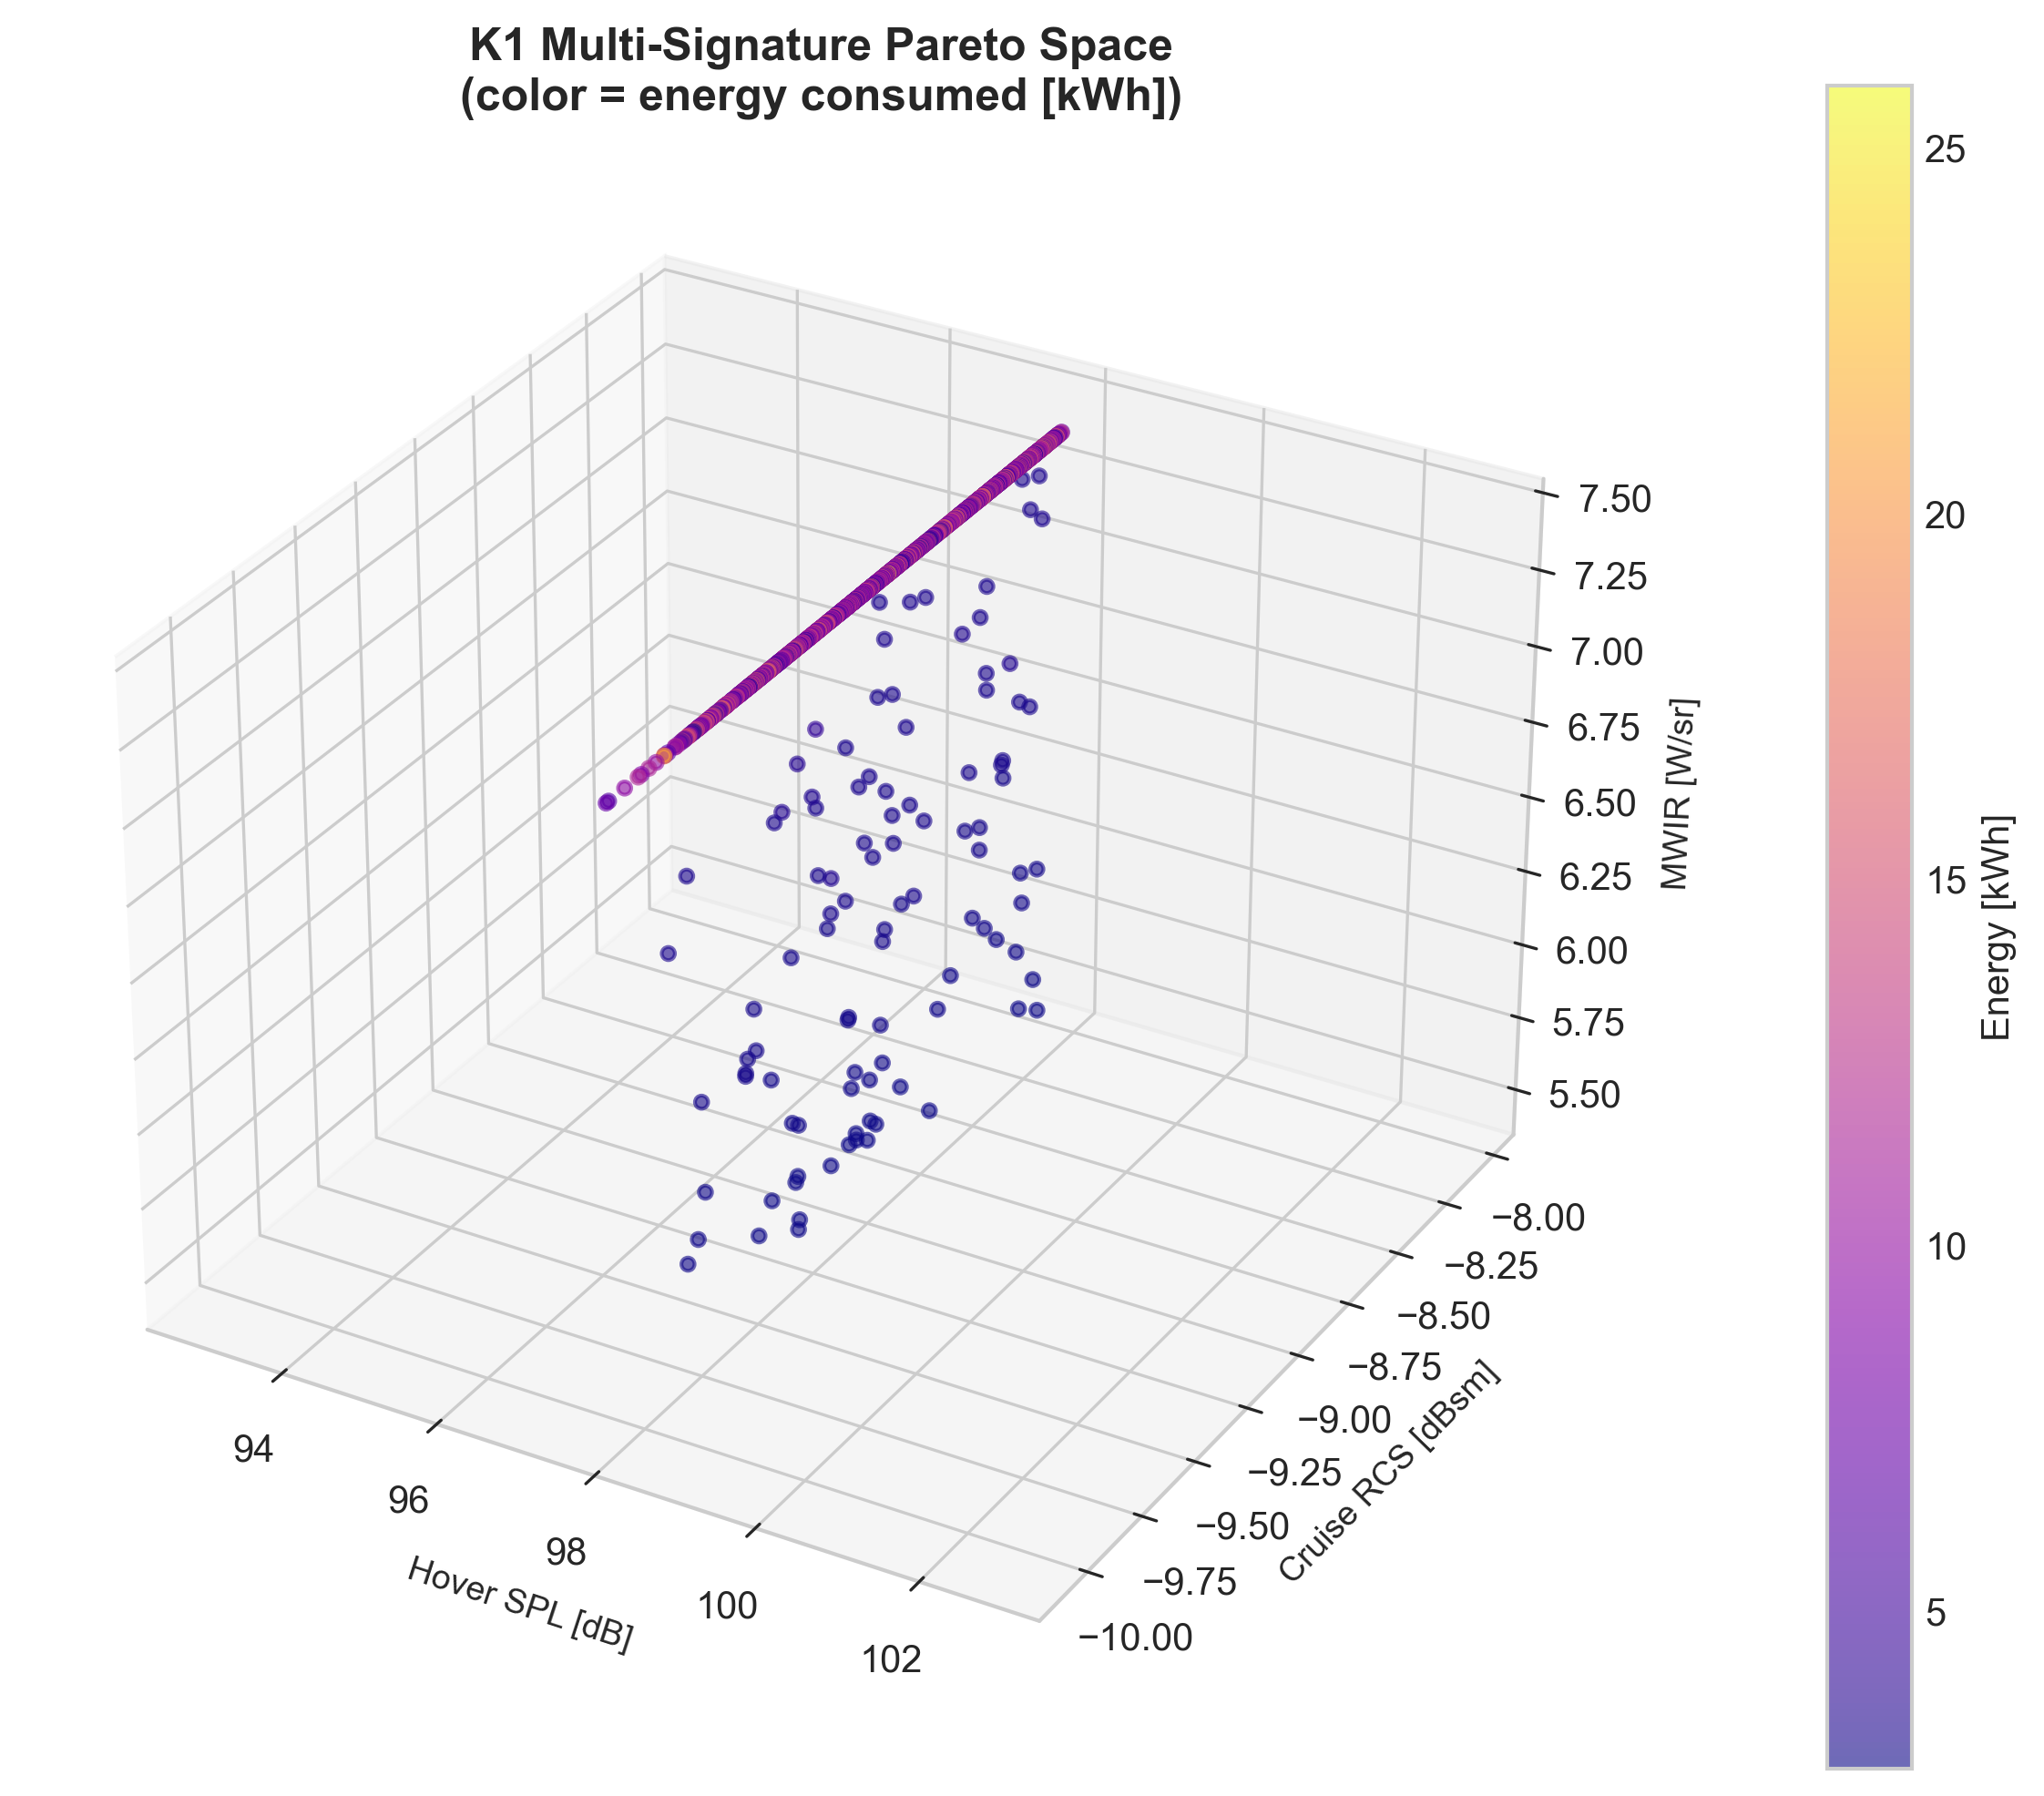
\includegraphics[width=0.72\textwidth]{figures/vehicle_K01_multi_signature_pareto_3d.png}
  \caption{3D Pareto front for multi-signature stealth: acoustic SPL,
    IR irradiance, and RCS trade-offs. Low-signature trajectories
    (dominant solutions) tend to cruise at higher altitude and slower speed.}
  \label{fig:sig_pareto}
\end{figure}

\subsection*{Control Layer}

\begin{figure}[h]
  \centering
  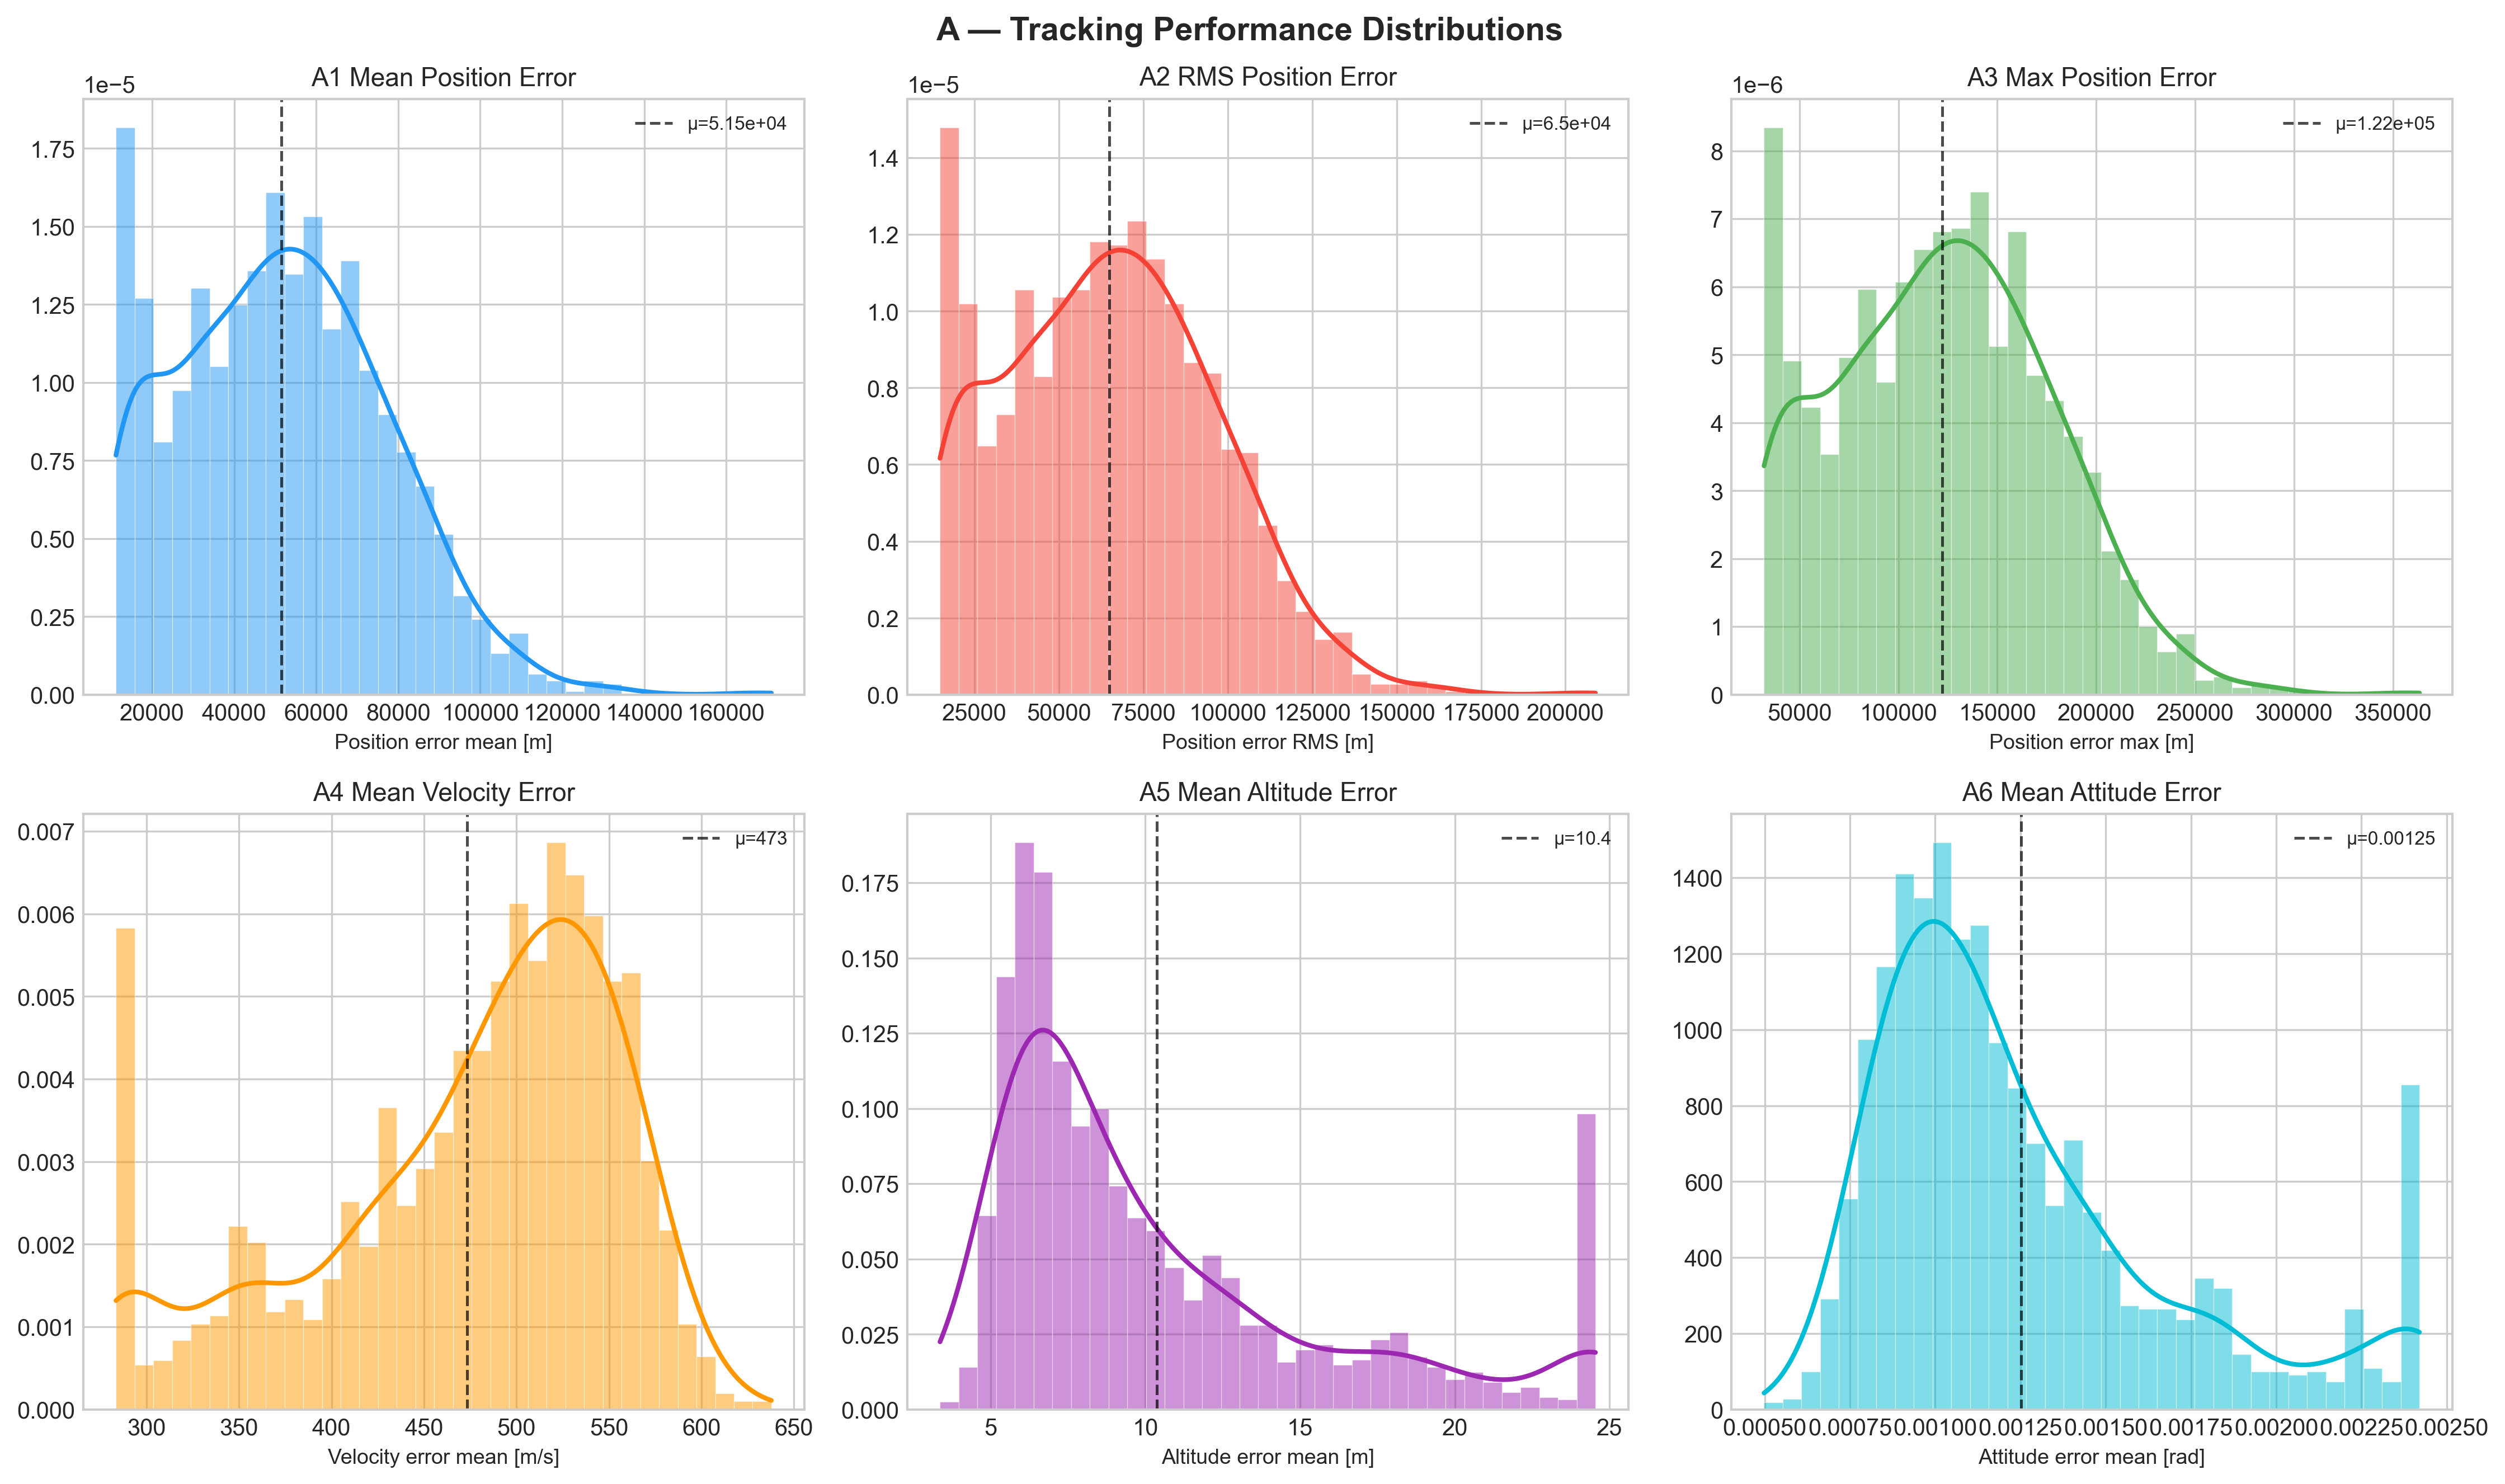
\includegraphics[width=0.72\textwidth]{figures/control_A01_tracking_performance_distributions.png}
  \caption{Control-layer altitude tracking error distributions across mission
    phases. The bimodal structure (low error in cruise, elevated in
    hover--cruise transition) motivates phase-aware T4 models.}
  \label{fig:control}
\end{figure}

\begin{figure}[h]
  \centering
  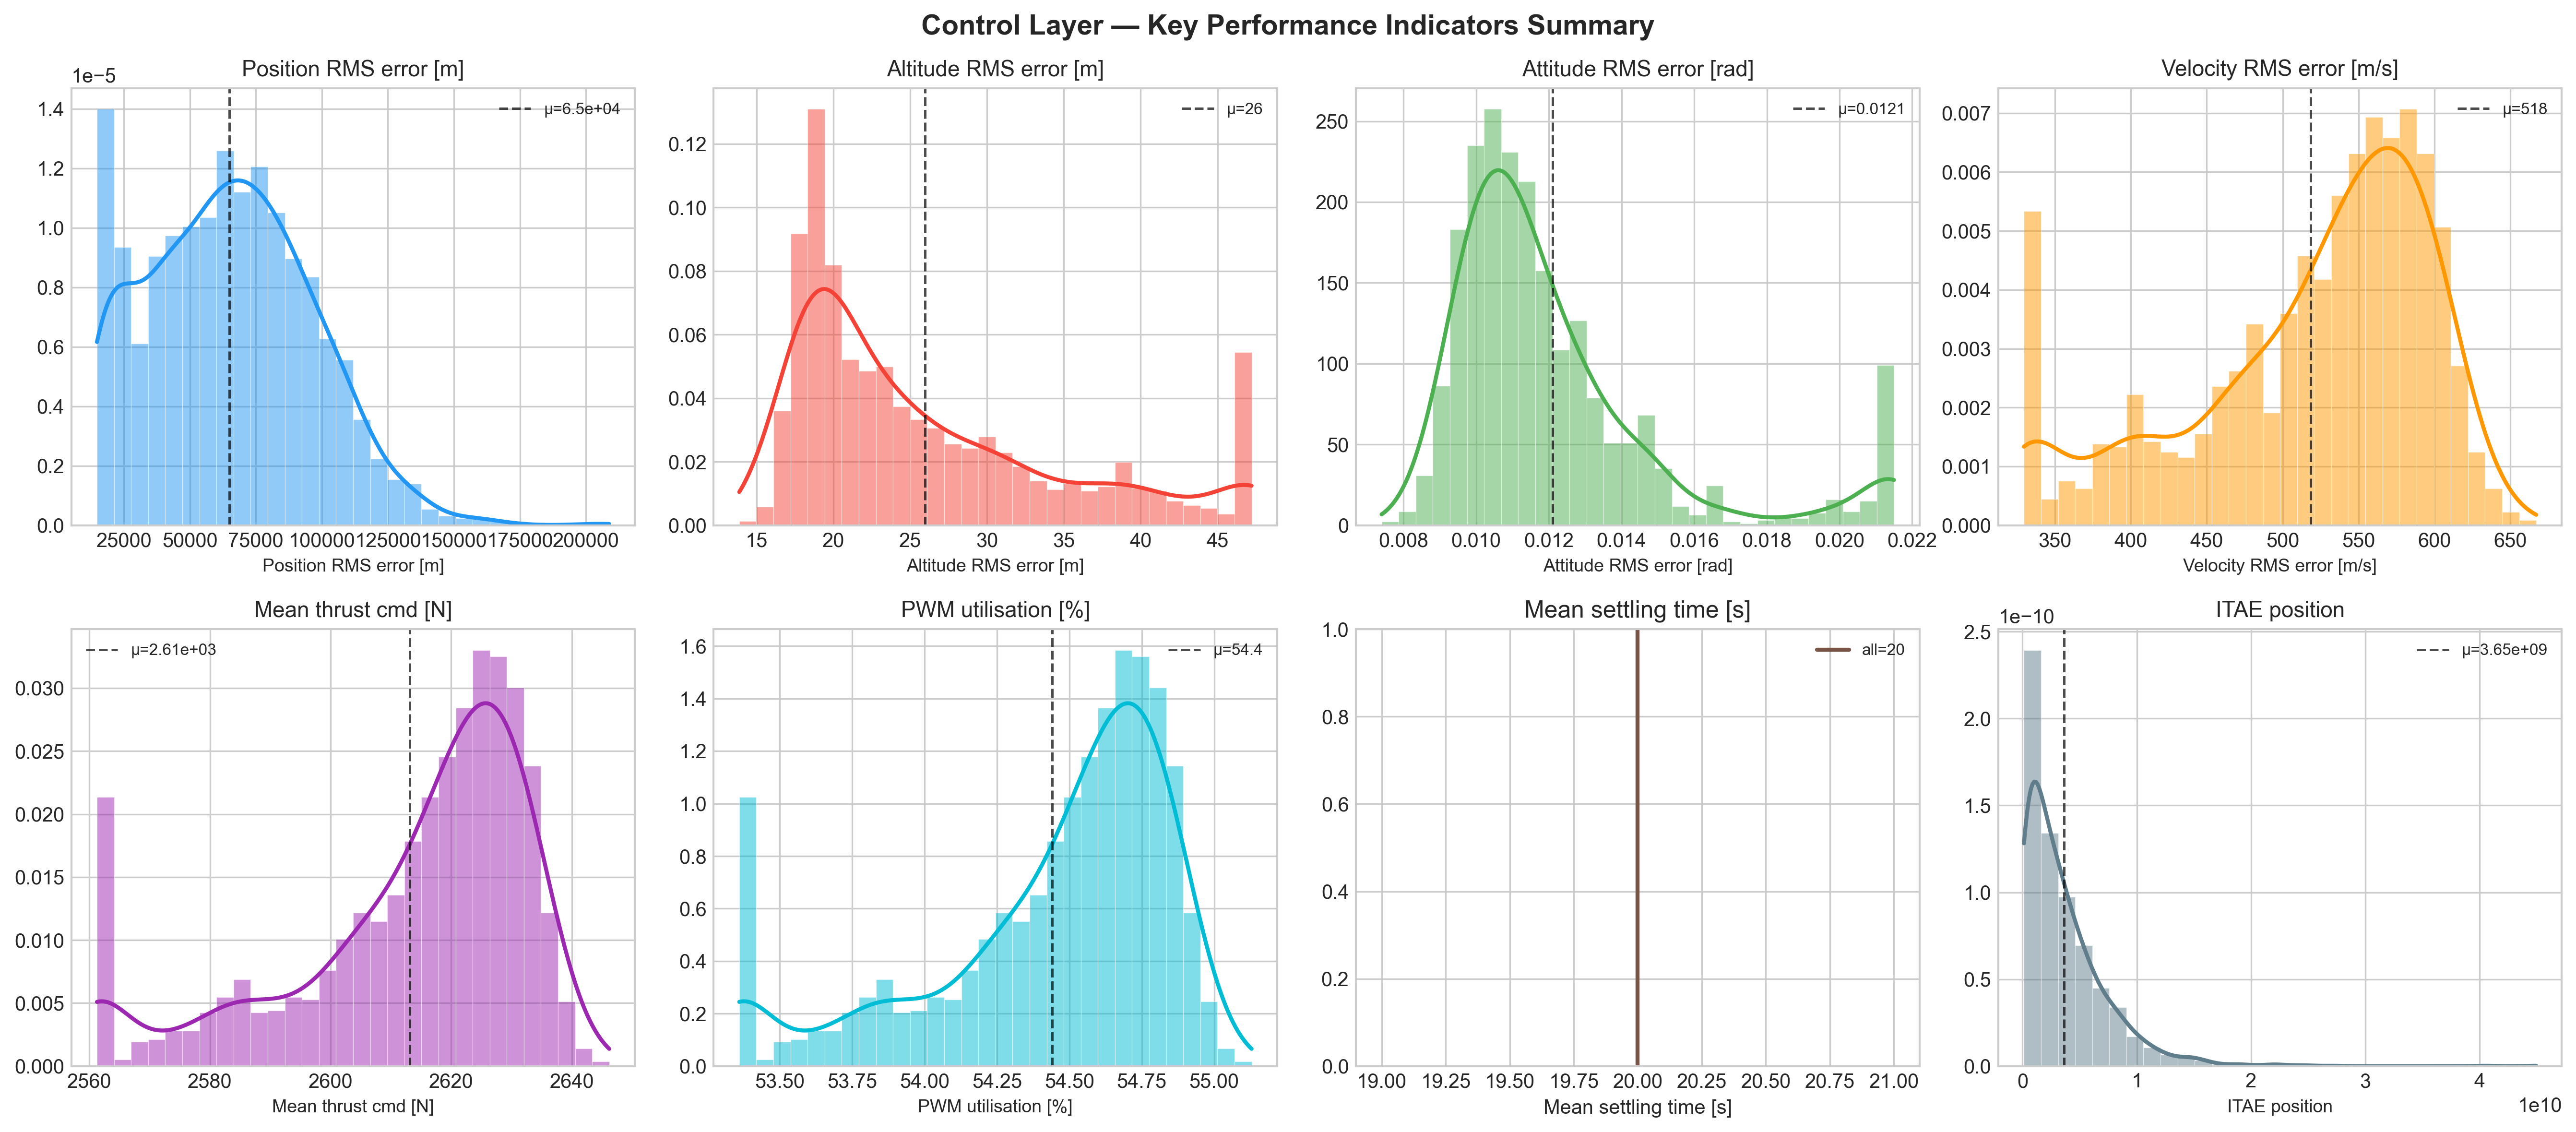
\includegraphics[width=0.72\textwidth]{figures/control_Z01_control_kpi_summary.png}
  \caption{Control KPI summary dashboard across all six original regions.
    Position RMSE, altitude RMSE, and ITAE scores are shown; mountain regions
    (Ladakh, Arunachal) exhibit higher variance due to wind disturbance
    at high altitude.}
  \label{fig:control_kpi}
\end{figure}

\end{document}
